%Implentation of a Total Power Radiometer in Software Defined Radios
%Thesis by Matthew E. Nelson
%In part for fullfillment of Masters of Science in Computer Engineering

% ISUTemplate file for a standard thesis
\documentclass[11pt]{isuthesis}
\usepackage[pdftex]{graphicx}
% Standard, old-style thesis
\usepackage{isutraditional}   \chaptertitle
% Old-style, thesis numbering down to subsubsection
\alternate
%package Tikz for doing diagrams
\usepackage{tikz}
\usetikzlibrary{arrows}
%Package listings for printing out Python and other code
\usepackage{listings}
\usepackage{rotating}
% Bibliography without numbers or labels
\usepackage{natbib}
\bibliographystyle{apa}
%\includeonly{titletoc,chapter1}
%Optional Package to add PDF bookmarks and hypertext links
\usepackage[pdftex,hypertexnames=false,linktocpage=true]{hyperref}
\hypersetup{colorlinks=true,linkcolor=blue,anchorcolor=blue,citecolor=blue,filecolor=blue,urlcolor=blue,bookmarksnumbered=true,pdfview=FitB}
\begin{document}
\DeclareGraphicsExtensions{.jpg,.pdf,.mps,.png}
% Template Titlepage File
\title{Re-configurable radiometer system using software defined radios}
\author{Matthew Erik Nelson}
\degree{MASTER OF SCIENCE}
\major{Computer Engineering (Embedded Systems)}
\level{master's}
\mprof{Phillip H Jones}
\members{John Basart \\ Mani Mina \\ Brian Hornbuckle}
\notice
\maketitle

% Optional thesis dedication
\chapter*{DEDICATION}

I would like to dedicate this thesis to my wife Jennifer who has stood by me through this long journey towards my Masters.  She put up with my countless afternoons that I was gone working on my thesis and also helped edit my thesis.  

I would also like to thank my parents, family and friends without whose support and encouragement enabled me to complete this work.


% Table of Contents, List of Tables and List of Figures
\pdfbookmark[1]{TABLE OF CONTENTS}{table}
\tableofcontents
\addtocontents{toc}{\def\protect\@chapapp{}} \cleardoublepage \phantomsection
\addcontentsline{toc}{chapter}{LIST OF TABLES}
\listoftables
\cleardoublepage \phantomsection \addcontentsline{toc}{chapter}{LIST OF FIGURES}
\listoffigures
% Comment out the next line if NOT using chaptertitle
\addtocontents{toc}{\def\protect\@chapapp{CHAPTER\ }}
%Optional Acknowledgements
\cleardoublepage \phantomsection
\specialchapt{ACKNOWLEDGEMENTS}

I would like to take this opportunity to express my thanks to those
who helped me with various aspects of conducting research and the writing
of this thesis.
First and foremost, Dr. Phillip Jones for his guidance, patience and support throughout this research and the writing of this thesis.
I would also like to thank Dr. John Basart who patiently spent many hours with me going over both the fundamentals and details with radiometers.
I would like to thank Dr. Brian Hornbuckle for his continued support and for allowing me to utilize his radiometer, lab and students towards my research.  
Finally I would like to thank Dr. Mani Mina who not only was instrumental in my undergraduate career but continued his support into my graduate path as well.  If it was not for Dr. Mina hiring me as the Chief Engineer of the Spacecraft Systems and Operations Lab, I would not be here today.

%Optional thesis abstract
\cleardoublepage \phantomsection
\specialchapt{ABSTRACT}

A software defined radio is defined as a communication system where components of a communication system that are typically done in hardware are now done in software.  The result is a highly flexible communication system that can adapt to changes to the system based on requests by the user or due to conditions in the radio frequency channel.  Software Defined Radios (SDRs) have been used for a variety of applications, mostly in the area of communications.  However, they have not been widely applied to remote sensing applications such as a radiometer.  A SDR based radiometer offers a very flexible and robust system more so than a more traditional radiometer which has fixed hardware and usually little room for flexibility and adaptability based on the needs of the radiometer application or due to changes in the radiometers environment.  The price of SDRs have also been steadily dropping making implementing them into radiometers a more attractive option compared to using traditional RF hardware.  In this thesis we will look into the feasibility and theory of using an off the shelf SDR hardware platform for a radiometer application.  In addition, we will look into how we can use the GNURadio software to create a total power radiometer within software and how this software can be used to make easy changes to the functionality of the radiometer.  Finally we will look at the preliminary results obtained from laboratory tests of the SDR radiometer system.

\newpage
\pagenumbering{arabic}
% Chapter 1 of the Thesis Template File
\chapter{INTRODUCTION AND  BACKGROUND}

%This is the opening paragraph to my thesis which explains in general terms the concepts and hypothesis which will be used in my thesis.

%This section will cover the basic and general concepts of my thesis.  This will be a high level approach to the problem and to the proposed solution.  In addition, this section gives a general background to the project

%This chapter has 4 sub-sections.  1)  Introduction to SDRs, 2) Introduction to GNURadio and 3) Introduction to the current ISU radiometer and finally the 4th is the Related Works section

\section{Introduction}
The goal of this thesis is to explore the use of a software defined radio that can function as well as or better than current radiometers.  In addition, we aimed to develop a radiometer that is more flexible than most radiometers and still maintain the accuracy and stability of a traditional radiometers if not exceed these specifications.  A secondary goal was to use off the shelf components that are generally more accessible and often less expensive.  This allows radiometers to be more accessible to a wider scope of researchers in this field.  And finally a tertiary goal was to ensure that the system as a whole is easy to use.  This ties to our secondary goal of making radiometers more accessible to a wider range of researchers and research topics.

This thesis looks to explore the following questions: (1) Can we use an off the shelf SDR along with GNURadio to recreate a radiometer in software that is easy to use and cost effective?  (2) If so, what performance can we get from the system?  (3) What benefits do we gain (if any) from using a SDR from a more traditional radiometer? The results of this research and experimentation are the subject of this thesis.

\subsection{Motivation}
Remote sensing allows us to collect information about the world that is around us.  This information can give us valuable information such as vegetation health, soil moisture, ocean salinity, and astronomy.  Using radiometers for remote sensing is fairly new, starting around 1960[\cite{Ulaby}].  Using radiometers for remote sensing has several advantages as we are able to look beyond certain obstacles that would otherwise be blocked in other remote sensing methods such as photography.  Radiometers have been used in the past for primarily astronomy in scanning for celestial objects that may be hidden from visual telescopes.  More recently radiometers have now been focusing on Earth and helping scientists to better understand the water cycle on Earth by monitoring our ocean salinity and soil moisture.  

\subsection{Software Defined Radio Radiometer}

A Software defined radio consist of both hardware and software that allow it to perform the operations of a radio or communication channel.  A software defined radio used for radiometer applications is identical to a software defined radio used for, as an example, a 802.11b radio with one major difference.  Since we need to amplify the signal more than what most communication applications require; we do require more powerful or additional LNAs to boost this signal.  In addition, since the first LNA plays a major role in the overall system noise and this system noise does affect performance of the radiometer, the selection of this LNA is important.  However, all other components are the same components used in other applications.

A software defined radio radiometer behaves analogous to a more traditional radiometer and thus the application is the same as a traditional radiometer.  This includes applications such as radio astronomy that includes applications in Earth Science such as soil moisture and ocean salinity[\cite{Ruf}].  A software defined radio radiometer can also allow for new application development that can expand the remote sensing field.  Since we have moved the majority of the hardware to software this allows us to further shrink the size and weight of the radiometer.  This allows for other radiometer applications such as Unmanned Aerial Vehicles (UAVs) for scanning soil moisture and ocean salinity remotely[\cite{McIntyre}].  

We will now introduce the three major components that make up a software defined radio radiometer.  

%\textbf{N200 SDR}
\subsubsection{N200 Software Defined Radio} 
The key component for a software defined radio radiometer is the software defined radio or SDR that will do most of the work as a radiometer through software.  The equipment selected for researching into this topic was the Ettus Research Group N200 SDR.  The SDR selected utilizes daughter boards as the RF front end to the SDR and up to two daughter boards may be installed into a N200.  This is an important consideration as one of the requirements is to be able to look at both the V-Pol and the H-Pol signal coming from the antenna.  By having a dual receiver SDR it is possible to correlate the signal and other signal analysis can also be done.  Another important reason the N200 is selected was due to its ability to handle up to 50 MHz of bandwidth to the computer and up to 25 MHz of RF bandwidth per daughter-board plugged in to the SDR.  This means that it is possible to have two receive cards that can stream up to 25 MHz bandwidth each.  

The N200 utilizes a flexible architecture for a variety of RF interface systems based on the frequency range desired and if receive and/or transmission is needed.  These daughter boards directly receive the RF signal and then outputs the analog I and Q signals that are then sampled by the N200 A/D converter for reception or receives the I and Q values from the N200 D/A converter for transmission. 

{\begin{figure}[h!tb] 
\centering
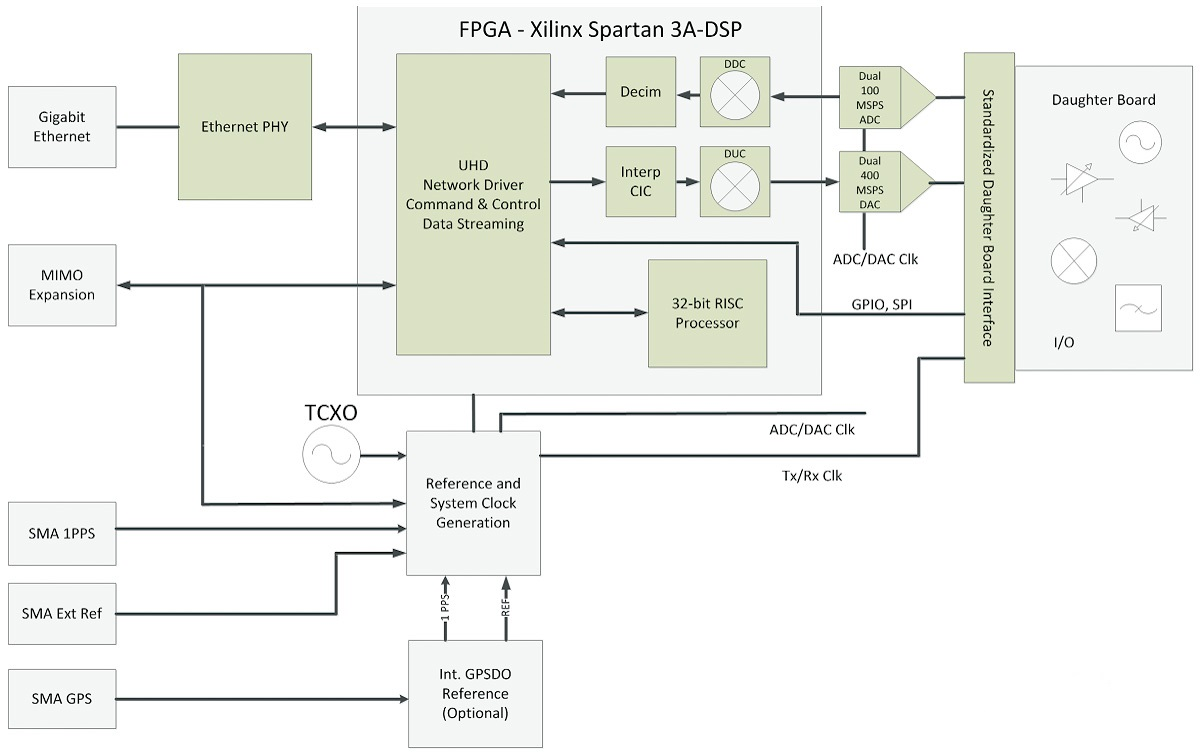
\includegraphics[width=14cm]{Images/n200_block_edited}
\isucaption{A block diagram of the Ettus N200 SDR}
\label{N200_block}
\end{figure}
}

The daughter board selected is the DBSRX2 card as this card is receive only and operates between 800 MHz and 2.4 GHz.  The DBSRX2 also has built in amplification that is adjustable through software.

\subsubsection{GNURadio Software}

For the software portion of the radio, we settled to use GNURadio, an open source software package that is well supported by the community and by the Ettus Research Group and the N200 SDR.  GNURadio also comes with what is known as GNURadio Companion or GRC.  This program provides us with a GUI interface and allows for the drag and drop of blocks that represent certain functions that can be used with the SDR.  GNURadio and GRC use Python as its main scripting language and GNURadio uses C++ code for directly accessing the hardware.  The hardware interface for the N200 is provided by Ettus through drivers that allow GNURadio to talk to the hardware.  Like GNURadio, these drivers are also available to all platforms.  Ettus has released these drivers to the open source community and continues to support the hardware drivers and GNURadio integration.

GNURadio operates on multiple platforms including Windows, Mac OS X, and Linux.  Linux is by far the most popular platform to work on and most of this thesis research was completed within the Linux environment.  Testing is also done though with a MacBook Pro running OS X 10.9.  The OS X implementation is well supported and is installed through MacPorts.  While windows is technically supported, it is often difficult to install and many of the libraries required are not 64-bit.  For these reasons windows was not used for executing GNURadio, but was used for some of the data analysis using Python.

Through GNURadio, we can now write code that will take the data given to us from the SDR and manipulate the signal as we need to mimic a radiometer.  The power detection, filtering and recording of this data is all done through GNURadio.  This also means that we are shifting more of the computational power done on the signal from the FPGA to a computer running GNURadio.  There are ways to change this behavior and upload code directly to the FPGA.  However, for this thesis it was easier to debug and work with GNURadio by keeping the processing on the desktop computer.  It does however mean that the host computer must be powerful enough to handle the signal and specifically the large bandwidth that we wish to send to it.  

\subsection{RF Front End}
The RF front end plays a critical role in the radiometer as the LNAs used in the front end has a large impact on the system noise generated by the radiometer itself.  A traditional radiometer utilizes both amplification through the LNAs and also includes filtering to the desired bandwidth.  A SDR radiometer does not require the filters as we are able to create these in software, however the amplification stages need to remain.  

{\begin{figure}[h!tb] 
\centering
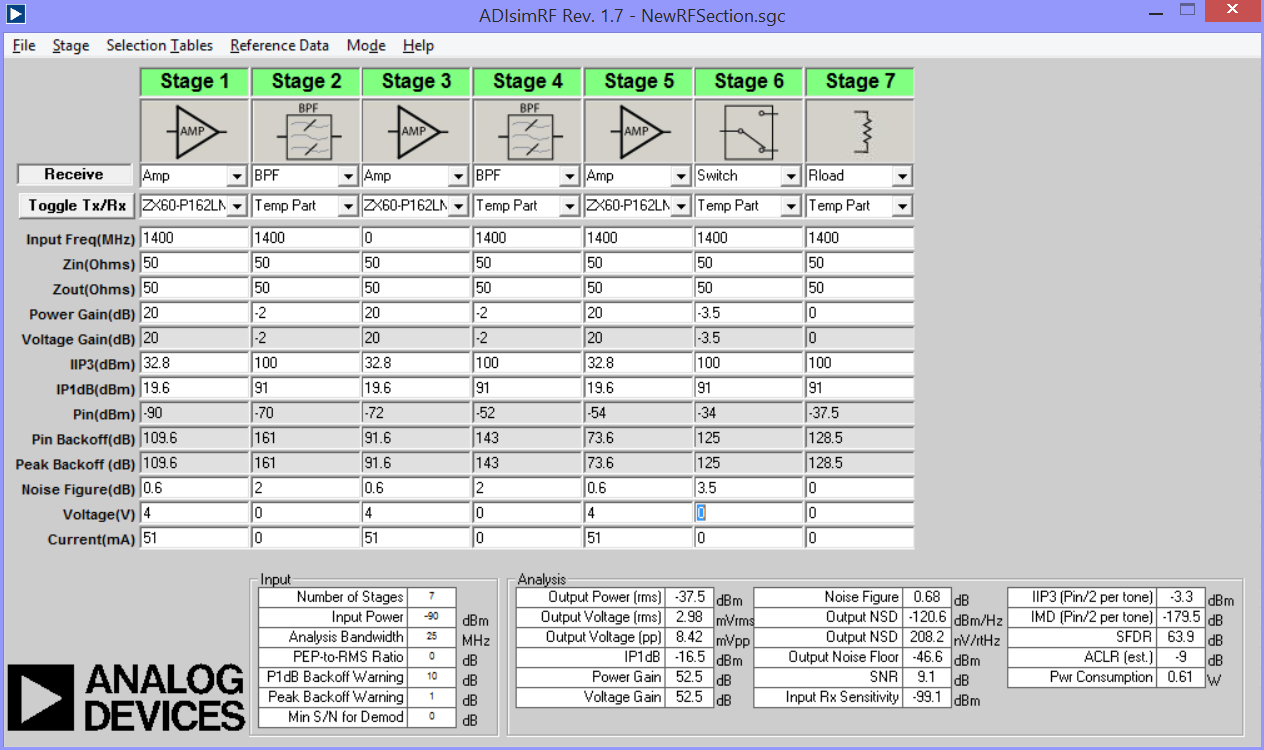
\includegraphics[width=0.8\linewidth]{Images/RF_Front_end.png}
\isucaption{The ADISIMRF program used to verify the design of the RF Front End}
\label{ISU_Rad}
\end{figure}
}
A typical RF front end uses a 3 stage Low Noise Amplifier (LNA) to amplifier the noise while keeping the noise contributed to the system as low as possible.  As with any radiometer, the first LNA is the most critical as it contributes the most to the overall system noise temperature.  For this reason a LNA that did not have a large gain but had a low noise figure is chosen. The second and third LNA has higher gain values at the cost of a higher noise figure, although not by much.  However, since they are further down the chain, they do not contribute as much to the total system noise.  The reason for this is further explained in chapter 3. 

\section{Background}
\textbf{Software Defined Radios} 
Software Defined Radios (SDRs) are used for a variety of applications but their primary application has been in the area of communications.  They appeal to applications where being able to change a modulation scheme or filter on the fly is desirable.  In these areas, SDRs often outperform a traditional hardware only radio with their ability to rapidly change their operations by simply changing their software.  Early SDRs were expensive due to the high costs in the analog to digital converters (ADCs) needed and in the high speed Field Programmable Gate Arrays (FPGA) used.  In recent years however, the cost of SDRs have decreased due to the cost of these key components decreasing in cost as well.  Even though the cost has gone down the performance of SDRs have increased and this has lead to new developments in applications for using SDRs in new and different ways.

The basic concept behind a SDR is that it will digitize the RF signal as soon as possible.  Once digitized, it is now evaluated by a computer, FPGA, or a dedicated System on Chip (SoC).  A canonical software defined radio architecture is one that consists of a power supply, antenna, multi-band RF converter, and a single chip that contains the needed processing and memory to carry out the radio functions in software [\cite{Mitola1995}]. This allows us to extract certain hardware functions, such as filtering, into the digital domain which can then be manipulated by software.  Since software is now manipulating the signal, we can rapidly change what functions we execute on the signal by changing the software.  This gives SDRs a high amount of flexibility as components that are normally done in hardware can now be done in software and can be changed by simply uploading new software or firmware to the system.  This also gives us a benefit in cost as certain components are no longer needed and changes done in software do not require additional hardware to be added or to be swapped out.

\textbf{Radiometers}  
Radiometers are radio receivers that simply listen to and record the amount of power received.  However, the power received is not a coherent signal, instead it is the amount of noise the radiometer sees.  Radiometers, at the basic level, listen to noise that is generated naturally from a source.  These sources can vary and the applications vary as well.  Some examples of radiometer applications have been in evaluating soil moisture content, ocean salinity levels, and celestial objects[\cite{ulaby2014}].

The amount of noise that is generated is due to the thermal agitation of the charge carriers, usually the electrons, which is directly correlated to the physical temperature of the source[\cite{Nyquist1928thermal}].  This correlation is done as a noise temperature.  All objects emit this noise and the intensity will vary on multiple parameters and on what the source is.  One source that has current research at Iowa State University is in detecting soil moisture.  Numerous soil types can be observed including sandy types of soil[\cite{Liu}], The brighter or warmer the noise temperature is, the more RF noise that has been received which correlates to a drier soil.  The less RF noise power received the cooler the noise temperature and this indicates wetter soil area. Radiometers such as these are already in service on satellites such as the Soil Moisture and Ocean Salinity (SMOS) satellite launched by the European Space Agency (ESA) and are used by scientists to monitor the Earth's soil moisture and ocean salinity[[\cite{McMullan}][\cite{Hardy}].  

A traditional radiometer uses multiple Low Noise Amplifiers (LNAs) to amplify the signal and filters to limit the bandwidth to a certain range.  Power is often measured using a square law detector and this is often an analog voltage output.  Even though we are measuring noise we want to measure the right noise and we want the noise generated by the radiometer hardware itself to be as low as possible.  In other words we are only interested in listening to the noise being generated from an outside source.  Additional noise in the system is impossible to eliminate, however we can take steps to reduce it as much as possible.  In addition, we can calculate what this noise is and take steps to account for it in our measurements.  However, this means that stability is another parameter within the radiometer.  If the noise generated within the radiometer is constantly changing then this makes it difficult to account for this additional noise.  There are steps we can take to work with this though.  A traditional method often used is the Dicke radiometer which switches between the measurement of the antenna and a known source[\cite{Dicke}].  By referencing this known source the Dicke radiometer can calibrate and account for any drift due to variations in the system.  Another method is to use highly stable components and keep them stable during the operation of the radiometer.  For LNAs, temperature directly effects the overall gain from the LNA.  In some radiometer applications we can control the temperature which allows us to keep the LNAs stable during the operation.  Stability will be discussed in greater detail later in this thesis.

Additional improvements to radiometers have also been done by digitizing parts of the radiometer.  The most common method for doing this is by digitizing the analog output of the square-law detector and sending that to a computer or processing unit to analyze the data[\cite{Bremer}].  While this does allow for easier computation and storage of the information it does not alleviate the needs to maintain stability or reduce possible additional noise of the system since this data is digitized after the RF signal chain.

\textbf{A more modern Radiometer}  
Iowa State University owns a 1.4 GHz, dual polarization, correlating radiometer.  This radiometer is in use by Dr. Brian Hornbuckle and his research team.  However, in recent years the radiometers digital circuitry has suffered from numerous issues which has made it unusable.  Part of the driving force behind this research in this thesis is to determine new methods that can be used to rebuild this radiometer.

The ISU Radiometer was built at the University of Michigan and put into service at ISU in 2006.  The ISU radiometer is unique in that it is one of the few direct sampling radiometers in use\cite{Erbas}.  This radiometer takes the RF signal, amplifies and filters the signal, and then sends it directly to an analog to digital converter.  At the time the ISU radiometer was built an A/D that is able to sample accurately at 1.4 GHz was expensive and hard to come.  However, the ISU radiometer does not sample at 2.8 GHz or above, instead it samples at 1.4 GHz.  The ISU radiometer is able to do this because it is only interested in power information.  This means that we are not interested in recreating the entire signal and therefore we can under-sample the signal.  The A/D data is then sent to a Field Programmable Gate Array (FPGA) which then processes the data.  The ISU radiometer is also a correlating radiometer which means that it looks at both the vertical polarization (V-Pol) and the horizontal polarization (H-Pol) and then correlates this information[\cite{Fischman2001}].  

\section{Related Works}
As mentioned before, software defined radios have been used in a number of applications.  While as far as the author has determined, this is the first application of using an off the shelf software defined radio for a radiometer in remote sensing for soil moisture measurements, there has been similar applications done.  The closest application that has been found is with radio astronomy.  Radiometers used in radio astronomy is nothing new and has been used for some time now[\cite{Ohm}]. There are similarities between radio astronomy and remote sensing of the ground.  Both are using a radiometer to listen to a source of interest.  With radio astronomy the basic principle is that a hot source such as a star will produce more noise than the cooler background of space.  In remote sensing we are looking at the overall change of the source to determine its characteristics.  Both cases are measuring the total power of the noise and based on that information we can determine some properties of the source we are looking at.

\subsection{Radio Astronomy Examples}
The Shirleys Bay Radio Astronomy Consortium (SBRAC) located in Smiths Falls, Ontario is using the USRP software defined radio in conjunction with GNURadio.  SBRAC has successfully used this configuration to obtain radio astronomy data by looking at the hydrogen line at 1420.4058 MHz [\cite{Leech2007}].  The person in charge of this facility, Marcus Leech, contributed software to the GNURadio specifically for radio astronomy applications.  It was this software branch that was used as the base for the GNURadio program that was used in this thesis.  Marcus Leech continue to contribute to the GNURadio community and continues to provide support for these functions as well[\cite{Leech}].

Another example of a software defined radio used as a radiometer is from students at the University of Illinois and Grand Valley State University that built a software defined radio to listen to emissions from Jupiter[\cite{Behnke}].  This software defined radio was built using an Analog Devices AD9460 and a Xilinx Spartan-3E-500 FPGA to build the SDR itself.  A RF front end was also built to filter and amplify the signal coming into the SDR.  Finally, this group also used GNURadio to interface to and talk to the SDR and used both Python and wxGUI to build a working interface.  The students reported that the SDR radiometer worked well and was able to do so at a low price point.

It should be noted that much of the related works found worked with using a radiometer for astronomy or for looking at the sky.  For the ISU radiometer however we are looking at the ground and we are using the radiometer for soil moisture instead of measuring stars and other points of interest in the sky.  While the fundamentals is the same for either radiometer some adjustments need to be made because a radiometer that is looking at the sky often sees a cool brightness temperature whereas a radiometer looking at the ground sees a much warmer brightness temperature.  This is due to the albedo of the Earth having a much warmer noise temperature then what you find with radio astronomy[\cite{Tiuri}].
\subsection{Other Digital Radiometers}

A digital radiometer is not a new concept.  Early radiometers often digitize the analog voltage information from the square-law detector and then send that information to a computer for storage or analysis.  

A pre-cursor to a software defined radio, some radiometers also digitize the incoming RF signal, but under-sample this information.  Since only power is the only information desired for these radiometers, this was acceptable.  However, these radiometers did often use the same components you might find in a software defined radio such as an A/D converter and FPGA.  These components however were used in different ways.

One reason why these devices were used differently from a SDR was due to cost.  Most radiometer operations happen at 1.4 GHz or above.  A/D converters at these higher frequencies become more expensive and harder to obtain.  In recent years however, these costs have come down.

The major difference between other digital radiometers and what is discussed in this thesis is that we retain both phase and magnitude information and instead mimics a traditional radiometer in software by summing and squaring the I and Q values and then running this information through a low-pass IIR filter.  By retaining this information, we can perform a more in-dept analysis of the signal coming into the radiometer which allows for greater agility in the system.

\subsection{RFI Mitigation}
Radio Frequency Interference (RFI) is a common problem with a nearly all radiometers.  This problem is often exasperated with satellite radiometers since those radiometers see a large area on the ground.  Previous missions such as the Soil Moisture Ocean Salinity (SMOS) satellite has numerous issues with RFI that skews the data that they collect.  There have been a number of methods to either work around the RFI or attempt to filter it using mechanical filters.  University of Michigan has done a number of experiments in detection and mitigation of RFI with the use of mechanical filters [\cite{DeRooRFI}].  And a number of papers have been published on the detection of RFI in radiometers [\citep{DeRoo}][\cite{Forte}].

In all of these cases the radiometers used do not retain frequency information and thus must use other methods to detect and try to mitigate the signal.  In this thesis we cover a way to mitigate RFI and are able to do so using software to define a filter to notch out the offending signal.  Detection in a software defined radio radiometer is easier as we have both power and frequency information to design the filter.
% Chapter 2 of the Thesis Template File
%   which includes bibliographic references.

%Chapter 2: Related Work  
%1) Introduction paragraph summarizing the flow/content/structure of the Related Work, while describing how the areas of related work are logically connect to your work  
%2) Related area 1 
%3) Related area 2  
%4) Related area 3
%5) Within each related area, point out in what why your work is different from the existing work.

\chapter{RELATED WORKS}\label{ch:relatedworks}

Three areas closely related to the work in this thesis are: digital radiometers, software defined radio based radiometers, and radio frequency interference (RFI) mitigation.  This chapter first presents two classifications of digital radiometers (hybrid and direct sampling).  Next, software defined radio based radiometers are discussed in their own section, as a third classification of digital radiometer.  This chapter concludes with a brief overview of the topic of RFI, which is important to consider when deploying radiometers.

\section{Digital Radiometers}

A digital radiometer replaces portions of a traditional radiometer's analog components with digital components[\cite{Ruf}].  Two types of digital radiometers include: hybrid and direct sampling.

\emph{Hybrid.}  A hybrid radiometer uses a mixture of  analog and digital components[\cite{skou}].  Often the analog voltage output from the diode of a square law detector, which is used to indicate the total power observed, will be digitized. 

\emph{Direct Sampling.}  A direct sampling radiometer can be considered a type of hybrid radiometer that directly samples the incoming RF signal and then uses digital signal processing techniques to extract total power information.  As an example, Iowa State University (ISU) owns a 1.4 GHz, dual polarization, correlating radiometer that uses direct sampling.  It was built by the University of Michigan and put into service at ISU in 2006 [\cite{Erbas}].  This radiometer takes the RF signal and using analog components amplifies and filters the signal, and then sends it to an analog to digital converter.  The radiometer is designed to operate in the protected spectrum of 1400 MHz to 1420 MHz.  Unlike other radiometers discussed, this radiometer samples the incoming RF signal at 1400 MHz.  This method allows for power information to be extracted, however the full signal can not be recreated due to Nyquist's theorem [\cite{Fischman2001}].

Both hybrid and direct sampling radiometers are designed to retain only the total power information contained in a RF signal.  While measuring total RF power is the primary purpose of a radiometer, as it will be discussed later, retaining phase and frequency information can be useful as well.

\section{Software Defined Radio Based Radiometers}

Software defined radio based radiometers can be considered a relatively new subclass of digital radiometer.  With the advent of software defined radios that are wildly available, there has been increasing interest in applying this technology to radiometers.  This section discusses two works that have explored using software defined radio technology in radiometry from the Shirley's Bay Radio Astronomy Consortium and from Grand Valley State University.

\emph{Shirleys Bay Radio Astronomy Consortium.}  The Shirleys Bay Radio Astronomy Consortium (SBRAC) made use of a software defined radio to restore a radio telescope used for radio astronomy.  They attached a software defined radio to their eighteen meter radius dish to obtain astronomical information by observing the hydrogen line located at 1420.4058 MHz in the RF spectrum[\cite{Leech2007}].  Marcus Leech, who headed SBRAC, contributed software to GNURadio specifically to support radio astronomy applications.  This branch of GNURadio was used as the software base used in this thesis [\cite{Leech}].

While parts of the GNURadio software used in this thesis were derived from Marcus Leech's work, additional features were added such as offending signal detection, offending signal mitigation, and a software implemented noise generator.  Additionally, elements of the graphical user interface (GUI) were enhanced to aid in data visualization and analysis data.  For example, a waterfall display of a signal spectrum over time was implemented.

\emph{Grand Valley State University.}  In 2013, the University of Illinois and Grand Valley State University built a software defined radio based radiometer to listen to emissions from Jupiter[\cite{Behnke}].  They custom built the hardware portion of their software defined radio using an Analog Devices analog to digital converter (AD9460) and a Xilinx (Spartan-3E-500) FPGA.  They also implemented a RF front end to filter and amplify the incoming RF signal.  The software side of their radiometer was composed of: 1) GNURadio for low-level communications with their software defined radio and, 2) Python script and WxGUI to implement a higher level user interface.  The students reported that their SDR based radiometer worked well at a low price point.  One aspect that differentiates the work in the thesis from Grand Valley State University's work is that they build their own custom hardware for their software defined radio, while in this work off the shelf components where used with an aim of making radiometers more wildly accessible to the research community.

\section{Radio Frequency Interference (RFI) Mitigation}
When an RF signal generated by a source other than the object (or phenomena) of interest interferes (i.e. masks or contaminates) with the RF signal of interest this is referred to as radio frequency interference (RFI).  Radio Frequency Interference (RFI) is a common problem with nearly all radiometers because they are highly sensitive receivers, thus even small unwanted signals can have a large negative impact on a radiometer based experiment.  It is for this reason certain frequency bands have been designated as protected frequencies' for radiometer use, by the international community.  However, not all entities abide by these standards.  For example, the satellite radiometer used by the Soil Moisture Ocean Salinity (SMOS) mission has had numerous issues with RFI [\cite{Kerr}] skewing their data and in some cases making the data unusable for soil moisture measurements [\cite{Richaume}].  

The area of RFI detection and mitigation is still an active field of research [\cite{Forte}].  With respect to RFI detection, since radiometers typically do not retain spectral frequency information, statiscal methods have been explored that loot at variations in the received power to determine when RFI is occurring.

One such method is the kurtosis statistic method[\cite{DeRoo}] (or polarization signature) method.  With respect to RFI mitigation, mechanical filters are used to selectively filter out the offending signals [\cite{DeRooRFI}].  

While mechanical filters are an effective means of RFI mitigation, they add both weight and complexity to the radiometer.  For example, multiple filters would be required to isolate and remove frequency bands that contain the offending signal(s).  One idea this thesis explores is making use of frequency information and software-based digital filters for RFI detection and mitigation.


%----------------------------------------------------------
% End of Chapter 2.  Anything below this is extra information


% Chapter 3 from the thesis template file
%   that contains an example table and figure.

%Chapter 3: Background
%1) Introduction paragraph summarizing the flow/content/structure of the Background chapter
%2) Radiometer Basics
%	a) Power Detection
%	b) Integration and filtering
%	c) Metrics
%		i) Sensitivity
%		ii) Stability
%	d) Implementation
%3) Software Defined Radio Basics
%	a) High-level figure of the components of a generic SDR.
%	b) SDR Operation
%	c) GNURadio Operation
%4) Software Defined Radio Development Platform (i.e. your specific platform)
%	a) Hardware (i.e. N200)
%	b) Software (i.e. GNU Radio)  

\chapter{BACKGROUND}\label{ch:background}

This chapter will examine background information on the basic operation of a radiometer, a software defined radio and background on the development platform used to build a software defined radiometer.  We begin with an overview of a traditional radiometer and how this type of radiometer works.  This is followed by high level examination on how a software defined radio operates.  Finally we will discuss both the hardware and software selected and used for our development platform to create this software defined radiometer.

\section{Radiometer Basics}\label{rad_basics}

The primary task of a radiometer is to measure power, or more precisely, to accurately measure the correct power within a certain degree of accuracy.  In order to accurately and within a high degree of precision measure power a radiometer must take into account factors such as the system noise, the bandwidth of the signal and the stability of the system as a whole[\cite{Evans}]. 

The amount of noise that is generated by the object of interest is due to the thermal agitation of the charge carriers, usually the electrons, which is directly correlated to the physical temperature of the source [\cite{Nyquist1928thermal}].  It is because of this correlation that we often refer to the amount of noise received as the noise temperature and it is measured in Kelvins. 

%The amount of noise that is generated by the object of interest is due to the thermal agitation of the charge carriers, usually the electrons, which is directly correlated to the physical temperature of the source[\cite{Nyquist1928thermal}].  This correlation is done as a noise temperature.  All objects emit this noise and the intensity will vary on multiple parameters and on what the source is.  One source that has current research at Iowa State University is in detecting soil moisture.  Numerous soil types can be observed including sandy types of soil[\cite{Liu}], The brighter or warmer the noise temperature is, the more RF noise that has been received which correlates to a drier soil.  The less RF noise power received the cooler the noise temperature and this indicates wetter soil area. Radiometers such as these are already in service on satellites such as the Soil Moisture and Ocean Salinity (SMOS) satellite launched by the European Space Agency (ESA) and are used by scientists to monitor the Earth's soil moisture and ocean salinity[[\cite{McMullan}][\cite{Hardy}].  

In all radiometers there are six stages that is common in all radiometers.  They are:

\begin{enumerate}
\item Source (antenna or $T_{A}$)
\item Amplification (Gain or $G$),
\item Bandwidth ($\beta$),
\item Power detection ($X^{2}$),
\item Integration ($\tau$),
\item Output (Voltage, rQ or Kelvin).
\end{enumerate}

Figure \ref{trad_radiometer} shows each stage as they relate to each other.  We begin with our source which is often an antenna.  Amplification or gain in the system then amplifies this signal so that it is easier to measure changes in our noise.  Our bandwidth is often restricted by filtering and can occur before or after the amplification stage and in some cases filtering is done before and after the filtering stage.  Power detection extracts the power information from the signal.  Because the signal is often noisy, we use integration to smooth our signal and improve our sensitivity.  Finally our output is the total power information.  This information may be as simple as a voltage output, an uncalibrated value referred to as rQ, or may be a calibrated noise temperature measured in Kelvins.

{\begin{figure}[h!tb] 
\centering
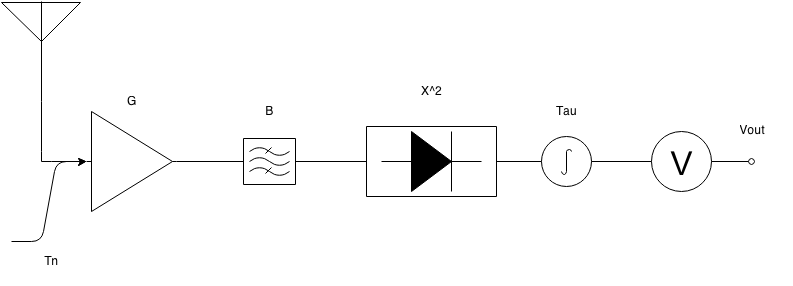
\includegraphics[width=\textwidth]{Images/Radiometer.png}
\isucaption{A total power radiometer block diagram}
\label{trad_radiometer}
\end{figure}
}

In figure \ref{trad_radiometer} we have one more component that is common in all radiometers but is not a physical component or stage in the radiometer.  That item is additional noise that gets added to the system from within the system itself is called system noise or $T_{N}$.

In addition to the system noise, another very common problem with radiometers is stability.  Most instabilities in a radiometer are due to fluctuations that occur in the amplification stage or the Low Noise Amplifiers (LNAs) used. There are two factors that cause changes in the gain values, voltage feeding the LNA and the physical temperature of the LNA.  These gain fluctuations can be controlled to a point by closely monitoring and controlling both the voltage and the temperature of the LNAs. However, this is not an easy task and in some cases is not practical.  Therefore, other methods have been developed to compensate for these fluctuations.  There are three common types of radiometers designed to adjust for gain fluctuations.  They are:

\begin{enumerate}
\item Dicke radiometer,
\item Noise injection radiometer,
\item Polarimetric or correlating radiometer.
\end{enumerate}

%Additional noise in the system is impossible to eliminate, however we can take steps to reduce it as much as possible.  In addition, we can calculate what this noise is and take steps to account for it in our measurements.  However, this means that stability is another parameter within the radiometer.  If the noise generated within the radiometer is constantly changing then this makes it difficult to account for this additional noise.  

One of the first methods used is the Dicke radiometer which switches between the measurement of the antenna and a known noise source[\cite{Dicke}].  By referencing this known source very quickly the Dicke radiometer can account for and greatly reduce gain fluctuations.  

{\begin{figure}[h!tb] 
\centering
\includegraphics[width=\textwidth]{Images/Dicke_block.png}
\isucaption{A block diagram of a Dicke radiometer}
\label{dicke_radiometer}
\end{figure}
}

While a Dicke radiometer greatly reduces the fluctuation in the gain of the radiometer and improves stability, it does so at the cost of not seeing the object of interest while it is referencing the known source.  This decreases the overall sensitivity of the radiometer.

{\begin{figure}[h!tb] 
\centering
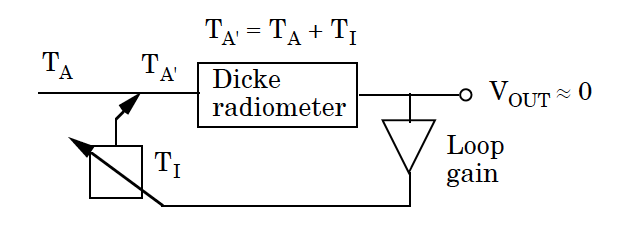
\includegraphics[width=\textwidth]{Images/NoiseInj_block.png}
\isucaption{A block diagram of a Noise Injection radiometer}
\label{NoiseInj_radiometer}
\end{figure}
}

A noise injection radiometer is a variation of the Dicke radiometer where a variable noise source is used and injected into the RF chain as seen in Figure \ref{NoiseInj_radiometer}.  The output of this noise source is then adjusted so that the noise input plus the signal from our source is equal to the reference noise.  This completely eliminates the gain fluctuations however increases the system noise which also reduces our sensitivity of the radiometer.

Our source signal is often times assumed to be not polarized.  However, this is not the case and an incoming signal often has some polarization.  A correlating radiometer [\cite{Fujimoto}] uses a dual polarization antenna to split the vertical and horizontal polarization of the signal.  Each of these signals is then fed into a radiometer and is correlated.  Since gain fluctuations or uncorrelated, they are reduced in the system.  This reduces gain fluctuations and also helps maintain the sensitivity of the radiometer.  However it adds a much greater complexity to the radiometer and requires two identical receivers.  

%Additional improvements to radiometers have also been done by digitizing parts of the radiometer.  The most common method for doing this is by digitizing the analog output of the square-law detector and sending that to a computer or processing unit to analyze the data[\cite{Bremer}].  While this does allow for easier computation and storage of the information it does not alleviate the needs to maintain stability or reduce possible additional noise of the system since this data is digitized after the RF signal chain.

\subsection{Measuring RF power}

To measure power in a radiometer, several factors are taken into consideration.  To begin with we have the noise signal coming from the antenna.  Our antenna is assumed to be looking at our target of interest and it is assumed that we can relate the antenna noise to the noise from the source.  It is often easier to refer to this noise as the brightness temperature.  Therefore, the brightness temperature of the source can be related to the brightness temperature at the antenna.  We will refer to this brightness temperature as $T_{A}$.  

%{\begin{figure}[h!tb] 
%\centering
%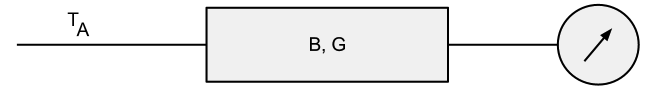
\includegraphics[width=\textwidth]{Images/simple_rad.png}
%\isucaption{The ideal radiometer block diagram}
%\label{simplerad}
%\end{figure}
%}

%Figure \ref{simplerad} shows us an ideal radiometer.  That is a radiometer that has an input from the antenna, $T_{A}$, a known bandwidth denoted as $B$ or $\beta$ and a known gain denoted as $G$.  At the end of the block is the detector, which measures the power from the radiometer.

%Only a certain selection of the radio spectrum is observed by the radiometer and this is the bandwidth of the radiometer.  In our scenario, we center around 1.4125 GHz.  There is a reason why 1.4125 GHz is selected and that is from 1.4000 to 1.4250 GHz is protected internationally to be as radio frequency interference free as possible.  This reduces interference from outside sources such as transmitters that can interfere with the operation of the radiometer.  

%The power coming from the antenna is the combination of the following items:

%\begin{enumerate}
%\item Gain or $G$ of the system,
%\item Bandwidth or $\beta$ of the system,
%\item Signal source or $T_{A}$.
%\end{enumerate}

To calculate our power from the radiometer, we multiply each item with the Boltzmann constant referred to as \textit{k}. Equation \ref{eq:power_rad_eq} gives us the total power, in watts, of an ideal radiometer.

\begin{equation} \label{eq:power_rad_eq}
P=k*\beta*G*(T_{A}) (watts)
\end{equation}

As discussed in section \ref{rad_basics}, the system noise is another component of the radiometer that needs to be addressed.  Figure~\ref{trad_radiometer} shows the additional noise that is injected into the system.

%{\begin{figure}[h!tb] 
%\centering
%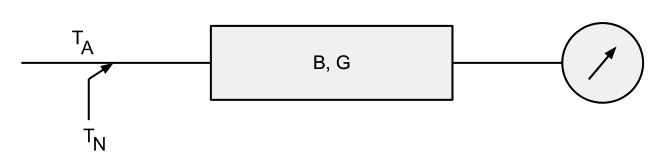
\includegraphics[width=\textwidth]{Images/radiometer_noise_added.png}
%\isucaption{A more realistic radiometer model}
%\label{noiserad}
%\end{figure}
%}

As it can be seen, this additional noise is added to the noise coming from the antenna source.  Therefore, T$_{N}$ is added to T$_{A}$ and our final equation for the power measured is shown in equation~\ref{eq:final_power}.  

\begin{equation} \label{eq:final_power}
P=k*\beta*G*(T_{A}+T_{N}) (watts)
\end{equation}

Figure \ref{trad_radiometer} showed us a more typical radiometer and was discussed in the previous section.  However, power detection and the associated voltage output has not been discussed.  Power detection is accomplished typically with a square-law detector and this output is often run through an integrator to smooth the output[\cite{Leinweber}].  Finally we have the output which is a voltage represented as V$_{out}$.  This results in equation~\ref{eq:vout_1}.

\begin{equation} \label{eq:vout_1}
V_{OUT}=c*(T_A+T_N)*G
\end{equation}

Here V$_{OUT}$ is shown by the addition of both the noise from the system T$_N$ and the noise from the antenna, T$_A$ and multiplied by the gain in the system, $G$ [\cite{skou}].  A constant factor $c$ is useful for when we are looking at a radiometer like a Dicke radiometer in which the value of $c$ is $\frac{1}{2}$.  In most applications outside of a Dicke radiometer, $c$ is 1 and can be ignored.  

The voltage output from this radiometer is then either measured or may also be sampled by an analog to digital converter.  This voltage then represents the total power measured by the radiometer, however this measurement is not calibrated.

%Most radiometers are more complicated than the one shown in Figure~\ref{noiserad}.  Additional signal conditioning is often needed which filters and may also amplify or attenuate the signal as required for proper performance through the RF chain.  Once the total power is detected a method to measure and store this reading must also be done.  Finally, additional hardware may be required to stabilize the radiometer which will be discussed in more detail in this thesis.

\subsection{Integration and filtering}

Filtering with a traditional radiometer is usually accomplished by using mechanical filters.  Often these are band-pass filters that limit the bandwidth that the radiometer sees.  Other filters, such as a low pass filter are also used, but usually to smooth out the output from the square law detector.  Another item used to help smooth out the signal from the square law detector is an integrator.

A RC filter is analogous to an integrator where the R and C values determine our time constant and our integration time for the filter[\cite{Aitken}].  We know a RC filter is analogous to an integrator by looking at equation \ref{eq:rc_int}.

\begin{equation}\label{eq:rc_int}
\frac{1}{RC}\int{V_idt}
\end{equation}

To begin with, we look at what an analog RC filter looks like. 

{\begin{figure}[h!tb] 
\centering
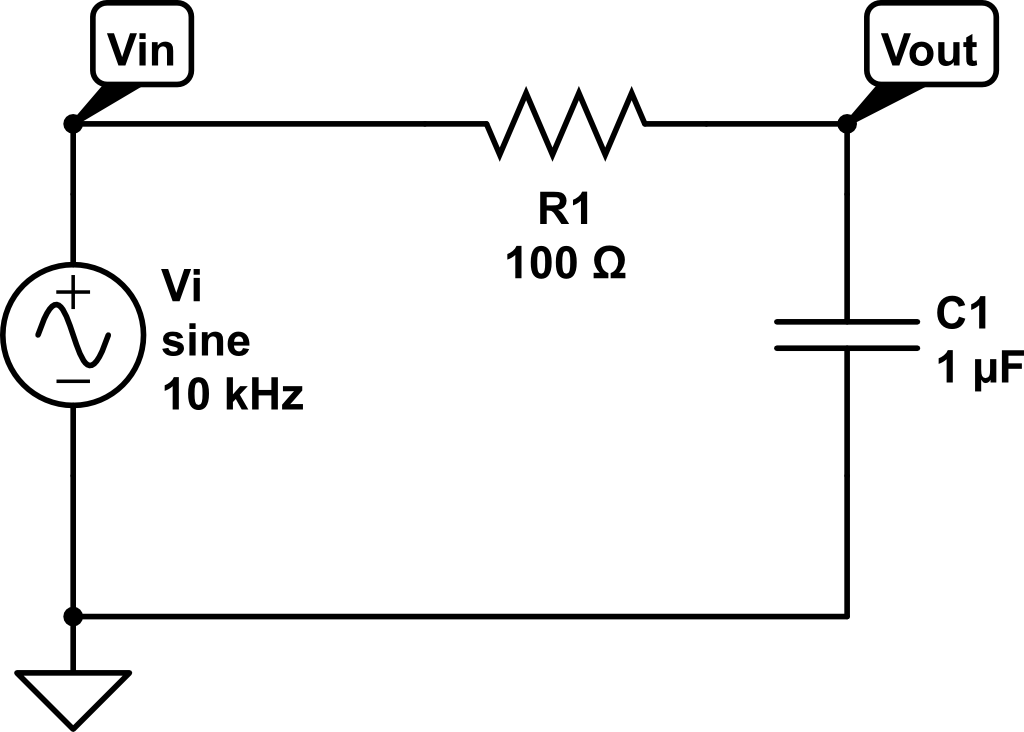
\includegraphics[width=10cm]{Images/rc-circuit.png}
\isucaption{A simple RC circuit}
\label{rc_circuit}
\end{figure}
}

This circuit can be represented by equation \ref{eq:rc_circuit_eq}.

\begin{equation}\label{eq:rc_circuit_eq}
\frac{V_{in}-V_{out}}{R}=C\frac{dV_{out}}{dt}
\end{equation}

This integration smooths out the signal from the square law detector and also improves our sensitivity of the radiometer.  This will be further explained the next section.

\subsection{Radiometer Performance Metrics}
There are two criteria that determines how well a radiometer performs.  The first criteria is with the sensitivity of the radiometer.  This tells us how well the radiometer can differentiate between the information we want and the noise we do not want.  The second criteria is stability.

\emph{Sensitivity}.  Sensitivity of the radiometer relates to the amount of power that the radio selects from the antenna.  This selection is then dependent on the bandwidth that the radiometer is able to listen to.  The radiometer however detects not only the signal of interest but also receives a noise signal as well.  This noise is added to the signal and can not be separated from the signal.  Because this noise is added to the signal, we must be able to determine a change in the signal while the noise signal is also present.  

To understand this, let us look at the example of T$_{A}$ has a value of 200 K and T$_{N}$ has a value of 800 K.  Since T$_{N}$ is added to our antenna signal, we have a total noise temperature of 1,000 K.  This means that if we want to detect a change as small as 1 K, we must be able to measure the difference between 1,000 K and 1,001 K[\cite{skou}].

%Equation \ref{eq:final_power} shows us the total power from the radiometer, where we take into consideration bandwidth, gain and the input from the antenna plus the noise added from the antenna.  

The ability of a radiometer to detect these small changes is the radiometer's sensitivity, or the standard deviation of the output signal from the radiometer.  This sensitivity is also referred to as the Noise Equivalent Delta ($\Delta$) Temperature or NE$\Delta$T and is shown in equation \ref{NEAT_EQ}. 

\begin{equation} \label{NEAT_EQ}
NE\Delta T=\frac{T_{A}+T_{N}}{\sqrt{\beta * \tau}} 
\end{equation}

The sensitivity of the radiometer is based on both the bandwidth, $\beta$, of the incoming signal and the integration time, $\tau$.  As it can be seen in equation \ref{NEAT_EQ}, we want to have as much bandwidth as possible.  In a traditional radiometer, this bandwidth is often fixed and is dependent on the band-pass filters used in the radiometer.  We can however control $\tau$ and a longer integration time will help improve the sensitivity of the radiometer to a certain degree.[\cite{ulaby}]

\emph{Stability.}  Stability and accuracy are additional problems that need to be considered when looking at the radiometer system.  To begin we can once again look at the power received equation \ref{eq:final_power}.

As we look at this equation, we can see that if $k$, $\beta$, $G$, and $T_{N}$ are constant, then stability can be assured.  The Boltzman constant $k$ is a known constant and we can also assume that our bandwidth, $\beta$, will also remain constant.  Gain and the noise temperature however will vary.  

Fluctuations in gain is the largest factor that affects stability in the system and this can be seen in equation \ref{eq:rad_stability}.  As discussed earlier, it is this factor that has been a driving force for changes to the design of a radiometer as demonstrated by the Dicke and Correlating radiometer designs.  

Gain fluctuations are caused by two factors: the physical temperature of the amplifier and the voltage that feeds the amplifier.  High accuracy voltage regulators can help control fluctuations in voltages that can in turn affect the gain.  A factor however that is harder to control is temperature.  Various methods have been used to control the temperature when the radiometer is used in fluctuating temperature environments such as the outdoors or in space.  

\begin{equation} \label{eq:rad_stability}
\Delta T_G=T_{sys} \left(\frac{\Delta G}{G}\right)
\end{equation}

With stability we need to either attempt to stabilize the radiometer as best as we can or compensate for the gain fluctuations.  Compensation has been discussed and three types of radiometers have been identified that attempt to compensate for these fluctuations.  To control the stability many radiometers will use highly accurate voltage regulators and will control the temperature of the LNA through methods such as thermal electric coolers.  Other methods to control or account for instability has lead to the development of other types of radiometers such as the ones discussed in section \ref{rad_basics}.

%\subsection{Implementation of traditional radiometer}
 
\section{Software Defined Radios Basics} 
The basic concept behind a SDR is that it will digitize the RF signal as soon as possible.  Once digitized, it is now evaluated by a computer, FPGA, or a dedicated System on Chip (SoC).  A canonical software defined radio architecture is one that consists of a power supply, antenna, multi-band RF converter, and a single chip that contains the needed processing and memory to carry out the radio functions in software [\cite{Mitola1995}]. This allows us to extract certain hardware functions, such as filtering, into the digital domain which can then be manipulated by software.  Since software is now manipulating the signal, we can rapidly change what functions we execute on the signal by changing the software.  This gives SDRs a high amount of flexibility as components that are normally done in hardware can now be done in software and can be changed by simply uploading new software or firmware to the system.  This also gives us a benefit in cost as certain components are no longer needed and changes done in software do not require additional hardware to be added or to be swapped out.

An ideal software defined receiver simply has an antenna connected to an analog to digital converter which sends information to a processing unit such as a Field Programmable Gate Array (FPGA) or computer.  For a transmitter, we reverse it and use a digital to analog converter to produce the correct waveform which is then transmitted by the antenna.  In reality, SDRs require some additional hardware to make a viable working transceiver.  Amplification is still required to amplify the incoming signal and to amplify the signal going to the antenna.  Some SDRs also use a mixing stage to move a high frequency signal to a lower frequency signal.  This allows for less expensive analog to digital and digital to analog converters to be used.  

\subsection{Software Defined Radio Normal Operation}
Software Defined Radios (SDRs) are used for a variety of applications but their primary application has been in the area of communications.  They appeal to applications where being able to change a modulation scheme or filter on the fly is desirable.  In these areas, SDRs often outperform a traditional hardware only radio with their ability to rapidly change their operations by simply changing their software.  Early SDRs were expensive due to the high costs in the analog to digital converters (ADCs) needed and in the high speed Field Programmable Gate Arrays (FPGA) used.  In recent years however, the cost of SDRs have decreased due to the cost of these key components decreasing in cost as well.  Even though the cost has gone down the performance of SDRs have increased and this has lead to new developments in applications for using SDRs in new and different ways.

Software defined radios have been used in a number of applications.  Some applications they have been used in are:

\begin{enumerate}
\item Cellular communications,
\item Wireless local area networks,
\item Personal area networks,
\item Digital broadcast.
\end{enumerate}

There are of course other applications than those listed and more applications added as new communication methods continue to evolve [\cite{jondral2005software}].  But this is the strength of a software defined radio, it is capable of performing all of these operations and can be adapted to new ones by simply updating the software that defines it.

\section{Software Defined Radio Development Platform} \label{SDR_platform}
The work of this thesis is to use an off the shelf software defined radio (SDR) to perform the same operation or better of a traditional analog radiometer.  Using a SDR radio also means that we are able to be more flexible in how the radiometer performs, is capable of frequency agility and adapting to changing conditions such as interference.  Using a software defined radio also allows for implantation of different radiometer types such as a correlation radiometer or a polarimetric radiometer that uses Stokes parameters [\cite{Wang}].  Normally, these require changes to hardware, but all of these types of radiometers can be implemented in software increasing the flexibility of the system.  

\subsection{Hardware Platform}
The key component for a software defined radio radiometer is the hardware that will do most of the work of sampling and processing the signal.  The equipment selected for this work is the Ettus Research Group N200 SDR and can be seen in figure \ref{N200}.  The N200 has the following features that made it well suited for our specific application:

\begin{itemize}
\item Dual 14-bit ADC,
\item 50 MS/s Gigabit Ethernet streaming,
\item Modular daughter-board system for RF front end
\end{itemize}

This SDR utilizes daughter boards as the RF front end to the SDR and up to two daughter boards may be installed into a N200.  Another important reason the N200 is selected was due to its ability to handle up to 50 MHz of bandwidth to the computer and up to 25 MHz of RF bandwidth per daughter-board plugged in to the SDR.  This means that it is possible to have two receive cards that can stream up to 25 MHz bandwidth each.

{\begin{figure}[h!tb] 
\centering
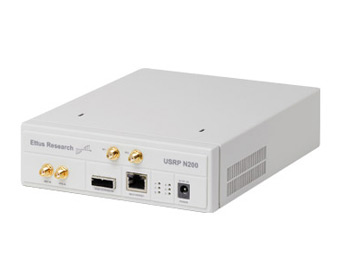
\includegraphics{Images/n200}
\isucaption{The USRP N200 from Ettus Research (Image from Ettus Research Website - www.ettus.com)}
\label{N200}
\end{figure}
}

The N200 utilizes a flexible architecture through the use of daughter-boards for a variety of RF interface systems based on the frequency range desired and if receive and/or transmission is needed.  Figure \ref{N200_block} shows the overall architecture of the N200 SDR.  These daughter boards directly receive the RF signal and then outputs the analog I and Q signals that are then sampled by the N200 A/D converter for reception or receives the I and Q values from the N200 D/A converter for transmission. 

{\begin{figure}[h!tb] 
\centering
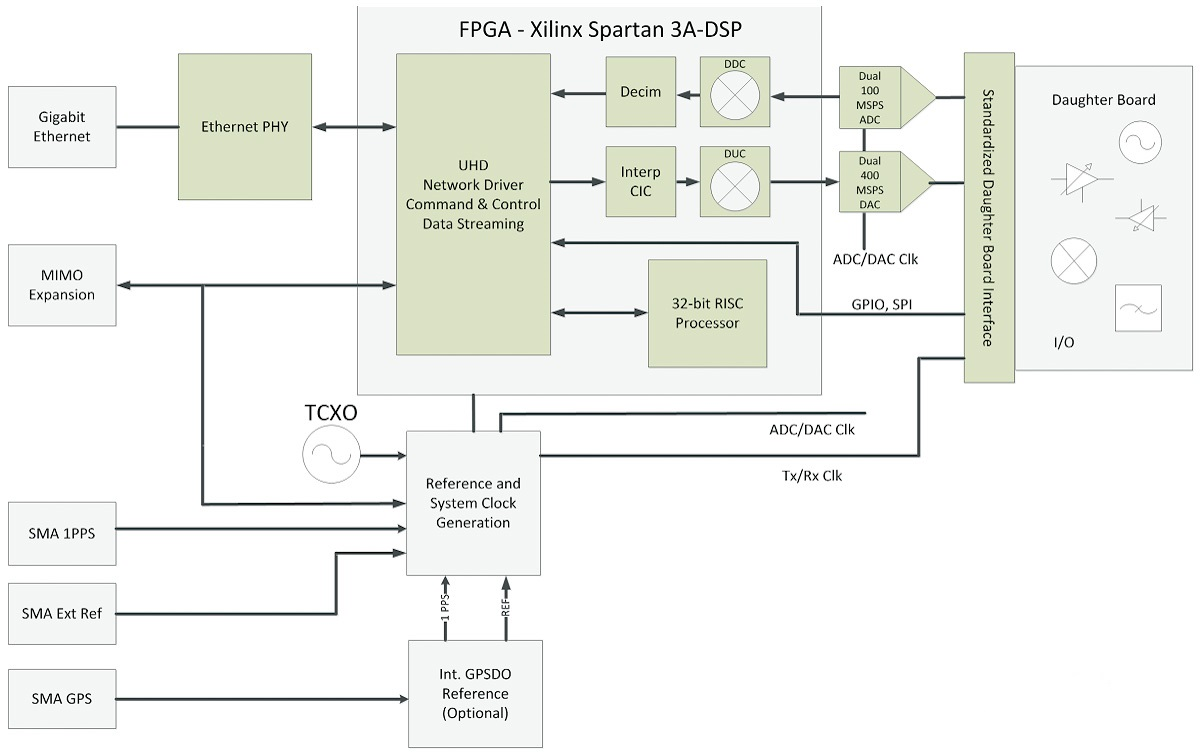
\includegraphics[width=14cm]{Images/n200_block_edited}
\isucaption{A block diagram of the Ettus N200 SDR. (Image from Ettus Research Website - www.ettus.com)}
\label{N200_block}
\end{figure}
}

The flexible architecture of the N200 and the ability for it to handle large amounts of bandwidth made this hardware ideal for the software defined radio radiometer work done in this thesis.

%These specifications had a large impact on the selection of the N200 for this application.  Specifically the 14-bit ADC, the 50 MS/s and the modular daughter-board system were the largest factors in the decision to use the N200 SDR.  Further explanation on these specifications are explained in the following sections.

%\emph{14-bit ADC.}  The analog to digital converters (ADC) allow us to take the analog I and Q values from the daughter boards and digitize this information.  Once digitized, we can now work with the signal both on the on-board FPGA board or stream it to the computer so that our software can manipulate the signal.  In radiometry, we are primarily looking at the overall power of the signal and this does not require us to accurately recreate the signal.  However, as will discuss later there are times were we do want frequency information and having an accurate frequency representation of the signal will then be an important factor.

%\emph{50 MS/s Bandwidth.}  The N200 is capable of working with up to 100 MS/s signal and can stream up to 50 MS/s through the Gigabit Ethernet connection.  The N200 also has the ability to have up to 2 daughter boards installed.  If we assume each will have up to a 20 MHz signal, this means up to 40 MS/s of data will be required.  This means that the N200 meets and can exceed the bandwidth requirements that we were looking for.  In addition, the FPGA on the N200 is capable of working with up to 100 MS/s, so there is room in handling additional bandwidth by using the on board FPGA to process the signal.

%The daughter board selected is the DBSRX2 card as this card is receive only and operates between 800 MHz and 2.4 GHz.  The DBSRX2 also has built in amplification that is adjustable through software.


\emph{The DBSRX2 Receiver.}  The daughter board selected is the DBSRX2 card as this card is receive only and operates between 800 MHz and 2.4 GHz.  An image of the daughter-board can be seen in figure \ref{dbsrx2}.  The DBSRX2 also has built in amplification that is adjustable through software.  These daughter boards have the required RF hardware for the signal to be processed.  In this application it was required that the signal was detected at 1.4 GHz with a bandwidth of 20 MHz.  The DBSRX2 receiver met this requirement and was selected to be used with the N200.  In this radiometer application transmission is not needed and is illegal in the 1.4 GHz band, which is reserved for passive radiometer applications.

{\begin{figure}[h!tb] 
\centering
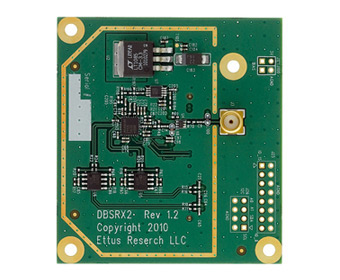
\includegraphics{Images/dbsrx2.jpg}
\isucaption{The DBSRX2 daughter board from Ettus Research (Image from Ettus Research Website - www.ettus.com)}
\label{dbsrx2}
\end{figure}
}

The DBSRX2 has several key components on it that is used to take the analog RF signal and prepare it for digitization by the analog to digital converter.  First the signal is amplified through a Programmable Gain Amplifier (PGA).  This PGA is accessible from the software and can be configured by the software.  Next the signal goes into a direct-conversion integrated circuit that directly converts the RF signal to analog I and Q values.  The integrated circuit, a Maxim MAX2112 device, also includes a Low Noise Amplifier (LNA), mixer and Low Pass Filter (LPF).  This essentially amplifies the signal, mixes into baseband and then applies a low pass filter.  

%{\begin{figure}[h!tb] 
%\centering
%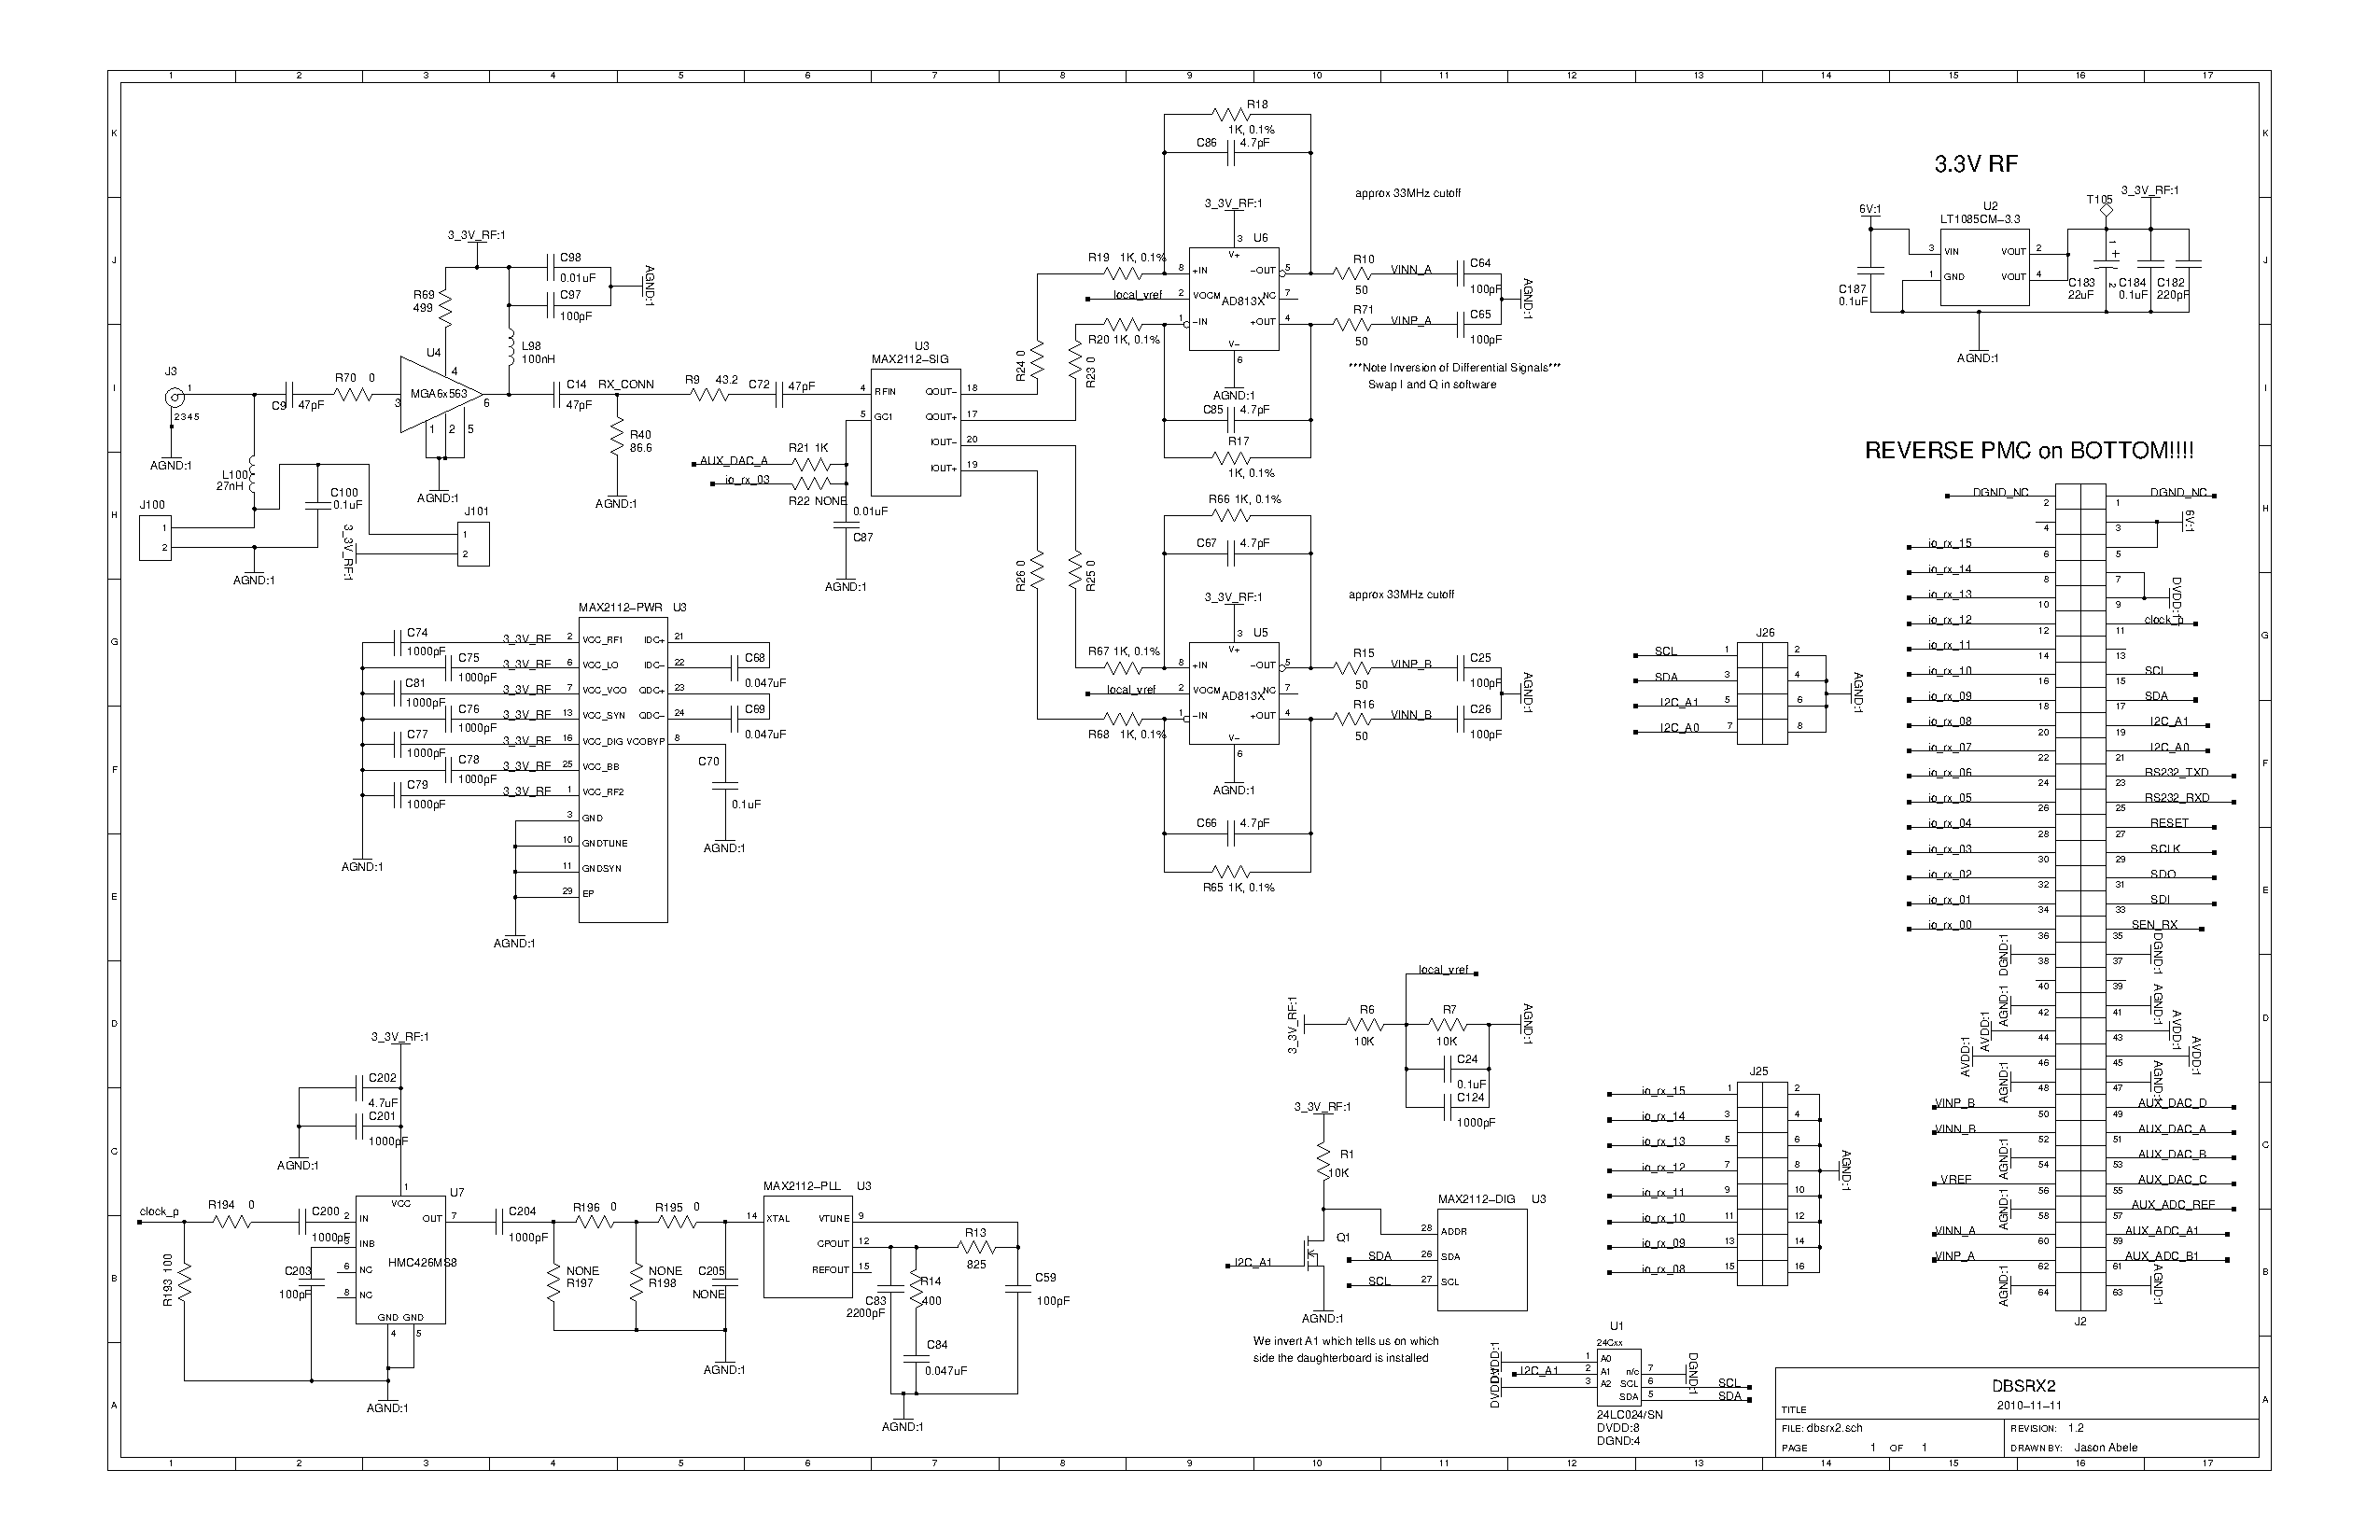
\includegraphics[width=\textwidth]{Images/dbsrx2.pdf}
%\isucaption{The DBSRX2 Schematic (Image from Ettus Research Website - www.ettus.com)}
%\label{dbsrx2_sch}
%\end{figure}
%}

These analog I and Q values are then passed to the N200 to be sampled by the analog to digital converter.  The IQ values are differential signals to minimize noise possible interference.

Since we are using the DBSRX2 after the LNAs that are already in use, the noise temperature added by the DBSRX2 will be small.  The DBSRX2 adds approximately 5 dB to the noise factor of the system.  Again though, since this is at the end of the RF chain, the total contribution of the DBSRX2 to the overall system noise temperature is small, and has been calculated to be 1.05 dB to the overall noise factor of the system.

\subsection{Software Platform} 

Software of course plays a critical role in a software defined radio and also in our software defined radio radiometer.  There are two pieces of software that are in play with the software defined radio we are using.  The first is the firmware that is used in the FPGA of the N200.  This firmware provides low level processing of the signal so it can be sent to the software located on the computer.  It also provides a link for controlling key aspects of the software defined radio such as additional gain, bandwidth and the center frequency.  This firmware is already pre-loaded into the FPGA by Ettus Research and can be upgraded through tools provided by Ettus Research.

The second is the software that is running on the host computer.  It is this software that provides the calculations on the I/Q data to give us the information we need and also creates a GUI for the user to interface with the radio.  For this software, we will be using GNURadio, an open source software program that is used in software defined radios including the N200 SDR that we have.  

GNURadio will be used to do all signal processing that is needed.  GNURadio is an open source software define radio framework that runs on multiple OSes and offers a rich set of features.  In addition, GNURadio is well supported by the Ettus Research group and is the preferred software for interfacing with their hardware.  

An easy to use interface was another driving requirement for our implementation of a radiometer in a SDR.  GNURadio helps us with this through the use of the GNU Radio Companion or GRC.  This was important as it was anticipated that operators of the radiometer have a limited knowledge about programming.  GRC uses a simple to use graphical system to design and build radio components in software.

%GNURadio  and GRC is written in Python, which allows for easy modification and access to additional tools that can be used with GNURadio.  While most of GNURadio is written in Python, C is used for any of the low level drivers and interface to the hardware.  This is done to optimize speed and performance of GNURadio.

%GNURadio fills in the software side of the software defined radio.  Although there is firmware that runs on the FPGA in the N200, this firmware is designed to communicate with a host PC.  It is this software that does most of the work by doing the calculations that apply to the signal.  The FPGA simply sends the raw IQ data to the host PC, which then performs the necessary math functions.  Again, the reason why software defined radios are desirable is the ability to change the behavior of the radio quickly.  In our scenario we can change functionality by simply loading a new software program in the host PC.  

%This functionality is ideal for communication type of radios where different modulation schemes and encoding and decoding methods can easily be changed out.  However, in a radiometer we are not interested in this aspect of the SDR.  However, one functionality is available that can be valuable for a radiometer, and that is with filtering.  Although we often use frequencies that should be free from interference, this is not always what happens in the real world.  Interference can and often does still occur, even in these protected frequencies.  With the SDR, we are able to quickly adapt to changing conditions by moving the frequency, changing our bandwidth and even filter out an offending signal.  

%GNURadio was selected as it is an open source software platform.  GNURadio is licensed under the GPL license and has a strong community that continually updates the software.  It is also well supported by third parties such as Ettus Research Group, National Instruments and other SDR developers.  In addition, GNURadio has a strong set of tools that can be used to develop programs that run under GNURadio.  Tools such as the GNURadio Companion (GRC) allows for an easy to use GUI to develop code for GNURadio.  GNURadio is also written in Python, which allows for easy modification and access to additional tools that can be used with GNURadio.  

{\begin{figure}[h!tb] 
\centering
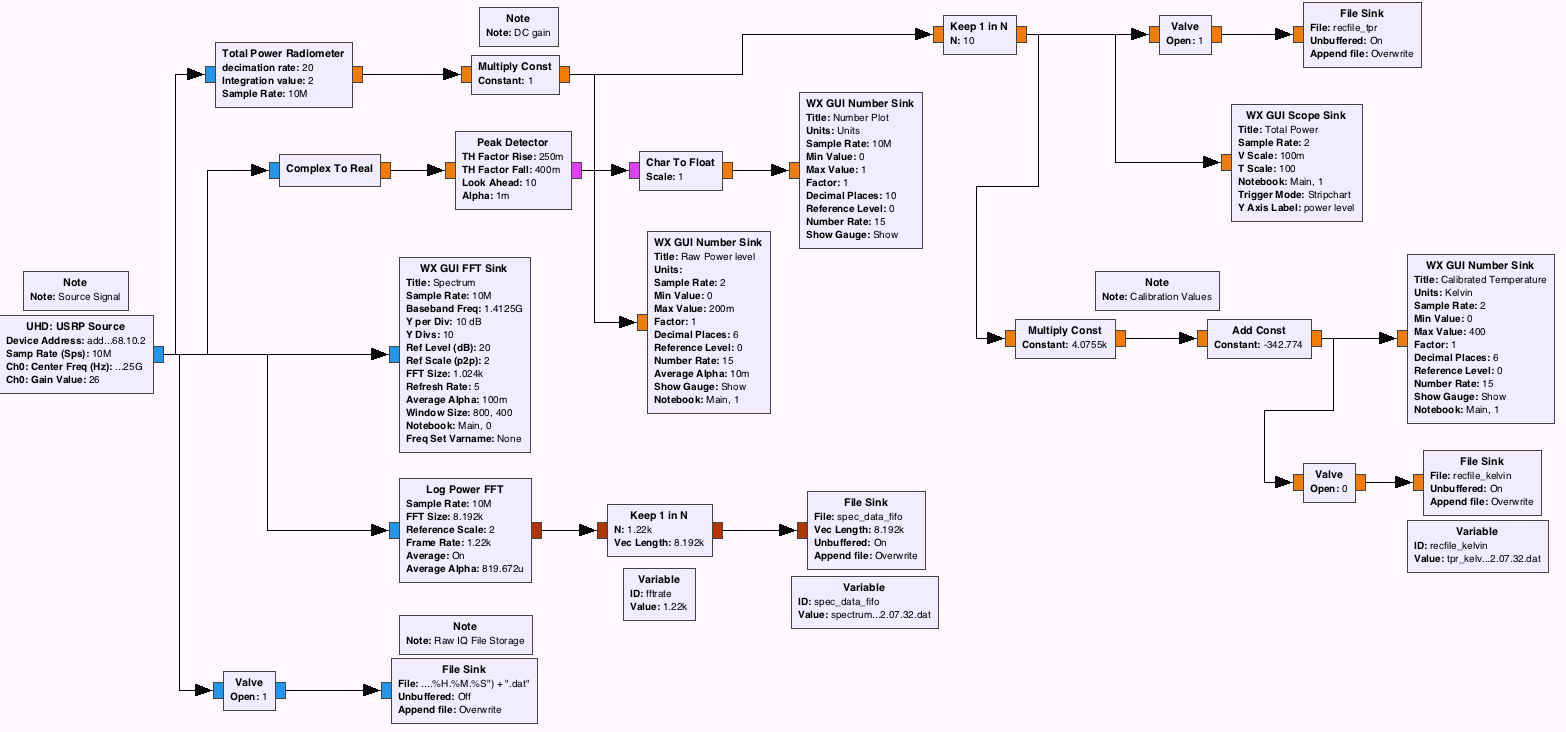
\includegraphics[width=17cm]{Images/N200_radiometer_grc.png}
\isucaption{Screenshot of the GNURadio Companion editor and the N200 Radiometer block diagram used in the author's experiments}
\label{N200_GRC}
\end{figure}
}

GNUradio Companion works by having the common functions, such as signal sources, signal processing and signal sinks, as blocks that can picked and placed on the screen.  Once placed, the blocks can be wired up, much like LabView, and the flow of data can be controlled in this fashion.  While GNURadio Companion provides most of the essential blocks used in most applications additional blocks can by added if needed.  This is because GNURadio is built using Python and the blocks in GNUradio Companion are simply blocks of Python code.  To compile a GNURadio Companion flow diagram, you simply run the sheet, which then generates the Python code that is then executed.  

GNURadio uses a combination of Python and C++, where Python handles most of the interface and the C++ is most of the drivers and low level interface to the hardware.  This allows for an easy to use system but still meets the demanding performance needed for handling large amounts of data.  

GNURadio Companion also includes blocks that allow it to create a GUI type of interface.  The typical method it uses for this is using wxGUI although GNURadio Companion does also include blocks that can use QT for generating widgets as well.  However, the wxGUI tends to work better and has better support in GNURadio than QT.  

Through these blocks we are able to only manipulate the data we need to perform a total power radiometer in software but to also create a user interface that allows us to control the radiometer as well.  We are also able to display the information in real time so the user can see changes in power and even monitor spectral information during the operation of the radiometer. 


%----------------------------------------------------------
% End of Chapter 3.  Anything below this is extra information

% Chapter 4 from the standard thesis template
% that contains an adv. example table and figure.
\chapter{SOFTWARE DEFINED RADIOMETER IMPLEMENTATION}\label{ch:implementation}

This chapter examines the implementation of a software defined radio based radiometer.  First we will examine requirements of both a traditional radiometer and a digital radiometer.  Next we will map the traditional radiometer components discussed in chapter \ref{ch:background} to their digital counterparts.  Finally a high level overview of a software defined radio based radiometer will be given.

\section{Requirements}\label{requirements}

This section discusses the hardware and software requirements used to drive the selection of the hardware and software platforms use to implement our software defined radio based radiometer.  

\emph{Hardware Requirements.}  The capabilities of existing traditional radiometers were the primary driving force in setting the requirements of our hardware development platform.  Dr. Brian Hornbuckle from the Electrical and Computer Engineering and Agronomy department at Iowa State University was consulted with respect to key specifications of his radiometer.  Additionally, the specifications of other radiometers were examined. 

Table \ref{rad_performance} summarizes the specification of three parameters that were decided upon for selecting our hardware development platform, based on our investigation.  This lead to the selection of the N200 software defined radio platform with a DBSRX2 daughter board from Ettus Research as our platform.  Section \ref{SDR_platform} provides more in depth information on the hardware used and why it was selected.

\begin{table}[h!tb] \centering
\isucaption{Required Radiometer performance}
\label{rad_performance}
% Use: \begin{tabular{|lcc|} to put table in a box
\begin{tabular}{lcc} \hline
\textbf{Parameter} & \textbf{Value} & \textbf{Units} \\ \hline
Minimum bandwidth & 20 & MHz \\
Operational frequency & 1400 - 1420 & MHz \\
$NE\Delta T$ (sensitivity) & 1 & Kelvin \\ \hline
\end{tabular}
\end{table}

\emph{Software Requirements.}  Since an objective of this work was to help make radiometers more wildly accessible to the general research and education communities, a requirement of the development software was ease of use.  Additionally, the user interfaces developed with these software tools needed to be easy to use, while providing sufficient computing efficiency for the signal processing required for radiometry.

GNURadio met the stated requirements.  It includes a supplemental software package called GNURadio Companion (GRC), which uses a graphical interface for creating a radio environment.  GNURadio and GRC are discussed in greater detail in Section \ref{software_platform}.

%Since an easy to use system was a requirement in the selection of the software.  GNURadio was selected as it includes GNURadio Companion (GRC), a supplemental program which uses a graphical interface for creating the radio environment.  GNURadio and GRC is discussed in greater detail in Chapter \ref{ch:background}, section \ref{software_platform}. 

\section{Mapping Traditional Radiometer Functions to a Software Defined Radio Based Radiometer}

The use of a software defined radio (SDR) to implement a radiometer requires mapping components of a traditional radiometer to SDR-based technology.  This section presents the mapping of three such components for implementing our SDR-based radiometer.  These components are:  1) power measurement, 2) integration, and 3) filtering.

\subsection{Power measurement}

A traditional radiometer uses a device called a square law detector to measure power.  It transforms an input signal into an output voltage whose square is proportional to the input signal power.  Figure \ref{square_law_simple} shows a simple circuit diagram.  The random noise we measure is noise that is generated due to thermal agitation in the median.  This random noise has peak values but the mean value of the noise is zero.  The square-law detector takes the peak values of this random noise and this results in the total power detected.

{\begin{figure}[h!tb] 
\centering
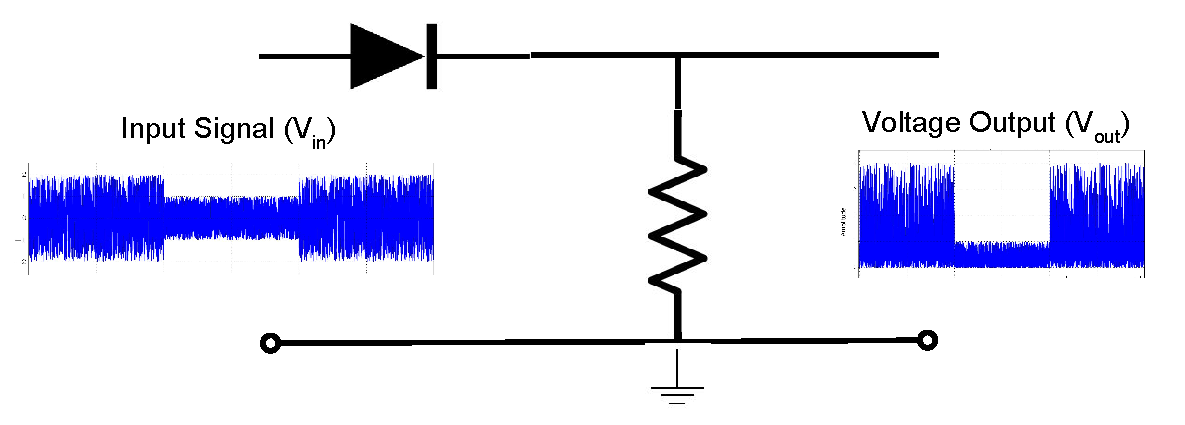
\includegraphics[width=17cm]{Images/square_law.pdf}
\isucaption{A simple diagram of a square-law detector.}
\label{square_law_simple}
\end{figure}
}

Equation \ref{sdr_x2} gives the mathematical representation of a square law detector's functionality where I is the in-phase of the input signal, Q is the quadrature-phase of the input signal, and $P_{out}$ is the power of the signal.  By squaring and summing the in-phase and quadrature phase of the signal, we obtain the magnitude of the signal which represents the power measured[\cite{Rashid}].  

\begin{equation}\label{sdr_x2}
I^2+Q^2 = P_{out}
\end{equation}

{\begin{figure}[h!tb] 
\centering
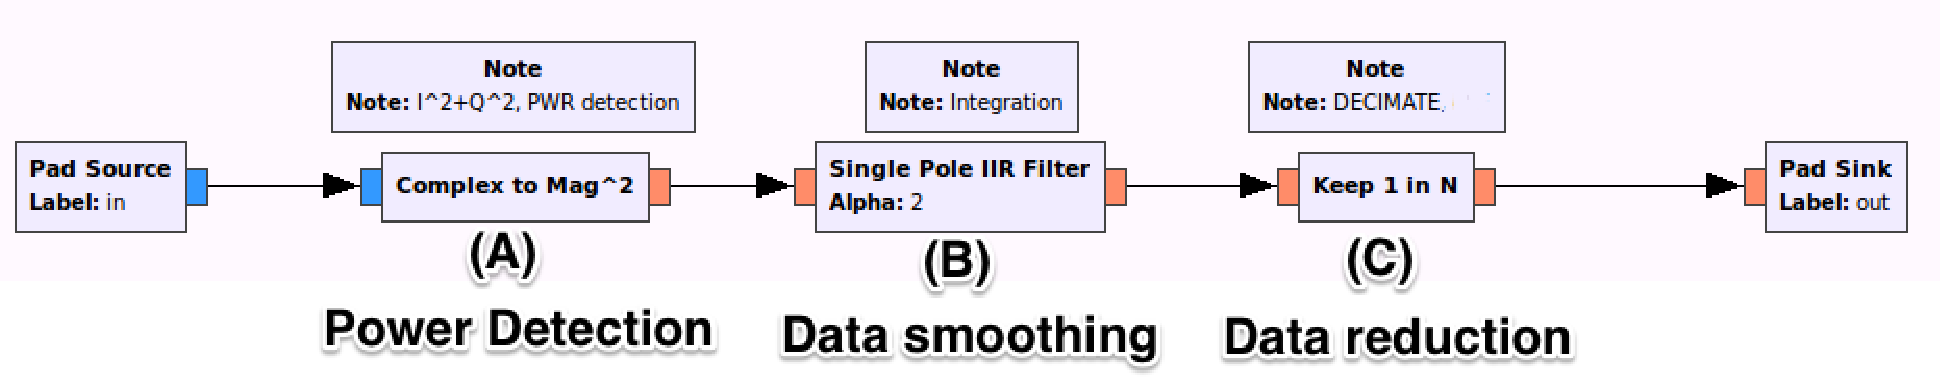
\includegraphics[width=17cm]{Images/TPR_grc.png}
\isucaption{A block diagram of the power detection, low pass filter and decimation block used for total power measurements.}
\label{square_block}
\end{figure}
}

Figure \ref{square_block} shows the block within GNURadio Companion that performs the function of total power measurement.  In Figure \ref{square_block}, the block labeled as A performs mathematically the power detection as shown in Equation \ref{sdr_x2}.  As with a traditional radiometer, this measurement will fluctuate rapidly.  Block B performs as a low pass filter to smooth the signal.  Finally block C decimates the data to reduce the sample size and thus reduce the file size of the data.  

\subsection{Integration}

A typical radiometer implement an integrator as a RC low pass filter and an IIR filter can be configured to be a low pass filter.  Output from the square-law detector is noisy due to the rapid fluctuations in the signal.  Figure \ref{square_raw} shows an example of this raw output.  This makes detecting small changes in power difficult (i.e. hinders sensitivity).  

{\begin{figure}[h!tb] 
\centering
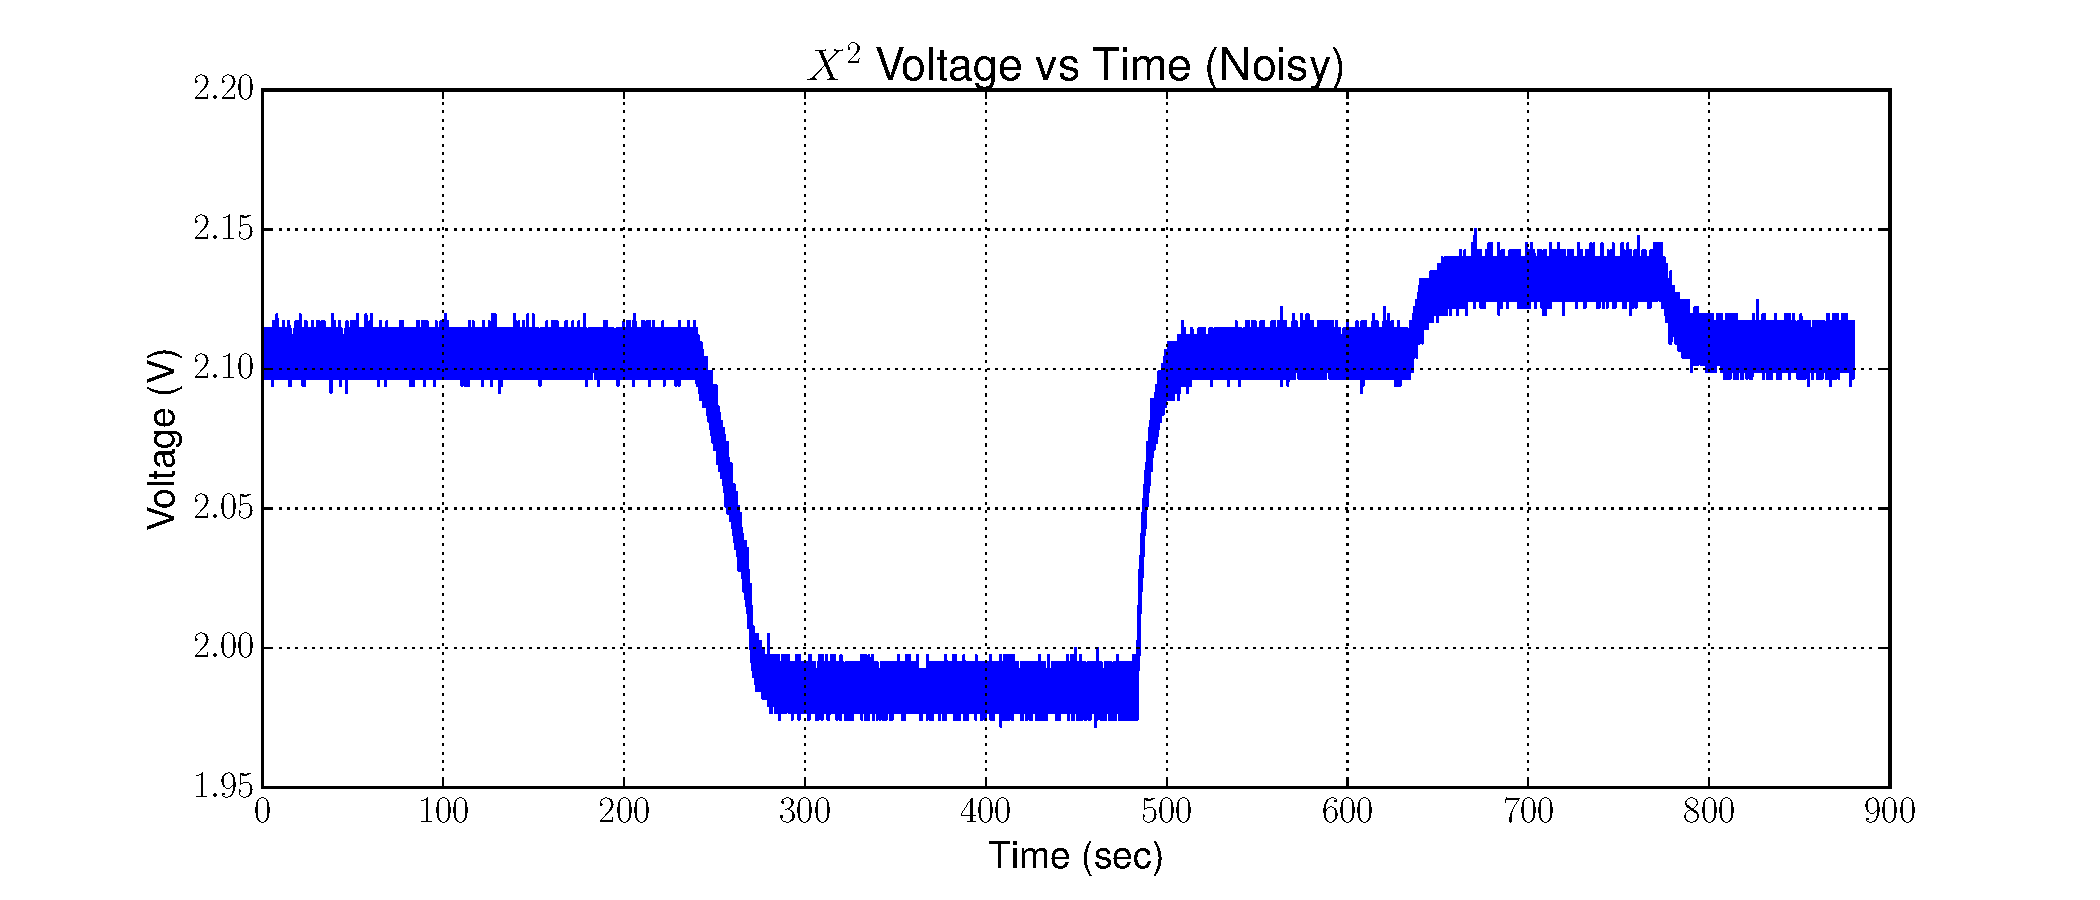
\includegraphics[width=17cm]{Experiments/Exp1/noisy_voltage.pdf}
\isucaption{Power measurements from a square law detector before filtering}
\label{square_raw}
\end{figure}
}

{\begin{figure}[h!tb] 
\centering
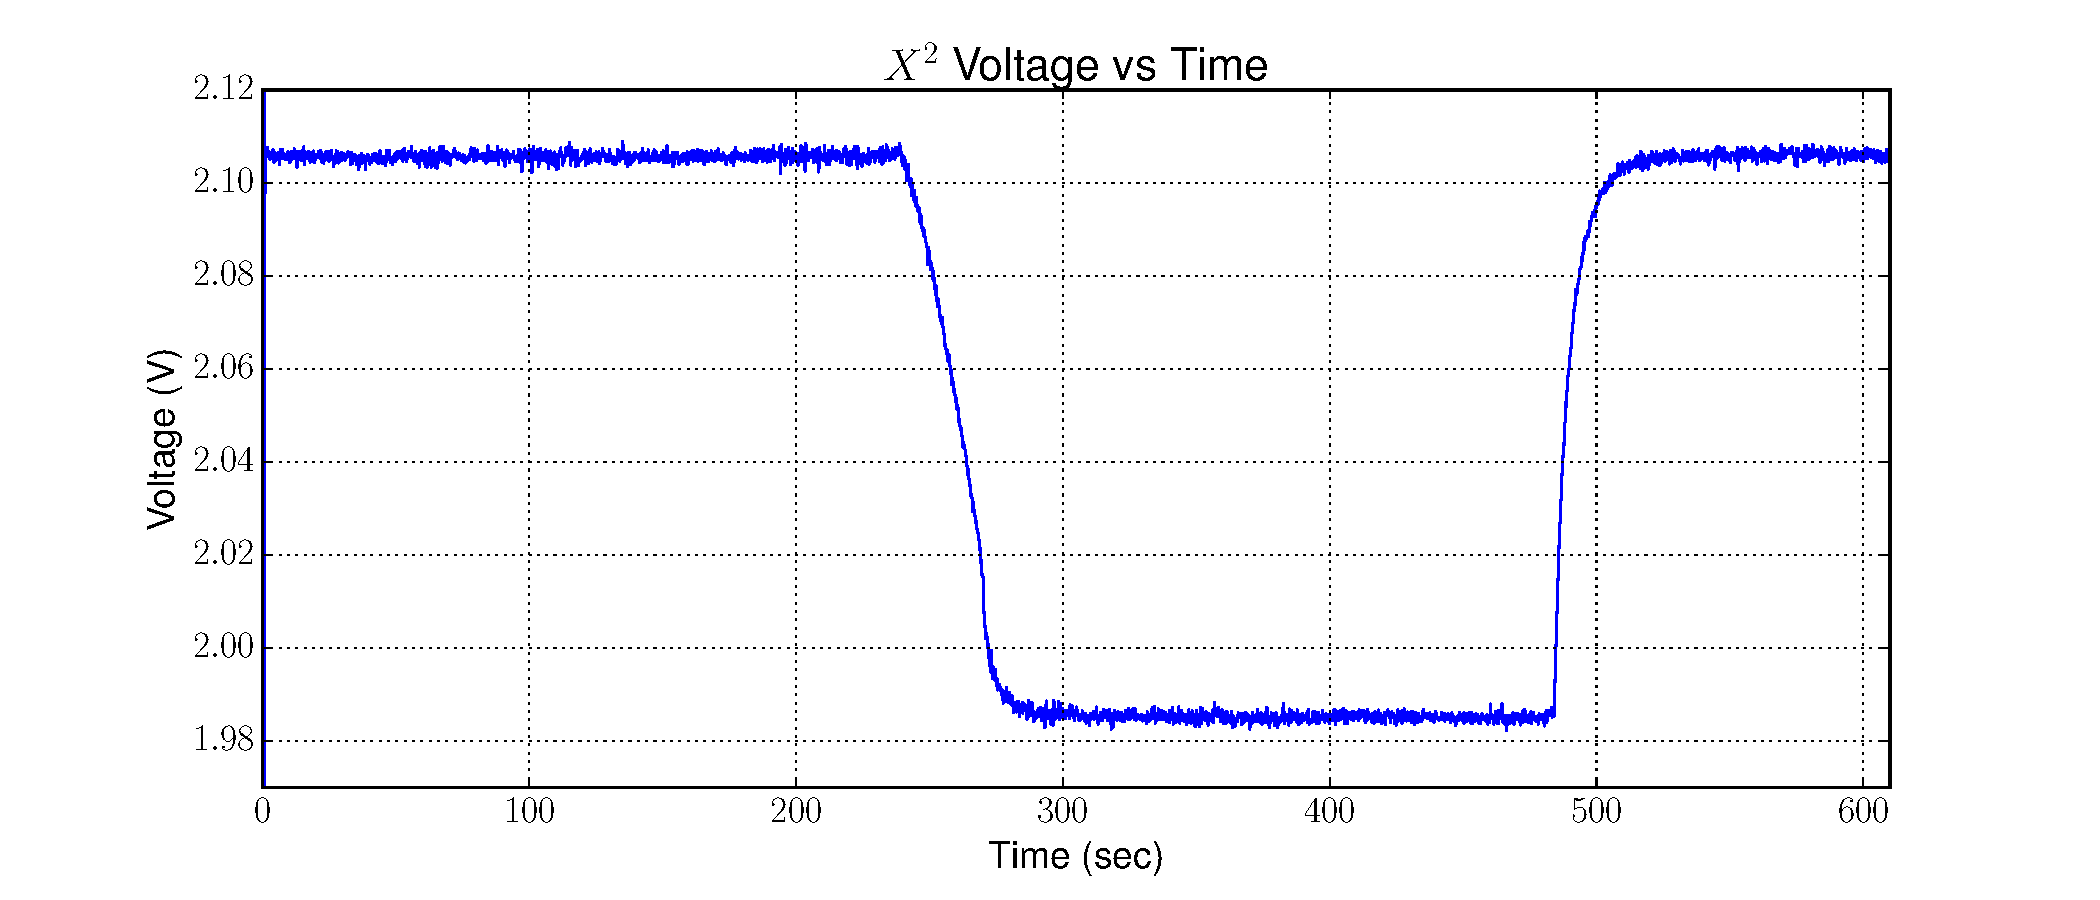
\includegraphics[width=17cm]{Experiments/Exp1/x2_filter.pdf}
\isucaption{Power measurements from a square law detector after filtering}
\label{square_raw_filt}
\end{figure}
}

%A common solution used by radiometers is to use an integrator, implemented as a RC low pass filter to smooth out this signal.   An integrator averages a signal over time, which effectively reduces the rapid fluctuations in the output.

%A traditional radiometer will use a simple Resistor and Capacitor (RC) circuit to accomplish this.  Because our signal, even a noisy one, has a frequency component, this RC circuit acts like a low pass filter.  Thus the higher frequency "noise" is filtered out.

%To improve our sensitivity, and reduce the rapid fluctuations in the power measurements, we integrate the power measurements.  This gives an average of the signal and reduces the fluctuations in the output.  This helps to improve the sensitivity of the radiometer as seen in equation \ref{NEAT_EQ}.  Chapter \ref{ch:background} section \ref{int_filt} goes in to more detail on how an analog integrator works.  The digital equivalent to a integrator is a Finite Impulse Response (FIR) filter.

To implement this low pass filter as a digital filter, an Infinite Impulse Response (IIR) filter is used.  This filter is then configured as a low pass filter that has a transfer function shown in Equation \ref{IIR_Transfer}

\begin{equation}\label{IIR_Transfer}
H(f)=\frac{\displaystyle\sum\limits_{i=0}^{P} b_i z^{-i}}{1+\displaystyle\sum\limits_{j=0}^{Q} a_j z^{-j}}
\end{equation}

%To implement this as a digital filter, a Finite Impulse Response (FIR) or Infinite Impulse Response (IIR) can be used.  A FIR filter, also known as a non-recursive filter, is a digital filter that can take an impulse signal and decays to zero after a finite number of iterations.  Equation \ref{FIR_Eq} shows the output of this filter ($y_N$) with the input $x_n$, where $P$ defines the order of the filter and is a weighted average of the most recent $P$ inputs.  The array $c_i$ holds $P$ arbitrary constants.  These values define the frequency response of the FIR filter.  

\begin{equation}\label{FIR_Eq}
y_n=\displaystyle\sum\limits_{i=o}^{P} c_ix_{n-i}
\end{equation} 

An Infinite Impulse Response (IIR) filter, also known as a recursive filter, is the same as the FIR filter, except a summation term is added which feeds back the previous output.  Equation \ref{IIR_eq} shows that a FIR filter is a IIR filter, with an extra summation term added[\cite{Cross}]. This term has the $d_j$ array which holds the weighting coefficients for feeding back the previous $y_{n-j}$ outputs.  IIR filters can produce better results with less computational cost.  However, they are harder to design and may become unstable if not designed properly.

\begin{equation}\label{IIR_eq}
y_n=\displaystyle\sum\limits_{i=o}^{P} c_ix_{n-i}+\displaystyle\sum\limits_{j=1}^{Q} d_jy_{n-j}
\end{equation}

To design either a FIR or IIR filter, the coefficient arrays $c_i$ and $d_j$ are often referred to as "taps".  These tap values define the filter as shown in Equation \ref{FIR_Eq} and Equation \ref{IIR_eq}.  To generate these tap values, GNURadio provides a filter design program.  This program is both a standalone GUI program and can also be called from within a GNURadio Companion.  The sampling rate, frequency response and cutoff frequency can be sent to the program to calculate the required taps.  

In terms of computational and memory requirements, the more taps we generate the more accurate the filter will become.  It will also be possible to design a filter with a faster (steeper) frequency response with more taps.  However, each tap requires memory for it to be stored and also requires computation against the input signal.  Therefore more taps also require more computational and memory requirements.  

%Both filters produce the same result by giving the average of the input signal.  An IIR filter however often uses less computational power than a FIR filter.  Because of this, an IIR filter was used in defining our integrator in a software defined radio based radiometer.

To get a better understanding on how the digital IIR filter relates to the RC filter analog, we need to look at the frequency response of the digital filter.  We can do that by looking at the Fourier Transform and the relationship of the input to the output in the frequency domain in Equation \ref{Fourier_IIR} where $f$ is our frequency in Hz and $T$ is our time between samples in seconds.  

\begin{equation}\label{Fourier_IIR}
H(f)=\frac{\displaystyle\sum\limits_{i=0}^{P} b_i z^{-i}}{1+\displaystyle\sum\limits_{j=0}^{Q} a_j z^{-j}}
\end{equation}

Our IIR filter needs to behave like a low pass filter to filter out the high frequency components.  As discussed earlier, an analog radiometer might do this with a simple RC circuit.  Figure \ref{rc_circuit} shows what this circuit looks like.

{\begin{figure}[h!tb] 
\centering
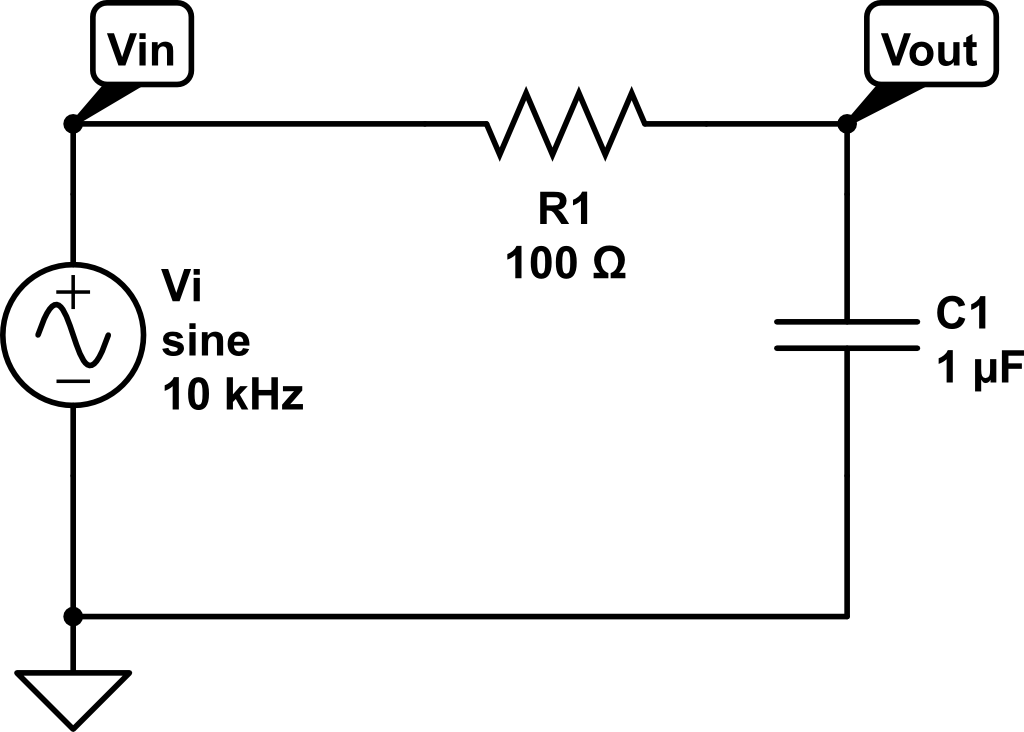
\includegraphics[width=14cm]{Images/rc-circuit.png}
\isucaption{A simple RC circuit.}
\label{rc_circuit}
\end{figure}
}

In Figure \ref{rc_circuit}, the input is $V_{in}$, the resistance value is $R$, the capacitance value is $C$ and the output is $V_{out}$.  This circuit can be represented by Equation \ref{eq:rc_circuit_eq}.

\begin{equation}\label{eq:rc_circuit_eq}
\frac{V_{in}-V_{out}}{R}=C\frac{dV_{out}}{dt}
\end{equation}

Equation \ref{eq:rc_circuit_eq} represents the differential equation relating the input voltage $V_{in}$ to the output voltage $V_{out}$.  We can substitute the input to the RC circuit ($V_{in}$) as the input to Equation \ref{IIR_eq} or $x_n$.  The output of our RC circuit ($V{out}$) can also be expressed as the output in Equation \ref{IIR_eq} which is $y_n$.  However, in order to do that we must move from the continuous domain to the discrete domain that our digital filter operates in.  This is done by showing the relationship between our sampling frequency $f_s$ and our period or time between samples, $T$ and is shown in Equation \ref{sampling_rate_eq}.

\begin{equation}\label{sampling_rate_eq}
T=time between samples=\frac{1}{f_s}
\end{equation}

We can now relate our input voltage ($V_{in}$) to the input to our IIR filter ($x_n$) by multiplying our voltage input to th our period and the number of samples, $n$. shown in Equation \ref{input_IIR} and the output voltage shown in Equation \ref{output_IIR}.

\begin{equation}\label{input_IIR}
x_n=V_{in}(nT)
\end{equation}

\begin{equation}\label{output_IIR}
y_n=V_{out}(nT)
\end{equation}

Next we rewrite our difference equation by substituting $x_n$ and $y_n$ into Equation \ref{eq:rc_circuit_eq} which results in an approximated finite difference equation shown in Equation \ref{diff_xn_yn}.

\begin{equation}\label{diff_xn_yn}
\frac{x_n-y_n}{R}=C\frac{y_n-y_{n-1}}{T}
\end{equation}

We can now solve for $y_n$ algebraically and this results in our final Equation \ref{final_IIR_RC}.

\begin{equation}\label{final_IIR_RC}
y_n=\frac{T}{T+RC}x_n+\frac{RC}{T+RC}y_{n-1}
\end{equation}

Equation \ref{final_IIR_RC} shows an IIR filter that has a frequency response that closely approximates an RC circuit.  The approximation improves as $T$ approaches zero or our sampling rate approaches infinity.

To design the filter we need to look at what our desired cut-off frequency needs to be.  For a RC filter, our resistance and capacitance define our cutoff frequency ($f_c$) and has the relationship shown in Equation \ref{fc_RC}.

\begin{equation}\label{fc_RC}
f_c=\frac{\sqrt{3}}{2\pi RC}
\end{equation}

Given our desired cutoff frequency we can determine our combined $RC$ value by rearranging Equation \ref{fc_RC} algebraically to Equation \ref{RC_fc}.

\begin{equation}\label{RC_fc}
RC=\frac{\sqrt{3}}{2\pi f_c}
\end{equation}

The $RC$ values are also referred to as the time constant of the circuit and we do not need to find the individual R and C values.  An example of how we can find the coefficients of our IIR filter, given a desired cutoff frequency of $f_c$ is shown next.  

For a low pass filter, we want a cutoff frequency ($f_c$) of 1000 Hz.  Given this and using Equation \ref{RC_fc} we can determine our time constant to be 2.757 x $10^-4$ or 275.7 microseconds.  If our sample rate is 1 MHz, then our $T$ value is 1 x $10^-6$ or 1 microsecond.  Plugging these values into Equation \ref{final_IIR_RC} results in the coefficient $c_0 = 0.0036$ and $d_1=0.9964$.  

Again, GNURadio includes a program that allows us to define our filter and it will generate the coefficients and taps needed for our filters.  Chapter \ref{ch:results} goes into more depth on this program.

%The $RC$ term gives us our time constant of the circuit and can be used to calculate out our coefficients.  We are not concerned about the actual values of R and C with our IIR filter, instead we just need the product of R and C.  


\subsection{Bandwidth and filtering}
A traditional radiometer will use filters to restrict the bandwidth of the radiometer.  For a software defined radiometer, the sampling rate defines the bandwidth for a software defined radiometer.  This sample rate may be adjusted but will be limited by the computational power available.  The higher the sample rate, and therefore the more bandwidth observed, the more computational power needed.  

Additional filtering can be created and used in a software defined radiometer.  These filters are often created using either IIR or FIR filters.  The most efficient method is to restrict bandwidth by setting the sampling rate.  However, these filters can be used to filter out either a narrow band of frequencies or to temporarily reduce the overall bandwidth.  A common application of these additional filters is to remove an offending signal detected by the software defined radio based radiometer.  This method of mitigating signal interference will be discussed in chapter \ref{ch:results}.

\section{System overview}

Like a traditional radiometer, the SDR uses an antenna to look at the target of interest.  SDRs still use an amplification to improve the sensitivity of the SDR. After that stage though, a software defined radiometer is different.  A SDR will sample and generate I and Q values that represents the signal.  From there, this data is sent to a computer to be processed.  We can then use this information to calculate the power of the signal.  In addition, we can manipulate the signal in other ways such as applying a filter to filter out an unwanted source.

%As we have shown the two of the major components of a traditional radiometer, the power detection and integration of the signal can be replicated in software and therefore can be implemented in a software defined radio.  The information can now be stored, displayed or both for further analysis.  

%There is one component of the software defined radio that we are not able to implement in software and that is with the signal amplification.  This however does play a major role in the performance of the radiometer and is a key element that should not be overlooked.  While this is not implemented in software, it still plays a critical role in our software defined radio radiometer. 

Next we will now look at how we control the software defined radiometer using the software detailed in chapter \ref{ch:background}, section \ref{software_platform} in defining the radiometer.  We will also look at how the data is displayed and stored in the software defined radiometer.

\subsection{Control of the SDR Hardware through GNURadio}
The N200 sends all data across the 1 Gbps Ethernet connection to be read in by a host computer running GNURadio.  This data is the raw I/Q values that is read by the on board A/D and processed by the on board FPGA.  An example of a very simple GNURadio software implementation would simply take this data and store the data to a hard drive in a file.  This can be very handy if we want to simply record the data and then process it later.  However, depending on the sample rate, this can consume a large amount of storage.  A short recording can  consume 1-2 GB with a sample rate of 10 Msps.  This simple system also does not give us any immediate feedback on the radiometer and it does not give us controls of the radiometer such as frequency, integration time or other key variables.  Fortunately GNURadio has tools that allows us to build up a very rich application that is able to give us the data we need and control the software defined radio as well.

The GNURadio Companion allows us to create python code that is used to not only receive the data from the SDR but also perform signal processing on the incoming information.  Additional controls are added that allow for tuning of the signal processing parameters and control of the radio functions.  With this we can build up an application that can be run on any computer that is capable of running GNURadio.  

{\begin{figure}[h!tb] 
\centering
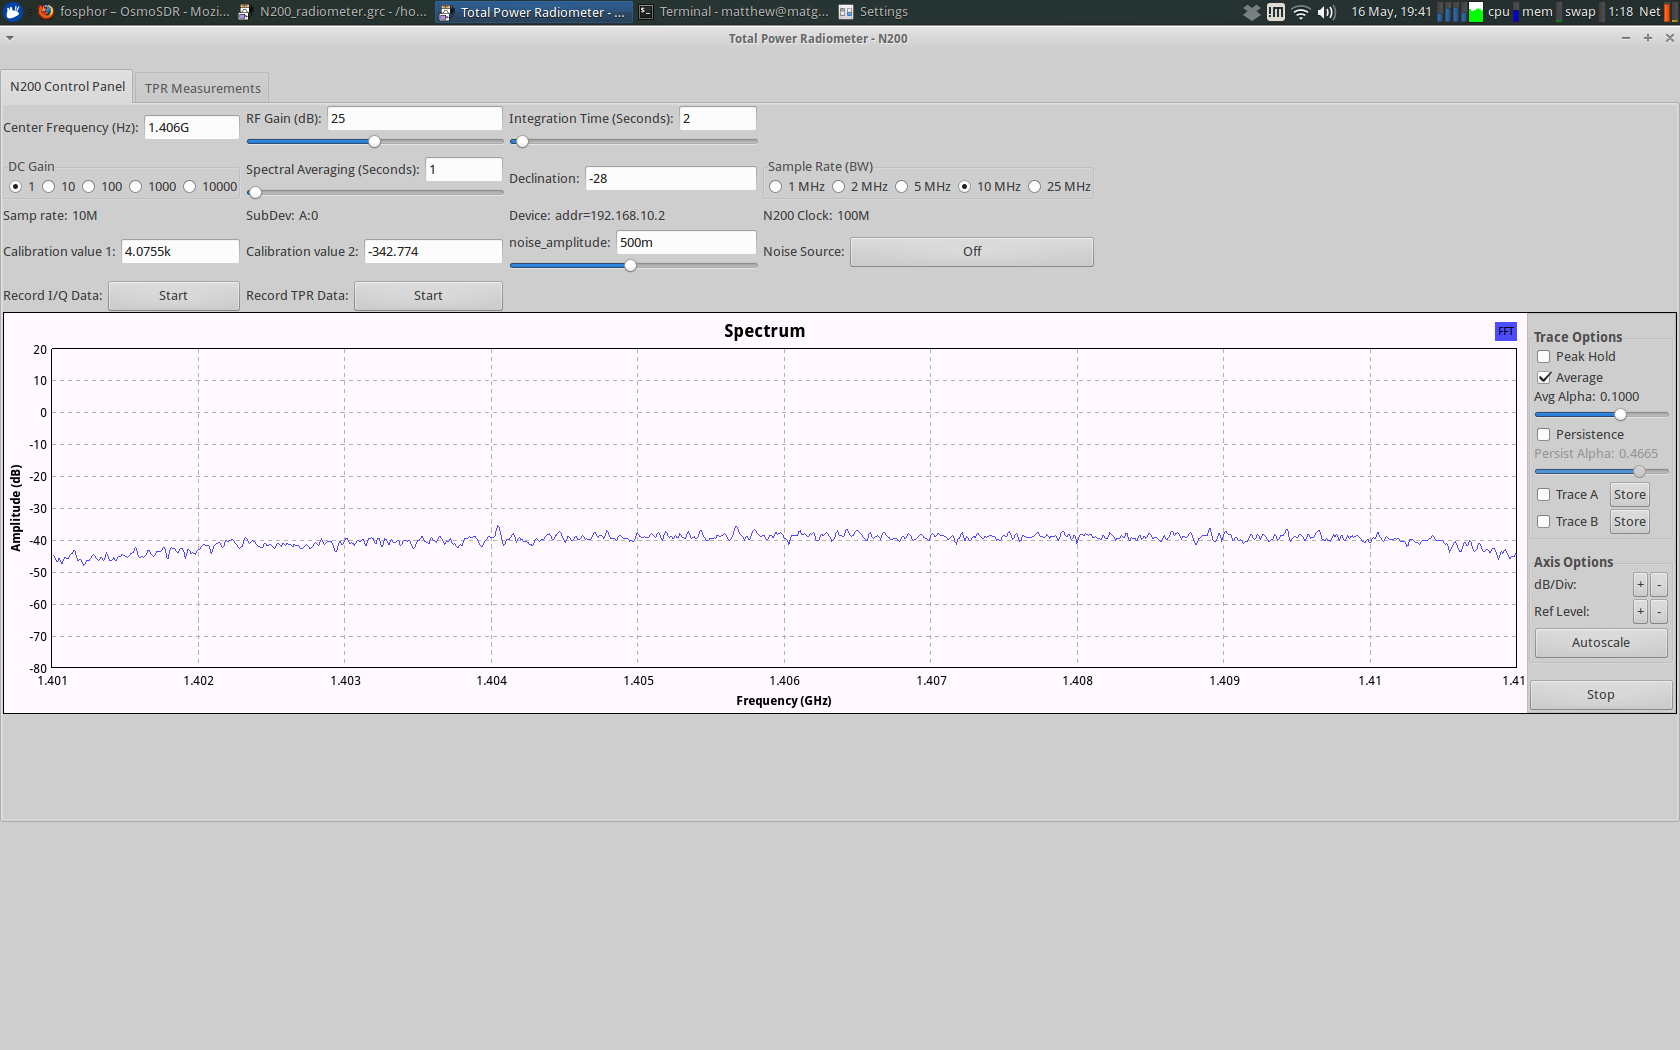
\includegraphics[width=17cm]{Images/radiometer_gui.png}
\isucaption{A screenshot of the interface made for communication with and controlling the software defined radio}
\label{radiometer_gui}
\end{figure}
}

Through this interface we are able to control several key aspects of the radio hardware within the SDR.  This has the impact of affecting the behavior of this software defined radiometer as well.  Through this we can control: frequency, sample rate (Bandwidth), integration time, and the gain on the DBSRX2 daughter board.  We will no look at how these controls impact the performance of the radiometer.  

\subsection{Impact of the Controls Related to Radiometry}

Having the ability to control these key aspects of the software defined radiometer allows us to affect the performance of the radiometer.  The $NE\Delta T$, equation \ref{NEAT_EQ}, discussed in chapter \ref{ch:background} outlines what some of these changes affect in a radiometer.

%For any radiometer noise temperature is a large consideration and is critical to the design of the radiometer.  One method to determine how well a radiometer is to look at the sensitivity of the radiometer.  We can do this by looking at the smallest change in temperature the radiometer can see.  We will call this the Noise Equivalent $\Delta T$ or $NE\Delta T$ of the radiometer and is equation \ref{NEAT_EQ} covered in chapter \ref{ch:background}.

$\beta$ can be changed by changing the sample rate of the SDR.  The sample rate effectively controls the bandwidth in which the SDR is operating at.  This also gives us a band-pass filter as well, since the SDR will not respond to frequencies outside of this bandwidth.  

$\tau$ is the integration time for the radiometer.  This parameter is set by the user through the GUI and allows us to change the integration time in seconds.

We will now look at how this data is handled and displayed by the software defined radiometer.

\subsection{GNURadio Data Handling}
Once we have the data that has been processed by the software defined radio we will want to display this information and be able to store the data so we can analyze it later if needed.  Data display is handled by GNURadio by plotting the total power over time.  This allows the user to be able to visualize the total power and be able to determine if the total power has increased or decreased over the time window shown.  

We also have the ability to look at a signal in terms of frequency versus amplitude.  This allows looking for any unusual signals that may be interfering with the system or causing erroneous data with our radiometer and is covered in chapter \ref{ch:results}.  

Finally, we will want to store the data so we can do additional analyses on it at a later time.  The GNURadio program allows us to store the data in two formats.  The first format is storing the raw I/Q data from the radiometer.  This format allows us to playback the data through GNURadio at a later time.  This can be useful for if we wish to change parameters in GNURadio such as bandwidth or integration time.  It is also a good diagnostic tool as we can check that the signal coming in is clean or if we need to apply additional filters to remove an unwanted signal.

The second format is the total power that has been calculated by the radiometer.  This file is much smaller since much of the signal information has now been reduced to simple power versus time information.  This allows for easy manipulation through any math program such as Matlab for analysis.  

\subsection{GNURadio Data Display}
The information from the software defined radio can be displayed through GNURadio to show a number of things.  Since we have both frequency and magnitude information we can display this information.  We are able to also display the information that shows the total power that is being seen by the radiometer as well.

{\begin{figure}[h!tb] 
\centering
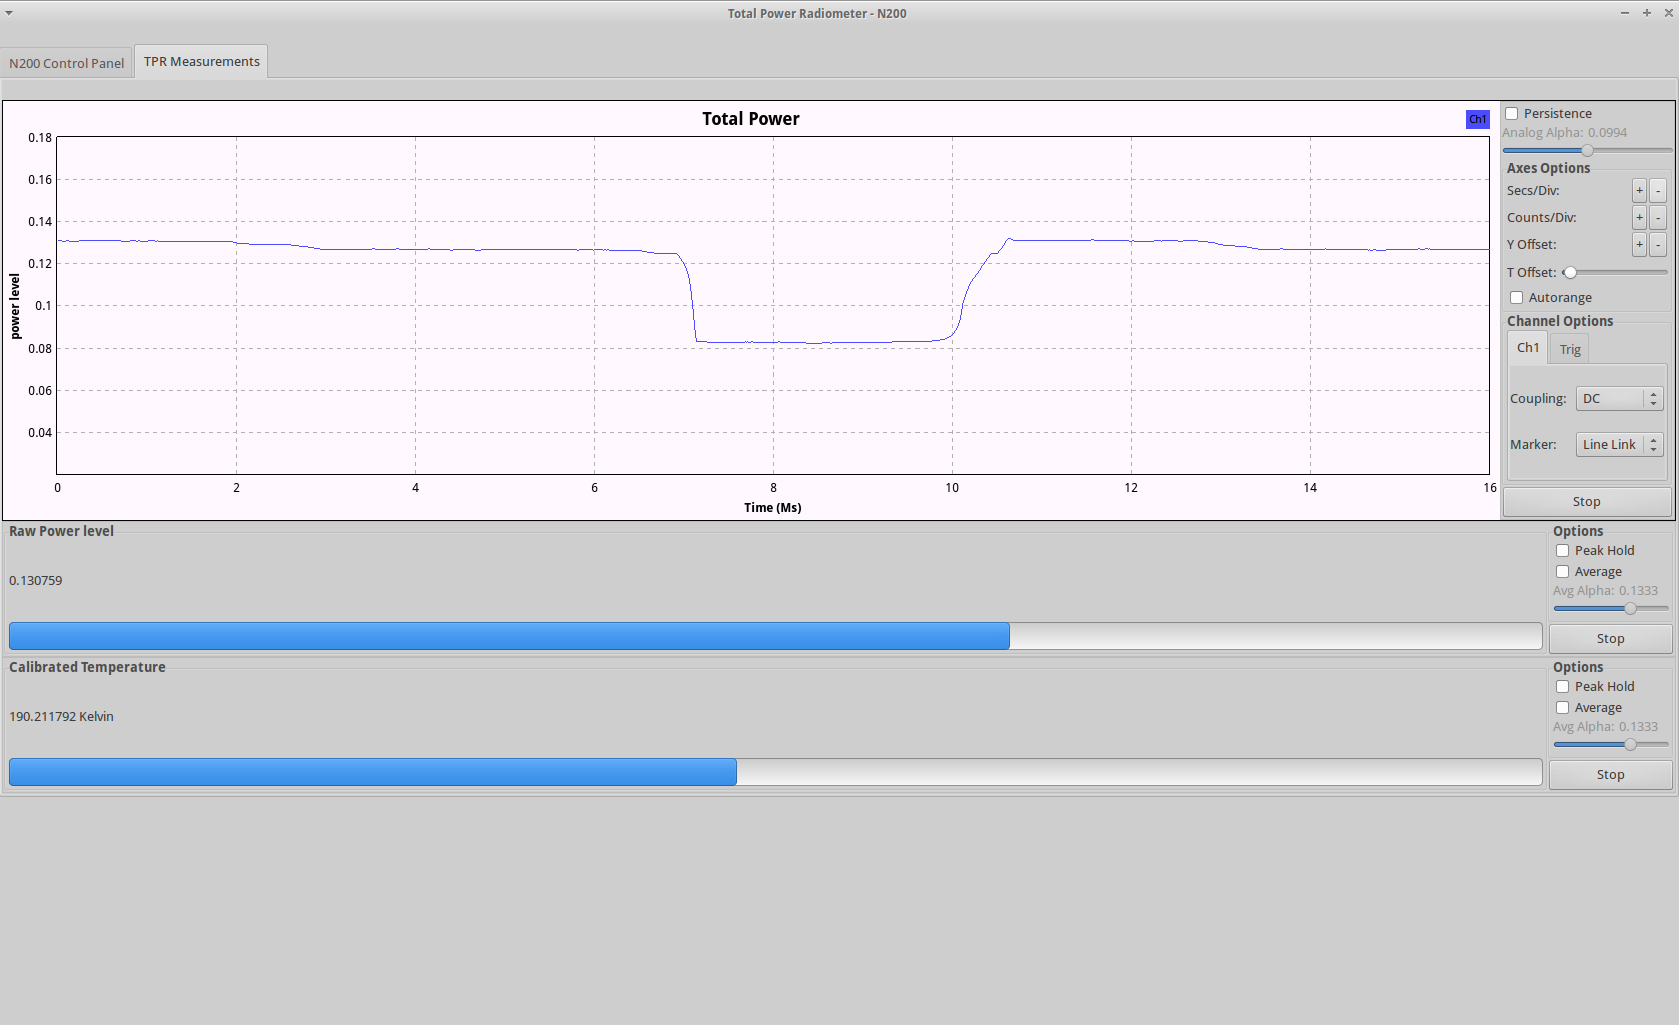
\includegraphics[width=17cm]{Images/Lab1_TPR_at_end_exp.png}
\isucaption{A screenshot showing the ticker tape display for the total power readings.  In addition, raw and calibrated noise temperature is shown below.}
\label{radiometer_tpr_display}
\end{figure}
}

We are not limited to just total power from the radiometer.  If the radiometer has been calibrated, those calibration points can be entered and GNURadio can calculate the calibrated noise temperature.  Additional information may also be added as needed.  For example, we are able to view the full spectrum that the radiometer sees.  This can be a useful tool for looking at potential RFI issues.  
%----------------------------------------------------------------------------------
%Everything below this needs to be moved/shifted or deleted

%\section{Square-law Detector Performance}
%The Square-law detector was added to our system in order to give us another reference point and to help verify the power output that the software defined radio.  Performance of our square-law detector is based on two items; the sensitivity of the diode used in the square-law detector and the analog to digital converter used to convert the analog voltage to a digital value.  The sensitivity of this device accounts for most of the performance factor of the system.  In our system the output of this square-law detector is then feed directly into an analog to digital converter.  Therefore, the performance of this A/D converter needs to be accounted for as well [\cite{Terlep}].  

%For our square-law detector, it has a noise output of $25nV/ \sqrt{Hz}$ at 100 kHz and will detect a signal as low as $-60$ dBm.  This works will with our needs since the RF front end brings the noise floor to approximately $-30$ dBm.

% Chapter 5 from the standard thesis template
%   with a full page figure and a sideways table.

%Chapter 5 will look at the results from the experiments and how the performance of the new software defined radiometer measured up.

\chapter{RESULTS AND ANALYSIS}

Radiometers measure power and it is this information that we can use to determine information about a certain target.  This power however is often expressed in terms of an equivalent temperature and if we are looking at an object, this is the brightness temperature of that object.  The primary function of the radiometer is to measure the power that is seen at the radiometer's antenna.  Ideally this is the brightness temperature of an object of interest.  In our case, this is usually looking at the ground or soil sample.  Thus the goal of the radiometer is to measure this antenna temperature with sufficient resolution and accuracy that a correlation can be made between the antenna temperature and the object's temperature that we are studying.

\section{Performance of a radiometer}
The performance of a radiometer can be measured by looking at both the sensitivity and the accuracy of the radiometer.  In addition, we need to be concerned with the stability of the radiometer as this affects the accuracy of the radiometer.


\subsection{Sensitivity}
Sensitivity of the radiometer relates to the amount of power that the radio selects from the antenna.  This selection is then dependent on the bandwidth that the radiometer is able to listen to.  The radiometer however detects not only the signal of interest but also receives a noise signal as well.  This noise is added to the signal and can not be separated from the signal.  Because this noise is added to the signal, we must be able to determine a change in the signal while the noise signal is also present.  

Power from the radiometer can be expressed in equation \ref{eq:final_power} from chapter 2, where we take into consideration bandwidth, gain and the input from the antenna plus the noise added from the antenna.  

Sensitivity relates to being able to distinguish one signal from the other.  In other words, we must be able to distinguish, or detect, our wanted signal from noise that is present in the signal.  To demonstrate this, consider a system that has a system noise temperature of 700K and an antenna temperature of 300K.  This gives us a total noise temperature of 1000K.  Therefore, if we wish to detect a change of 1K, we need to be able to detect between 1000K and 1001K.

Since our signal is really random fluctuations about a mean power input to our system, we can reduce the fluctuations by averaging or integrating the signal.  This results in equation \ref{eq:rad_sensitivity} which is derived in chapter 2.

\begin{equation} \label{eq:rad_sensitivity}
\Delta T=\frac{T_{A}+T_{N}}{\sqrt{\beta * \tau}}
\end{equation}


This equation gives us the radiometer sensitivity based on the input, which is both the noise and input signal with consideration to the bandwidth and integration time, or averaging, that is done to the signal.  

\subsection{Accuracy and Stability}
Stability and accuracy are additional problems that need to be considered when looking at the radiometer system.  To begin we can once again look at the power received equation that we discussed in Chapter 2 and is equation \ref{eq:final_power}.

As we look at this equation, we can see that if k, B, G, and $T_{N}$ are constant, then stability can be assured.  k is a known constant and we can also assume that our bandwidth, B, will also remain constant, or at least while we are taking our measurements.  Gain and the noise temperature however can vary.  

Gain is usually our largest factor that can change on a radiometer and even with a software defined radio this is still a large source of variation.  This is due to the analog nature of the amplifiers that affect a large portion of the gain in our system.  Various things can affect our gain, but the two largest factors is the physical temperature of the amplifier and the voltage that feeds the amplifier.  Voltage can be controlled to a degree.  High accuracy voltage regulators can help control fluctuations in voltages that can in turn affect the gain.  A factor however that is harder to control is temperature.  It is because of this that the current ISU radiometer has gone to great strides to control the temperature of the amplifiers to maintain a constant temperature.

\section{Required Performance Requirements}

To help us quantify the required performance of the radiometer, we referred to information provided to us by Dr. Brian Hornbuckle but also derived from existing radiometers.  As stated earlier, although a radiometer measures power, we often convert this to an equivalent brightness temperature.  Specifically, we are looking at the brightness temperature of the antenna added to the brightness temperature of the object of interest.  We also have to be able to detect a minimum amount of power.  Since changes in noise can be small, the better the sensitivity of the radiometer, the better we can detect these small changes.  

The requirements given are outlined in the table below.

\begin{table}[h!tb] \centering
\isucaption{Required Radiometer performance}
\label{rad_performance}
% Use: \begin{tabular{|lcc|} to put table in a box
\begin{tabular}{lcc} \hline
\textbf{Parameter} & \textbf{Value} & \textbf{Units} \\ \hline
Minimum bandwidth & 20 & MHz \\
Operational frequency & 1400 - 1425 & MHz \\
$NE\Delta T$ & 1 & Kelvin \\ \hline
\end{tabular}
\end{table}

\section{Square-law Detector Performance}
The Square-law detector was added to our system in order to give us another reference point and to help verify the power output that the software defined radio.  The performance of our square-law detector is based on two items.  The first is the actual square-law detector itself.  The sensitivity of this device accounts for most of the performance factor of the system.  In our system the output of this square-law detector is then feed directly into an analog to digital converter.  Therefore the performance of this A/D converter needs to be accounted for as well [\cite{Terlep}].  

For our square-law detector, it has a noise output of $25nV/ \sqrt{Hz}$ at 100 kHz and will detect a signal as low as $-60$ dBm.  This works will with our needs since the RF front end brings the noise floor to approximately $-30$ dBm.


\section{Software Defined Radio Performance}
Performance of the software defined radio is governed by the system that takes in the RF signal and then digitizes the signal.  Once the signal is in digital form, we no longer are concerned about loss of performance due to additional noise that may get added to the system.  For this reason, we attempt to digitize the signal as soon as possible.

For the N200 this is done by the DBSRX2 daughter-board that plugs into the N200 base system.  While this board does play a part in the overall system performance, because this sits later in the chain however the impact to the performance is low as shown in equation \ref{noise_factor}.  However, this module does need to be in the frequency range of the radiometer, or in our case 1.4 GHz.  This board meets that criteria.  Ideally, we still want the noise figure on this board as low as possible, even though the impact is low.  The DBSRX2 does meet this having a noise figure of approximately 5 dBm.

%Chapter 6 will look at the results from the experiments and how the performance of the new software defined radiometer measured up.

%Chapter 6: Results and Analysis

%Intro paragraph.
%Experiment 1
%	Data collected.
%	Analysis of data: Interpret the data, what was learned from the data
%Experiment 2
%	Data collected.
%	Analysis of data: Interpret the data, what was learned from the data
%Experiment X
%	Data collected.
%	Analysis of data: Interpret the data, what was learned from the data
%Price/Weight/Quality analysis (Traditional Radiometer vs. Software Defined Radiometer)
%Summary paragraph, the summary paragraph the summarized the analysis of the results.

\chapter{RESULTS AND ANALYSIS}\label{ch:results}
This chapter will display the results obtained from the experiments outlined in Chapter \ref{ch:exp_design}.  We will then give an analysis of the data included data interpretation and the information learned from each experiment.  Next we will do an analysis of a traditional radiometer vs our software defined radiometer in terms of price, weight, and quality.  Finally we will summarize our results and analysis from this chapter.

\section{Experiment I - Software Defined Radiometer Verification and Calibration} \label{Exp1_results}
As outlined in Chapter \ref{ch:exp_design}, Section \ref{Exp1}, this experiment is to verify the operation of a software defined radiometer.  This is done by performing experiments that are similar to verification and calibration methods used on a traditional radiometer.  By comparing these results to a square-law detector, receiving the same signal, we can verify the operation of the software defined radiometer.

\subsection{Data Collected}

The first data we will look at with be with the software defined radio.  The SDR records the total power measurements to a binary file that either Matlab or Python can read.  In our results, we used iPython Notebook to read and generate the graphs used in this thesis.  We will begin by looking at the raw total power readings which we will call raw Q values or rQ values.  These are the uncalibrated total power readings from the software defined radio.  

\begin{figure}[h!tb] \centering

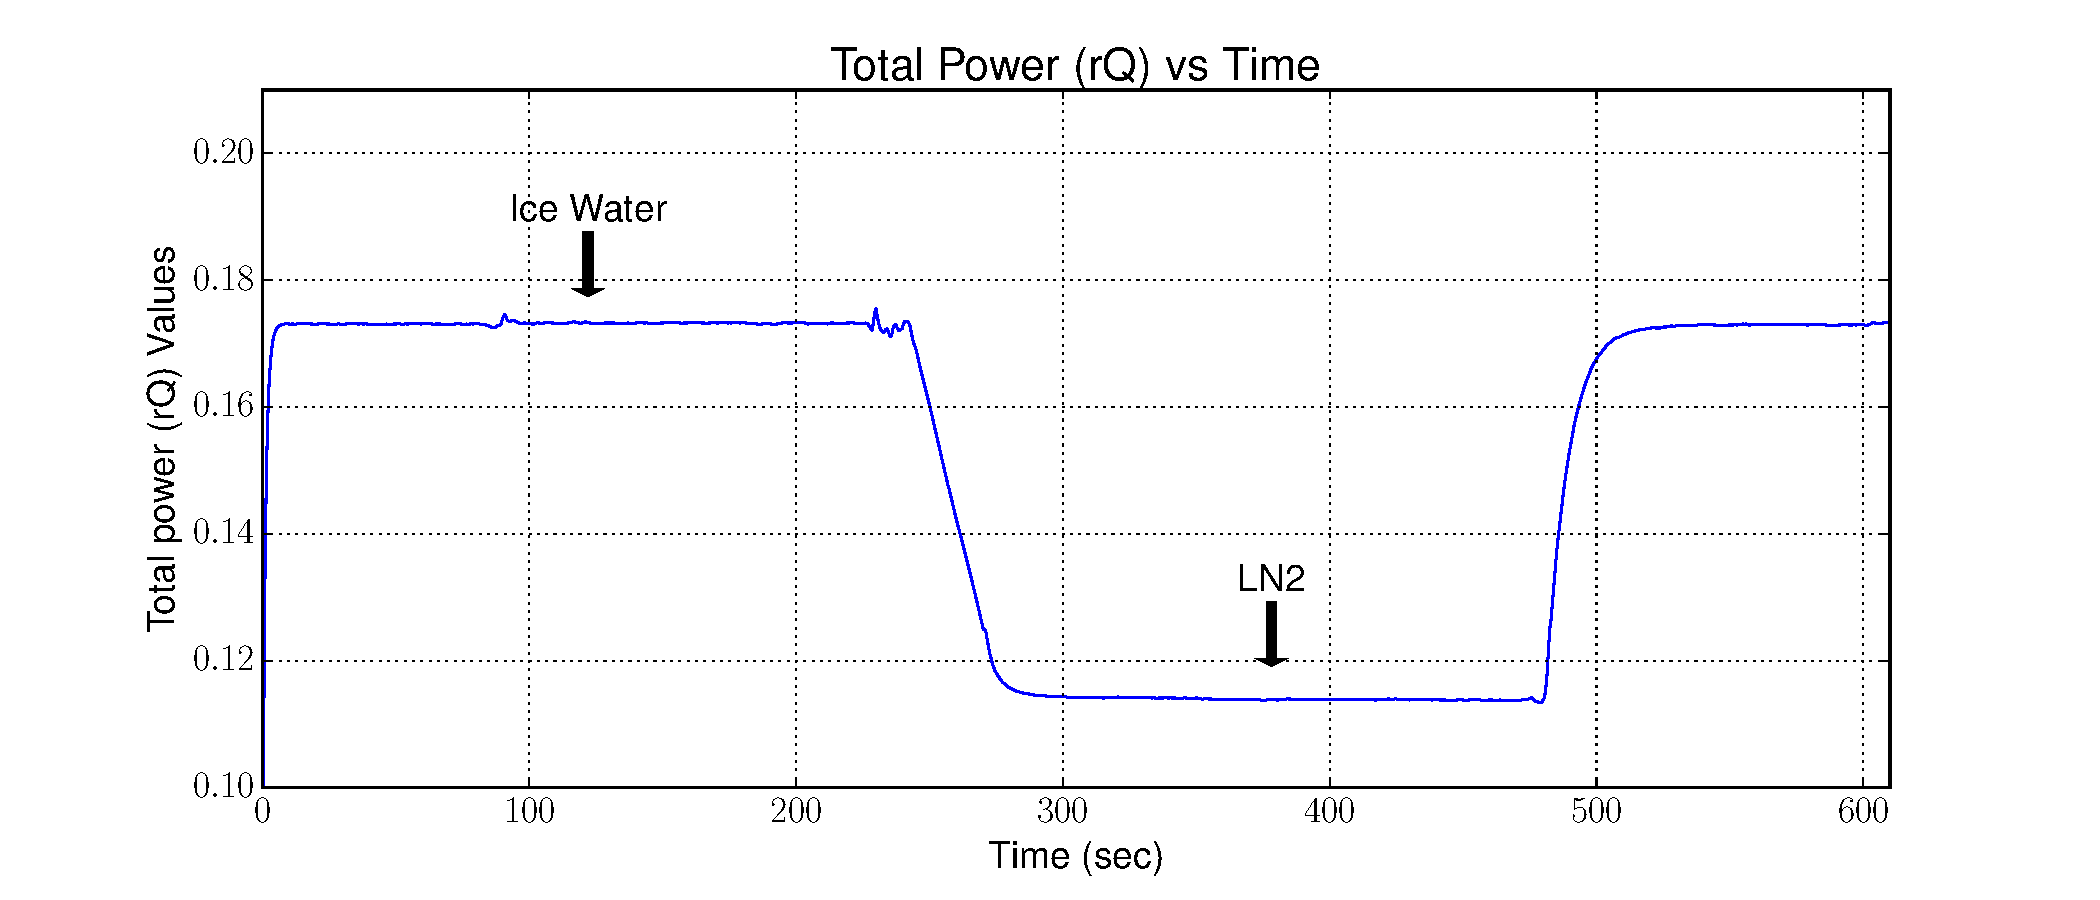
\includegraphics[width=\textwidth]{Experiments/Exp1/rqvstime_annotate.pdf}

\isucaption{Graph of the un-calibrated rQ values of Experiment 1}
\label{SDR_rQ}
\end{figure}

Figure \ref{SDR_rQ} shows the total power reading versus time and is also marked when the matched load was submerged in Ice Water, LN2, or a hot water bath.  Since we know what the temperatures are for the ice water and LN2, we can now calibrate these readings to a noise temperature reading.  This is done by reading in a calibration file we have stored in csv format and performing linear algebra to solve the slope of the line.  This was done in our iPython Notebook using the following code.
\lstset{language=Python}
\begin{lstlisting}[frame=single,keywordstyle=\color{blue}]
a = numpy.array([[rQ_values[0],1.0],[rQ_values[1],1.0]],numpy.float32)
b = numpy.array([temp_values[0],temp_values[1]])
z = numpy.linalg.solve(a,b)
\end{lstlisting}

Now that we have our calibration points, we can now re-graph this data but now calibrated as a reference noise temperature. Figure \ref{SDR_Calibrated} shows a calibrated graph of the data in relation to noise temperature.  In addition, we have colorized this graph to show warmer to cooler temps.  This is helpful as we often refer to these as noise temperatures.

\begin{figure}[h!tb] \centering

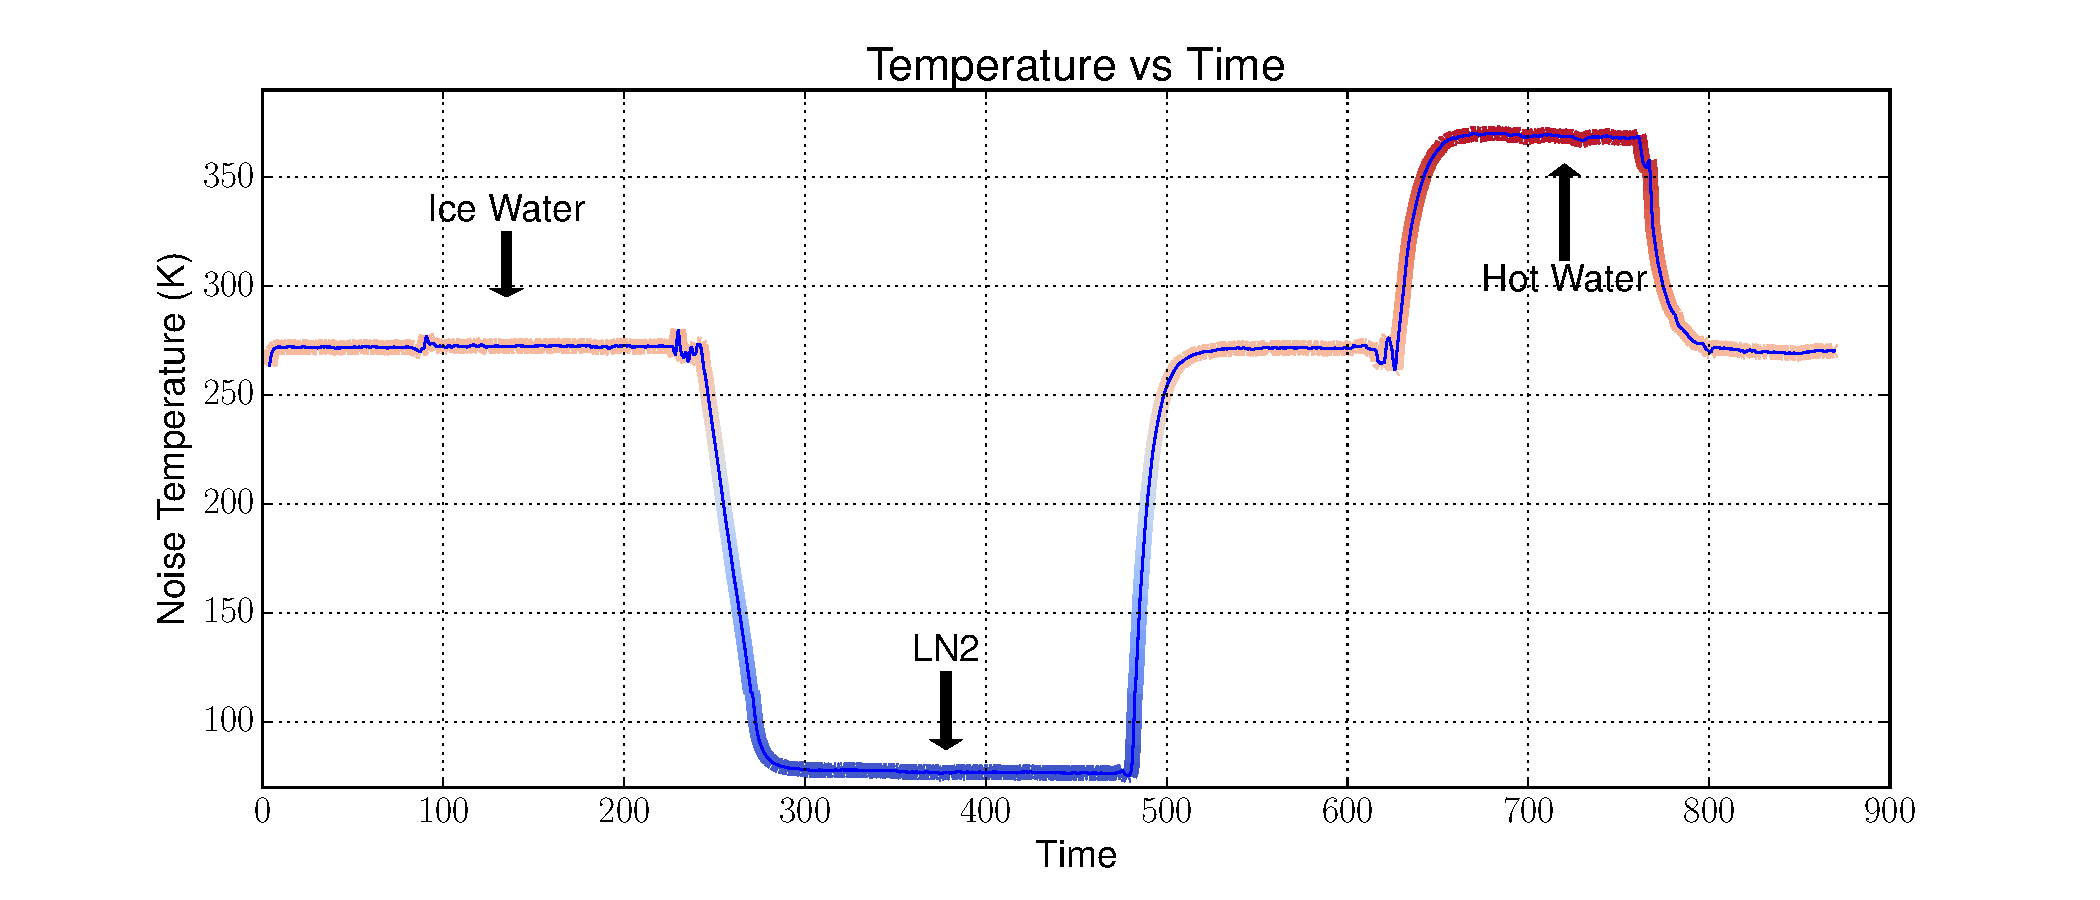
\includegraphics[width=\textwidth]{Experiments/Exp1/sdr_calibrated_color.pdf}

\isucaption{Graph of the calibrated noise temperature of Experiment 1}
\label{SDR_Calibrated}
\end{figure}

Now that we have looked at the software defined radio data, we want to look at the square-law detector with the end result of comparing the two.  The square-law detector gives us power information as a voltage, so once again we will need to calibrate this to the known temperature references.  However, before that we need to do one other step with the data.  Unlike the software defined radio, there is no filter or integrator to help smooth out the data, so the square-law data is very noisy.  Our first step will be to filter the data.  Figure \ref{X2_Raw} shows our raw data that we get from the square-law detector.

\begin{figure}[h!tb] \centering

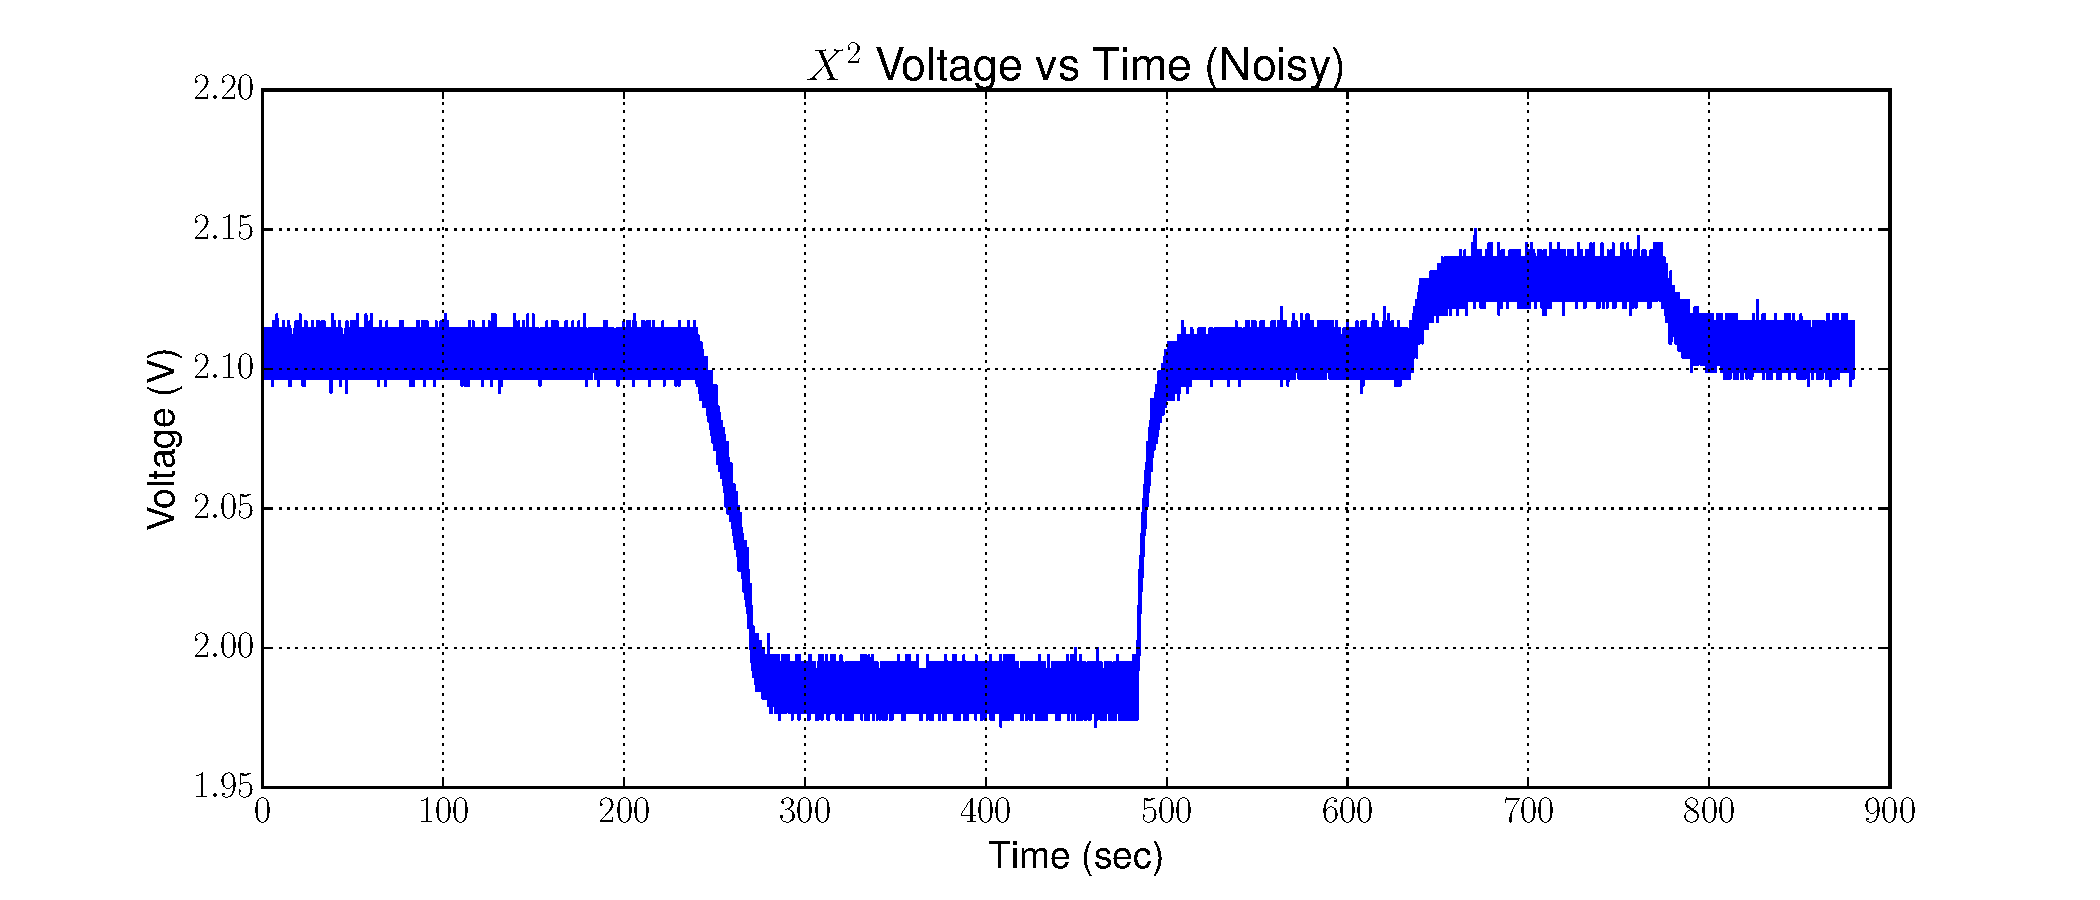
\includegraphics[width=\textwidth]{Experiments/Exp1/noisy_voltage.pdf}

\isucaption{Raw and noisy graph from the square-law detector used in Experiment 1}
\label{X2_Raw}
\end{figure}

Once again we can use Python to process this information and specifically we can use SciPy which includes several useful signal processing modules.  For our use, we will use a low pass filter to clean up the signal.  The following code allows us to do just that.

\begin{lstlisting}[frame=single,keywordstyle=\color{blue}]
from scipy import signal
N=100
Fc=2000
Fs=1600
h=scipy.signal.firwin(numtaps=N, cutoff=40, nyq=Fs/2)
x2_filt=scipy.signal.lfilter(h,1.0,x2_voltage)
\end{lstlisting}

Figure \ref{X2_filter} now shows our data that has been filtered by the low pass filter.  This is similar to the low pass filter that is also used by the software defined radio.

\begin{figure}[h!tb] \centering

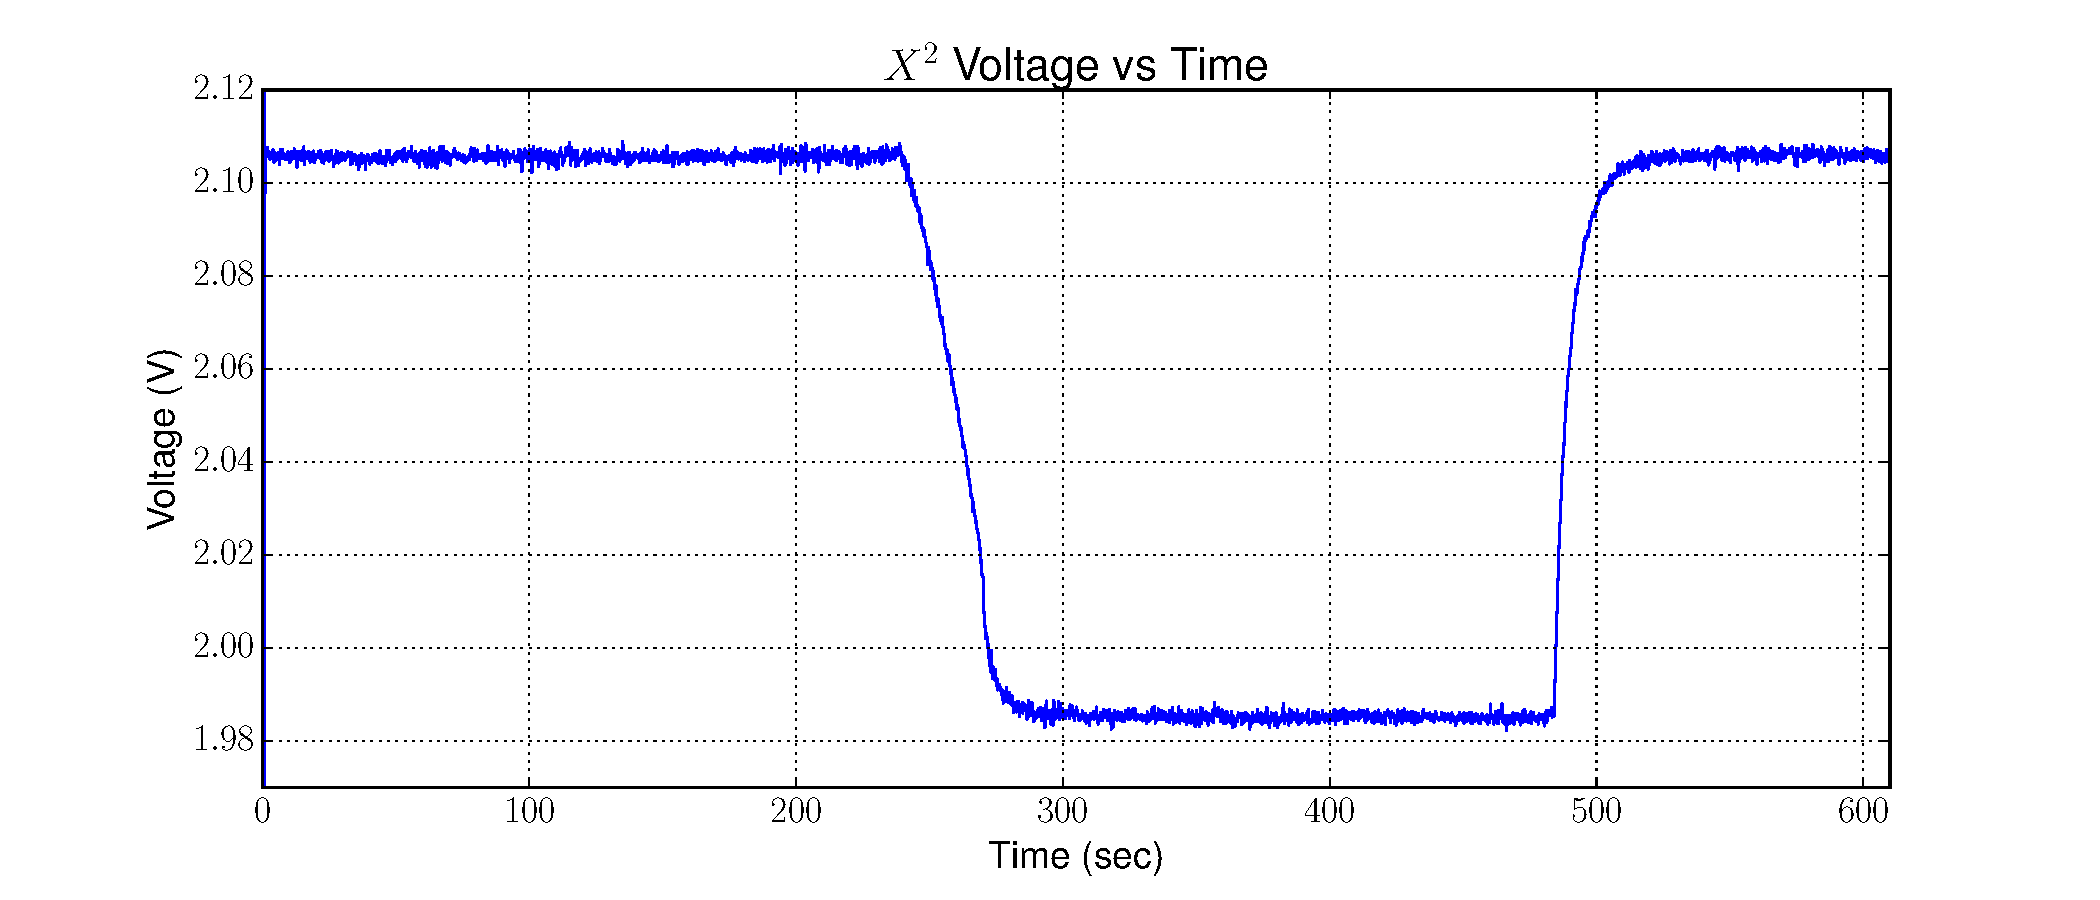
\includegraphics[width=\textwidth]{Experiments/Exp1/x2_filter.pdf}

\isucaption{Filtered data from the square-law detector used in Experiment 1}
\label{X2_filter}
\end{figure}

Using the same technique as earlier, we can now calibrate the raw voltages from the square-law detector to the noise temperature.  Like the software defined radio data, we can calibrate the voltages from the square-law detector to the physical temperature that our matched load is placed in.  Figure \ref{X2_Calibrated} shows the data from the square-law detector calibrated to our known temperature points.  This now allows us to directly compare the square-law detector to the software defined radio data since we have a common reference point in which to compare the data.

\begin{figure}[h!tb] \centering

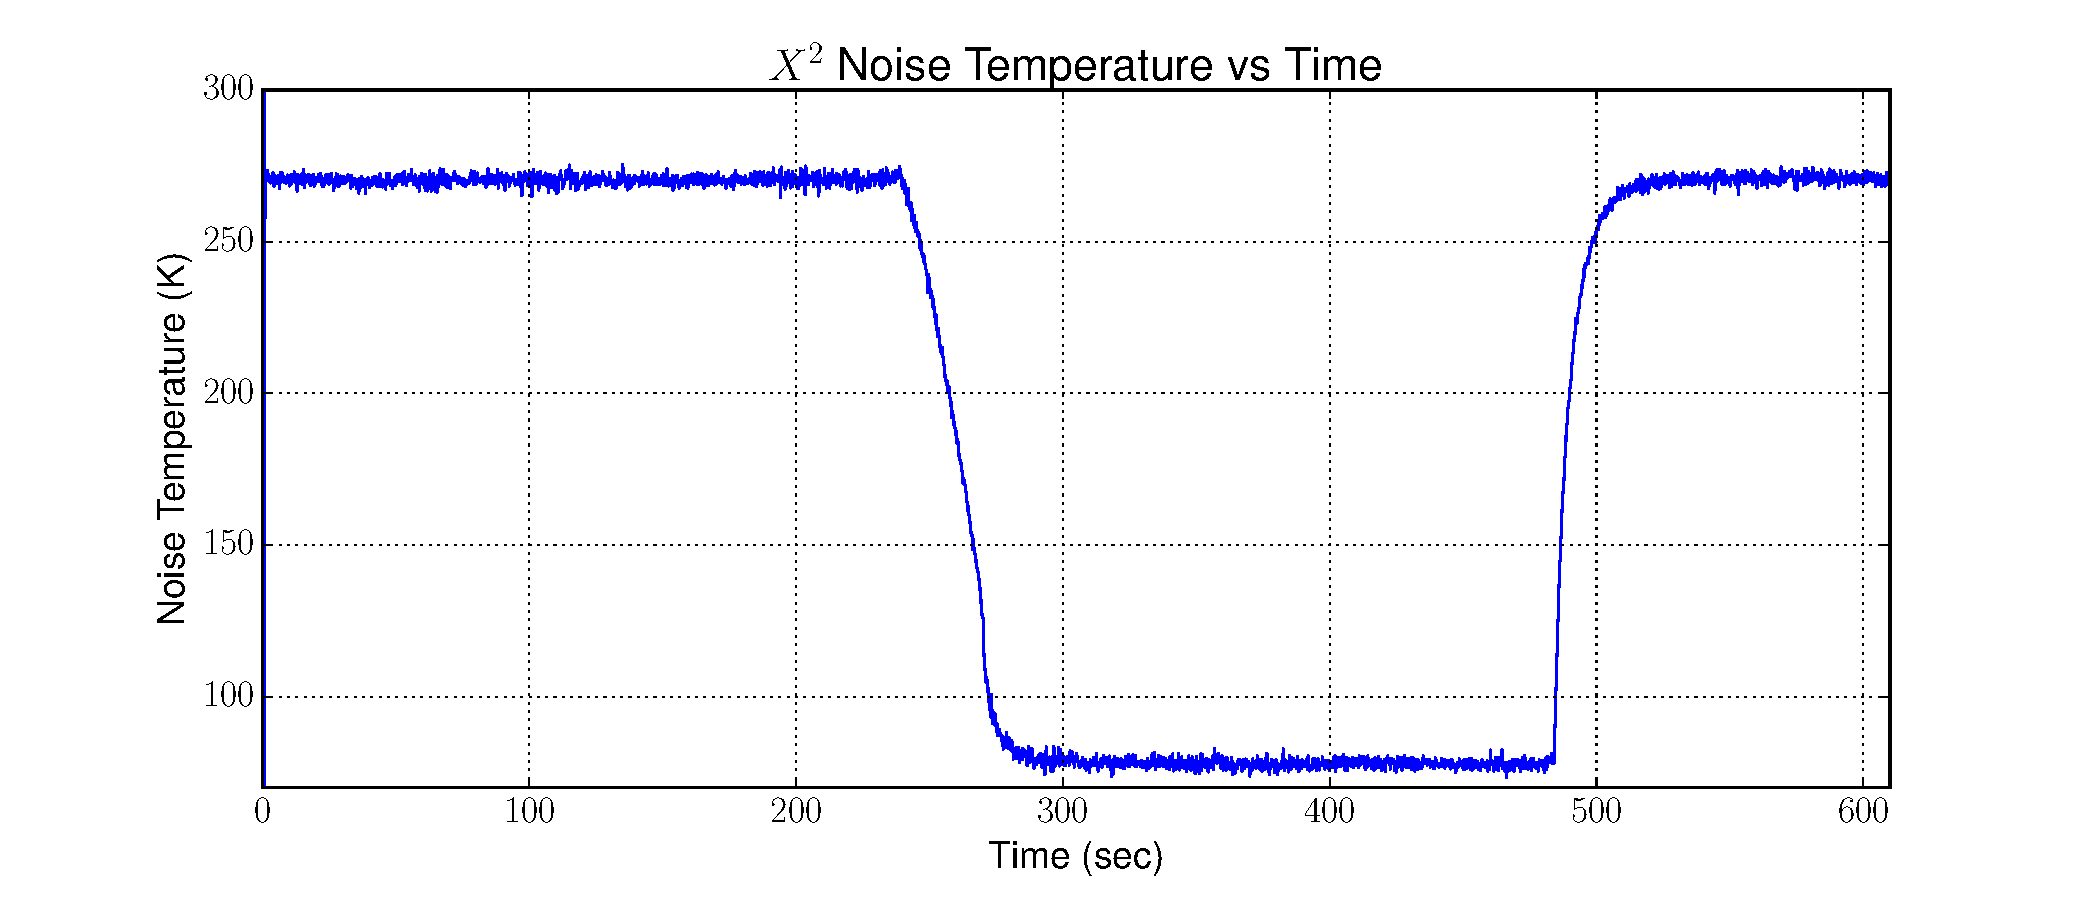
\includegraphics[width=\textwidth]{Experiments/Exp1/x2_calibrated.pdf}

\isucaption{Calibrated data from the square-law detector used in Experiment 1}
\label{X2_Calibrated}
\end{figure}

We now want to compare both the Software Defined Radio and the square-law to make sure that they match up.  Since both the SDR and the square-law are now calibrated to a noise temperature, we can easily graph both of the data and compare to see how well they match up.

\begin{figure}[h!tb] \centering

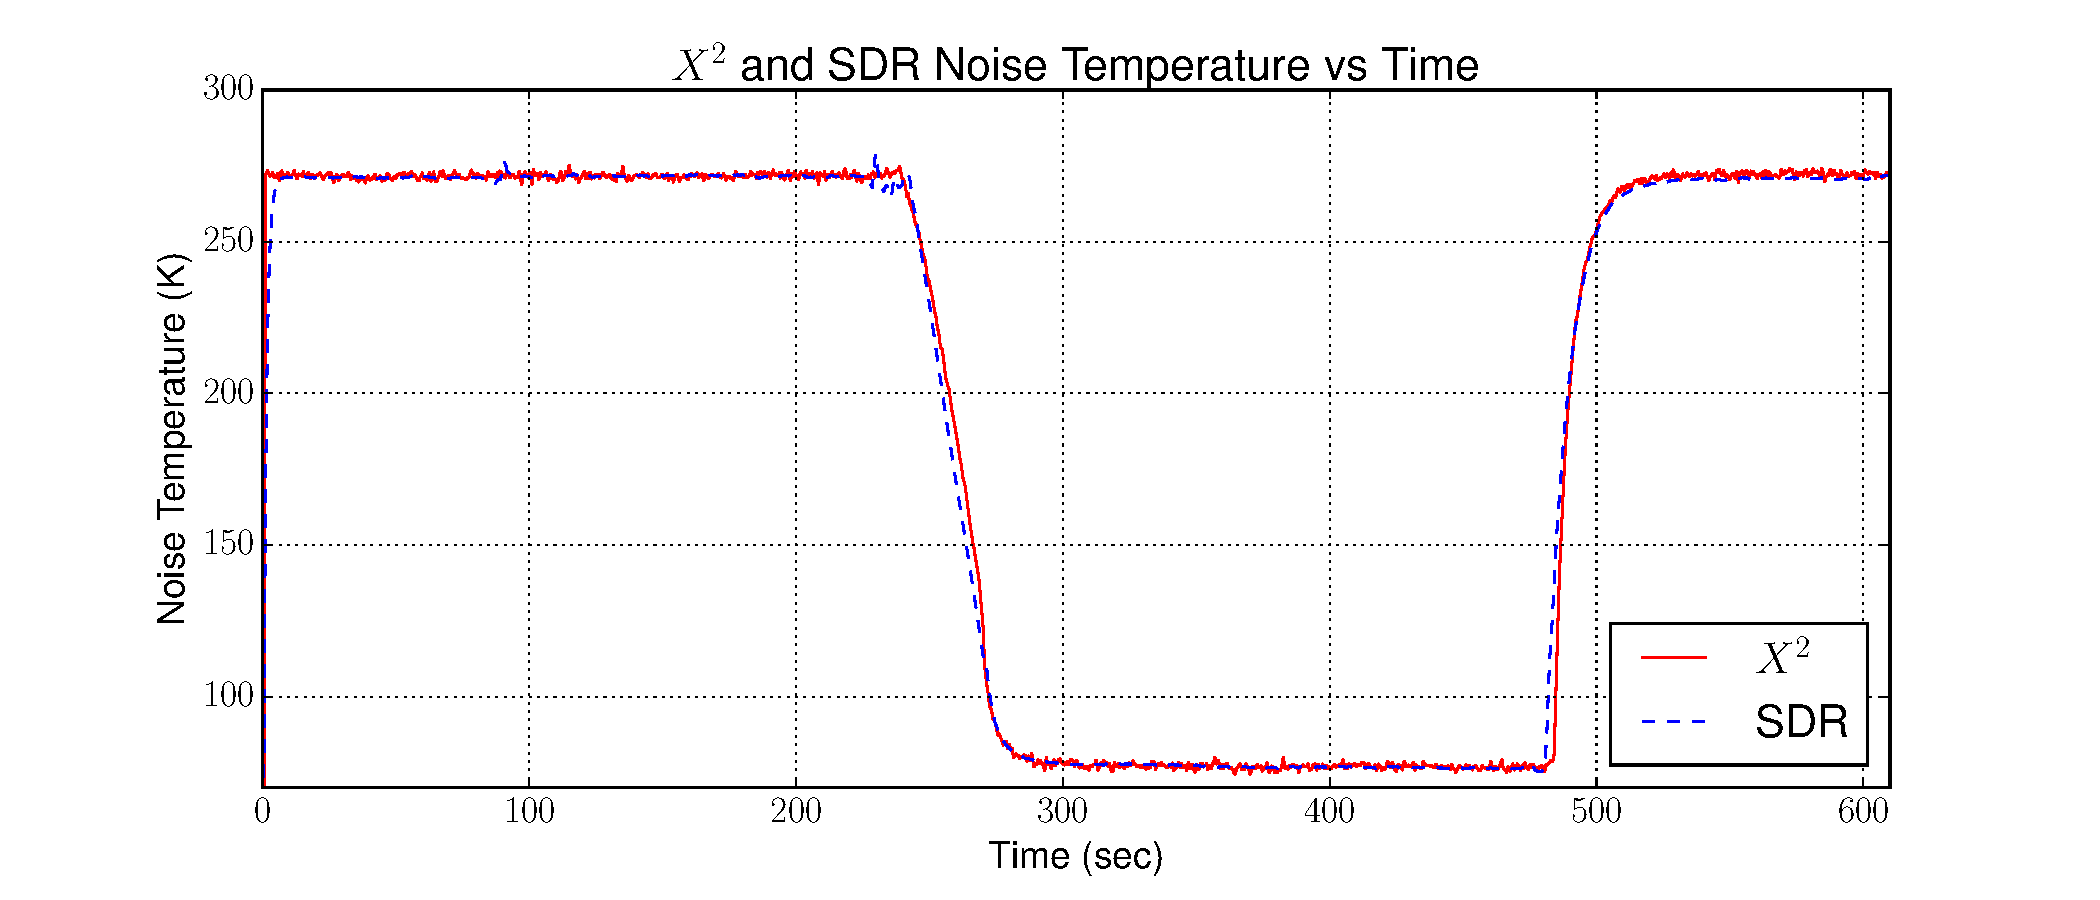
\includegraphics[width=\textwidth]{Experiments/Exp1/x2_SDR_Calibrated.pdf}

\isucaption{Figure showing both the SDR and square-law noise temperature data in Experiment 1}
\label{X2_SDR_Both}
\end{figure}

We can see in Figure \ref{X2_SDR_Both} that both the software defined radio and the square-law detector match up very nicely.  This shows that both the square-law detector and the software defined radio agree when properly calibrated.  This verifies that the software defined radio can indeed operate as a total power radiometer and the data we obtain from this setup agrees with an analog and more traditional radiometer.
\subsection{Application with Soil Moisture Readings}
A common application of radiometers is in the measurement of soil moisture.  All items naturally emit RF energy due to the random excitation by the electrons in the object.  The amount of noise that gets generated varies by temperature, but the amount that reaches the antenna varies by the amount of moisture in the soil.  If we can calibrate the radiometer to two known soil conditions, then we can measure the various levels of soil moisture in the soil.  At this time, we will simply look at the percentage of moisture in the soil, which will vary from zero percent or dry soil to one hundred percent or very wet soil.  The drier the soil, the more thermal noise we receive and the "warmer" the noise temperature.  Wet soil on the other hand attenuates the thermal noise and shows up as a "cooler" noise temperature.  

Using the Software Defined Radio, we can set up two methods to visually look at the noise temperature and thus the soil moisture percentage.  Since we do not have an antenna hooked up, we will simulate this by using two reference temperatures.  In this case the ice water bath and the LN2 that we just used and was shown earlier.  

A unique visual aid we can use with GNURadio is a waterfall display.  This display gives us information that includes frequency, amplitude and time.  It is referred to as a waterfall display due to the fact the display continually moves from top to bottom and looks like a waterfall.  Amplitude information is given by mapping the range of amplitudes to a color bar.  Frequency is given on the x-axis and time is on the y-axis.  Figure \ref{LN2_waterfall} shows a screen shot of the waterfall display in the GUI created in GNURadio Companion for this experiment.  This is the same program we have used but with the waterfall display now added.  The data for the waterfall is pulled directly from our source block or in our case the N200 software defined radio.

\begin{figure}[h!tb] \centering

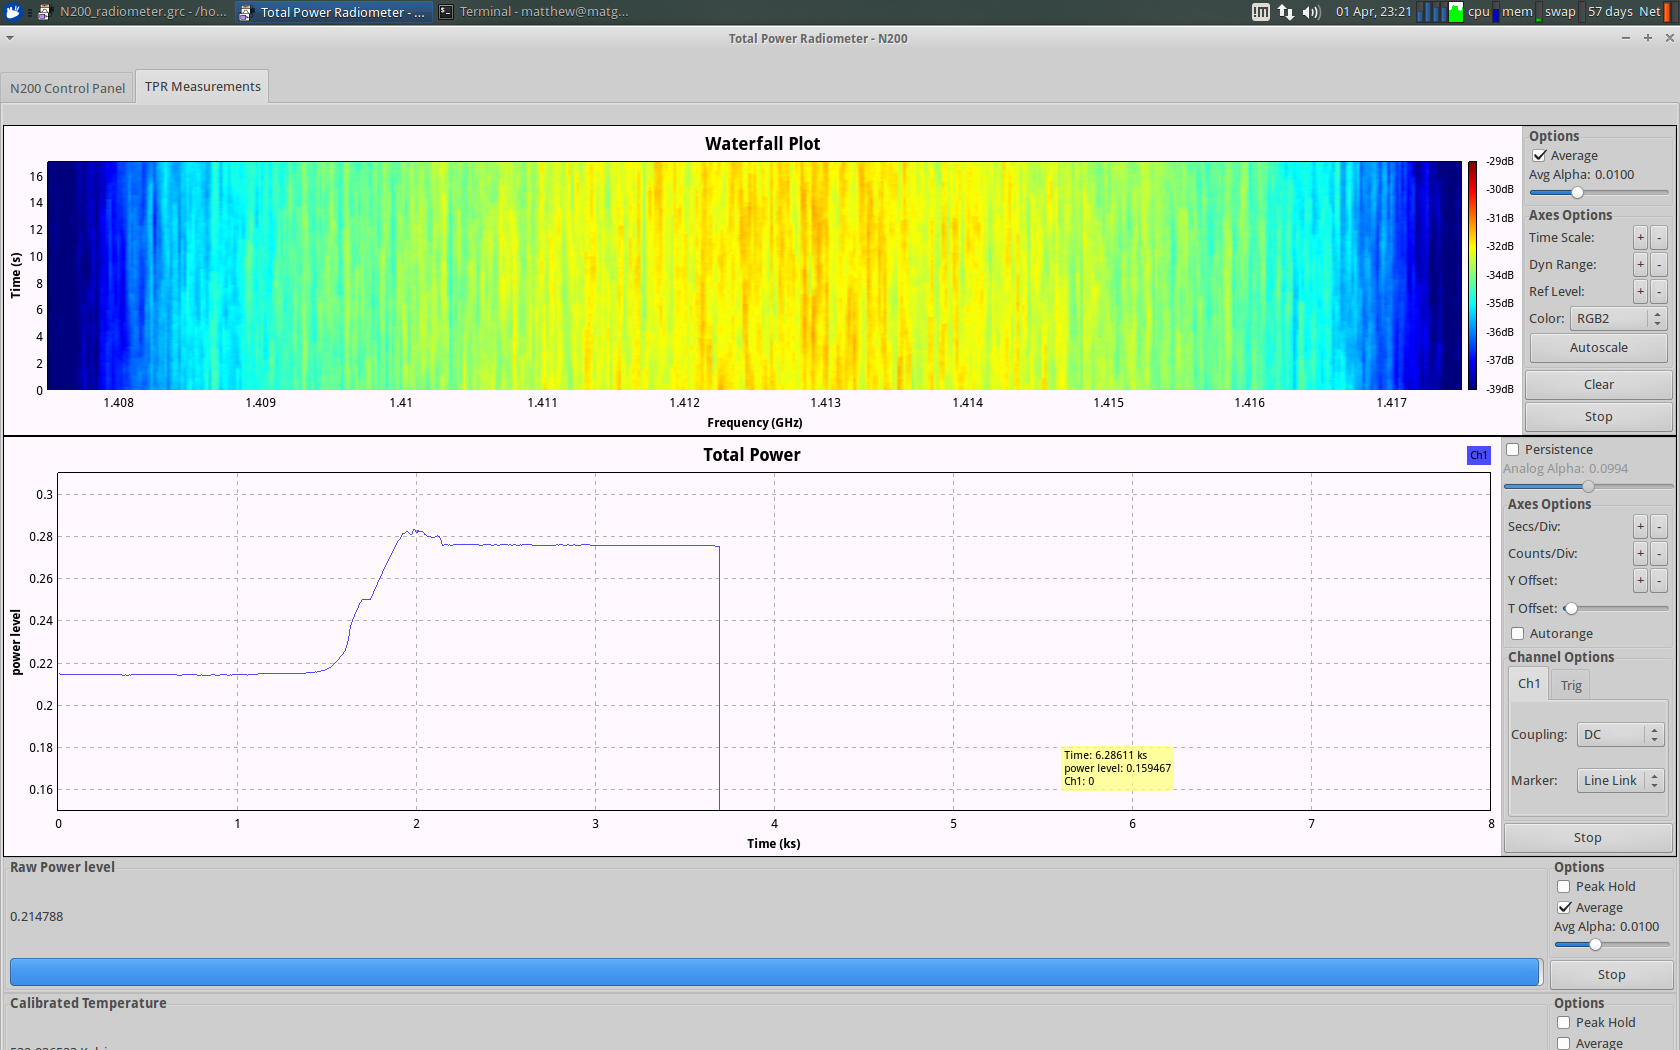
\includegraphics[width=\textwidth]{Experiments/Exp1/LN2_waterfall.png}

\isucaption{Screenshot of the waterfall display used in Experiment 1}
\label{LN2_waterfall}
\end{figure}

Let's take a look at two screen shots of the waterfall.  We will put them side by side so we can better compare the display when the thermal load is in the ice water bath and when the load is in LN2.

\begin{figure}[h!tb] \centering

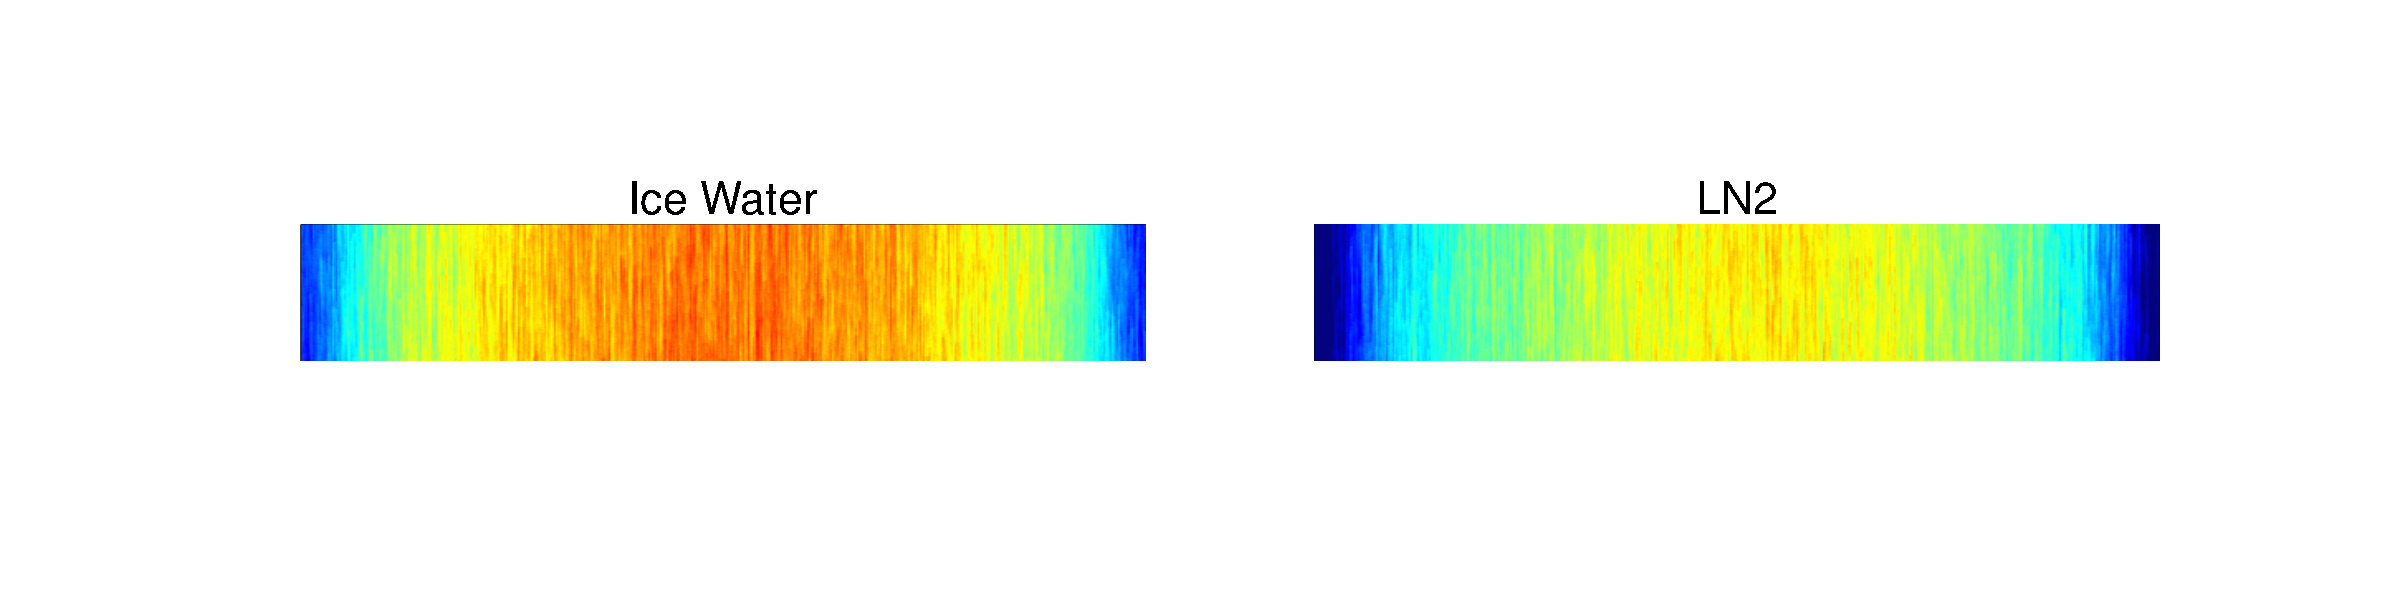
\includegraphics[width=\textwidth]{Experiments/Exp1/waterfall_side.pdf}

\isucaption{Side by side comparison of the waterfall display for Experiment 1}
\label{side_waterfall}
\end{figure}

In figure \ref{side_waterfall} we can see that the ice water screen shot appears warmer than the right side screen shot which appears cooler.  There is a limitation in GNURadio and the waterfall display that limits what the range for the power readings are.  The overall power that we see only changes by about 3 dB and our current range in the waterfall display is set to 10 dB.  If we could reduce the range, the color change would be even greater and more pronounced.  However, this does show that a change can be seen visually with color to indicate the noise temperature.  

If we assume that our LN2 is dry soil and that our ice water bath is wet soil, we can now interpolate the data to this scale and show the information we obtained in Experiment one as both a noise temperature and soil moisture.  Figure \ref{SDR_soil} shows the same data we looked at earlier but we have now added a scale to show soil moisture as a percentage.

\begin{figure}[h!tb] \centering

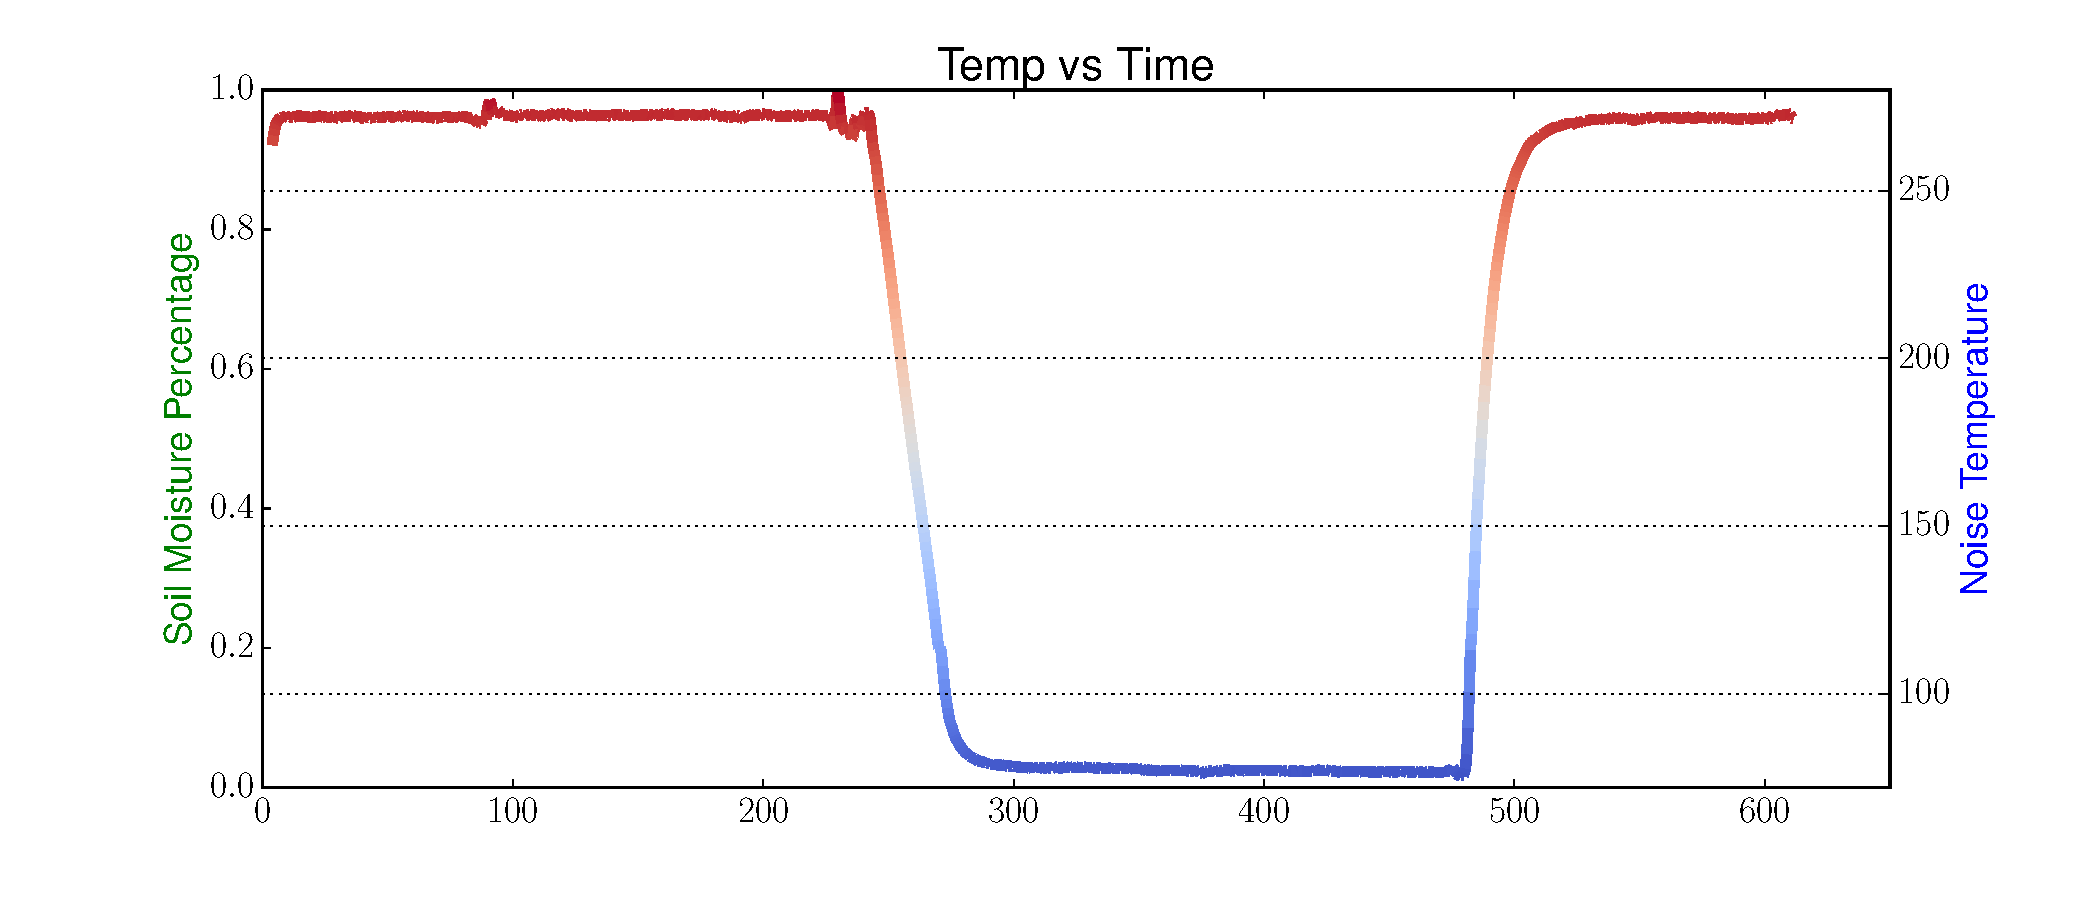
\includegraphics[width=\textwidth]{Experiments/Exp1/sdr_soilmoisture.pdf}
\isucaption{Plot of the noise temperature of Experiment 1 with soil moisture percentage}
\label{SDR_soil}
\end{figure}

While this demonstrates that we can collate our total power readings with a soil moisture percentage, we would use actual field tests to calibrate the radiometer.  In addition, we could also calibrate to soil moisture content instead of a percentage if desired.  Both methods have been done with traditional radiometers[\cite{Jonard}][\cite{Shi}.

\section{Data Analysis}





%Move this section once the stability section is established
To verify stability of the radiometer, we look to see how much change the radiometer records over a relatively long period of time.  To test this a matched load was submerged in a liquid nitrogen bath for an extended period of time, in this case for fifteen minutes.  The readings were then looked at to study the trend of the data.  The data is graphed in figure \ref{Stability}.

\begin{figure}[h!tb] \centering
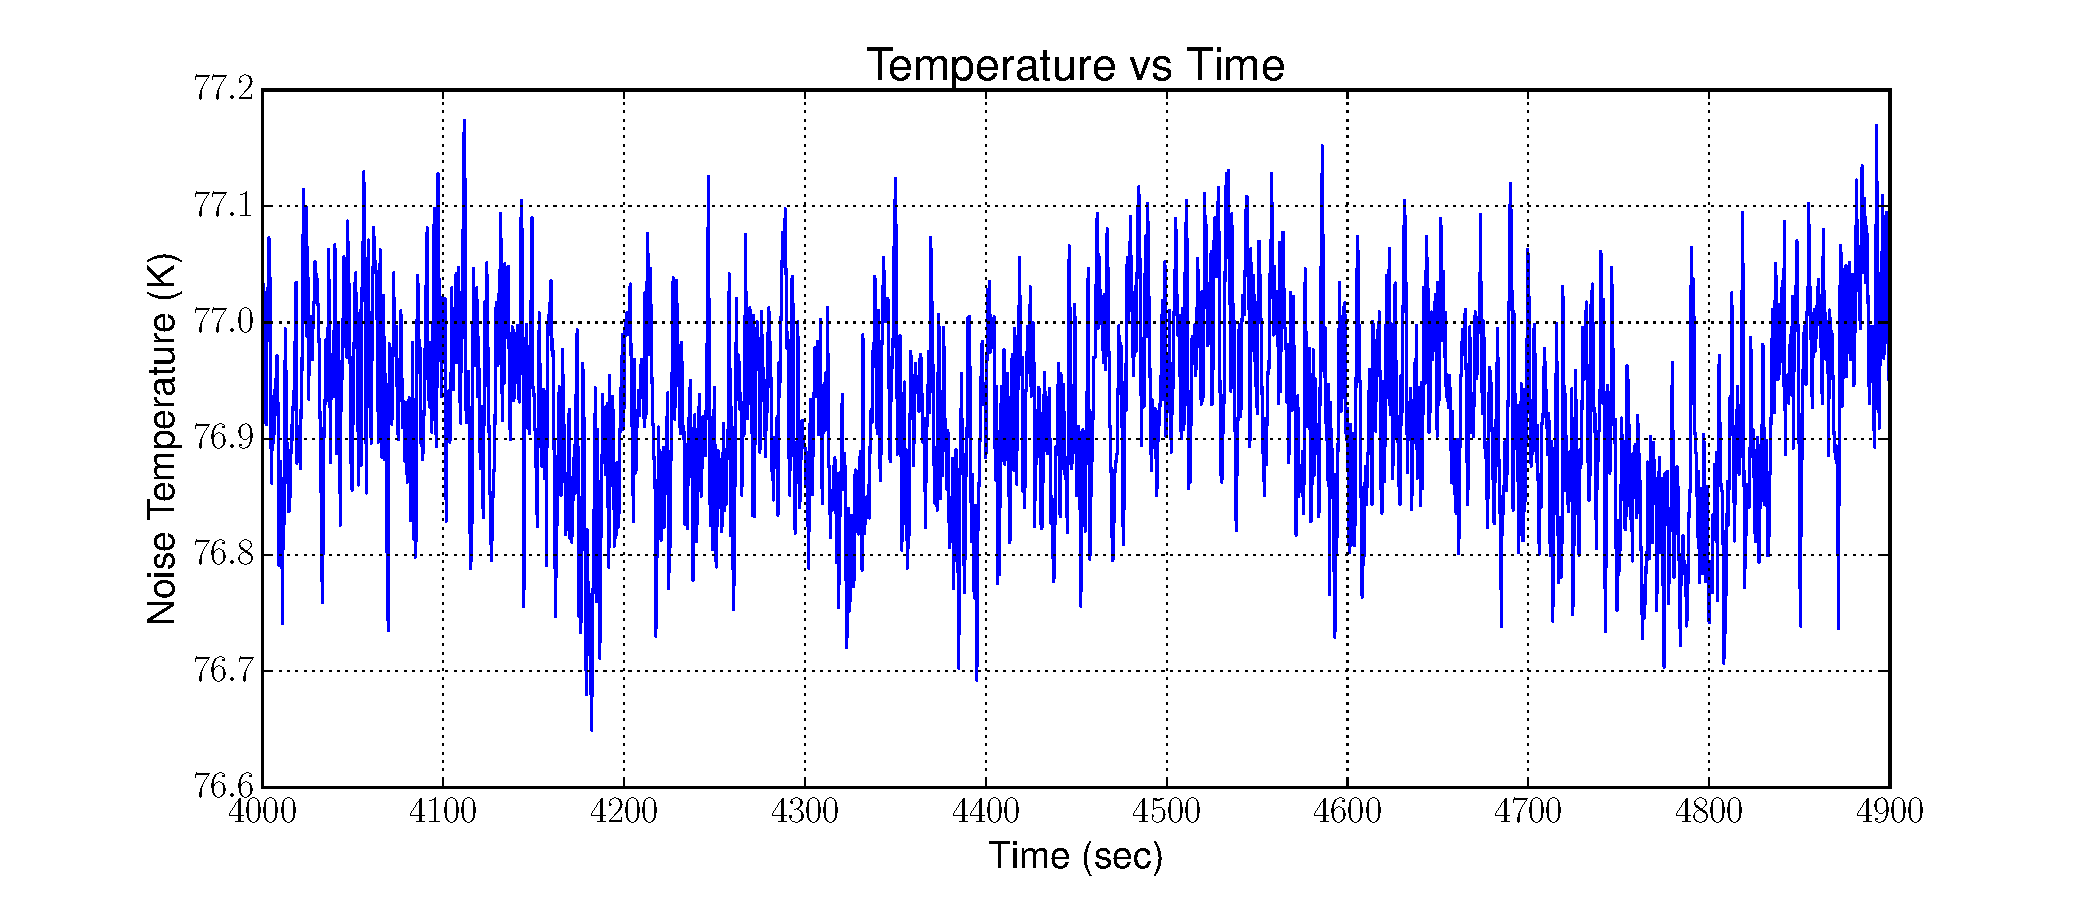
\includegraphics[width=\textwidth]{Experiments/Exp2/sdr_calibrated_zoom.pdf}
\isucaption{Graph of the calibrated total power over a period of fifteen minutes.}
\label{Stability}
\end{figure}

\begin{figure}[h!tb] \centering
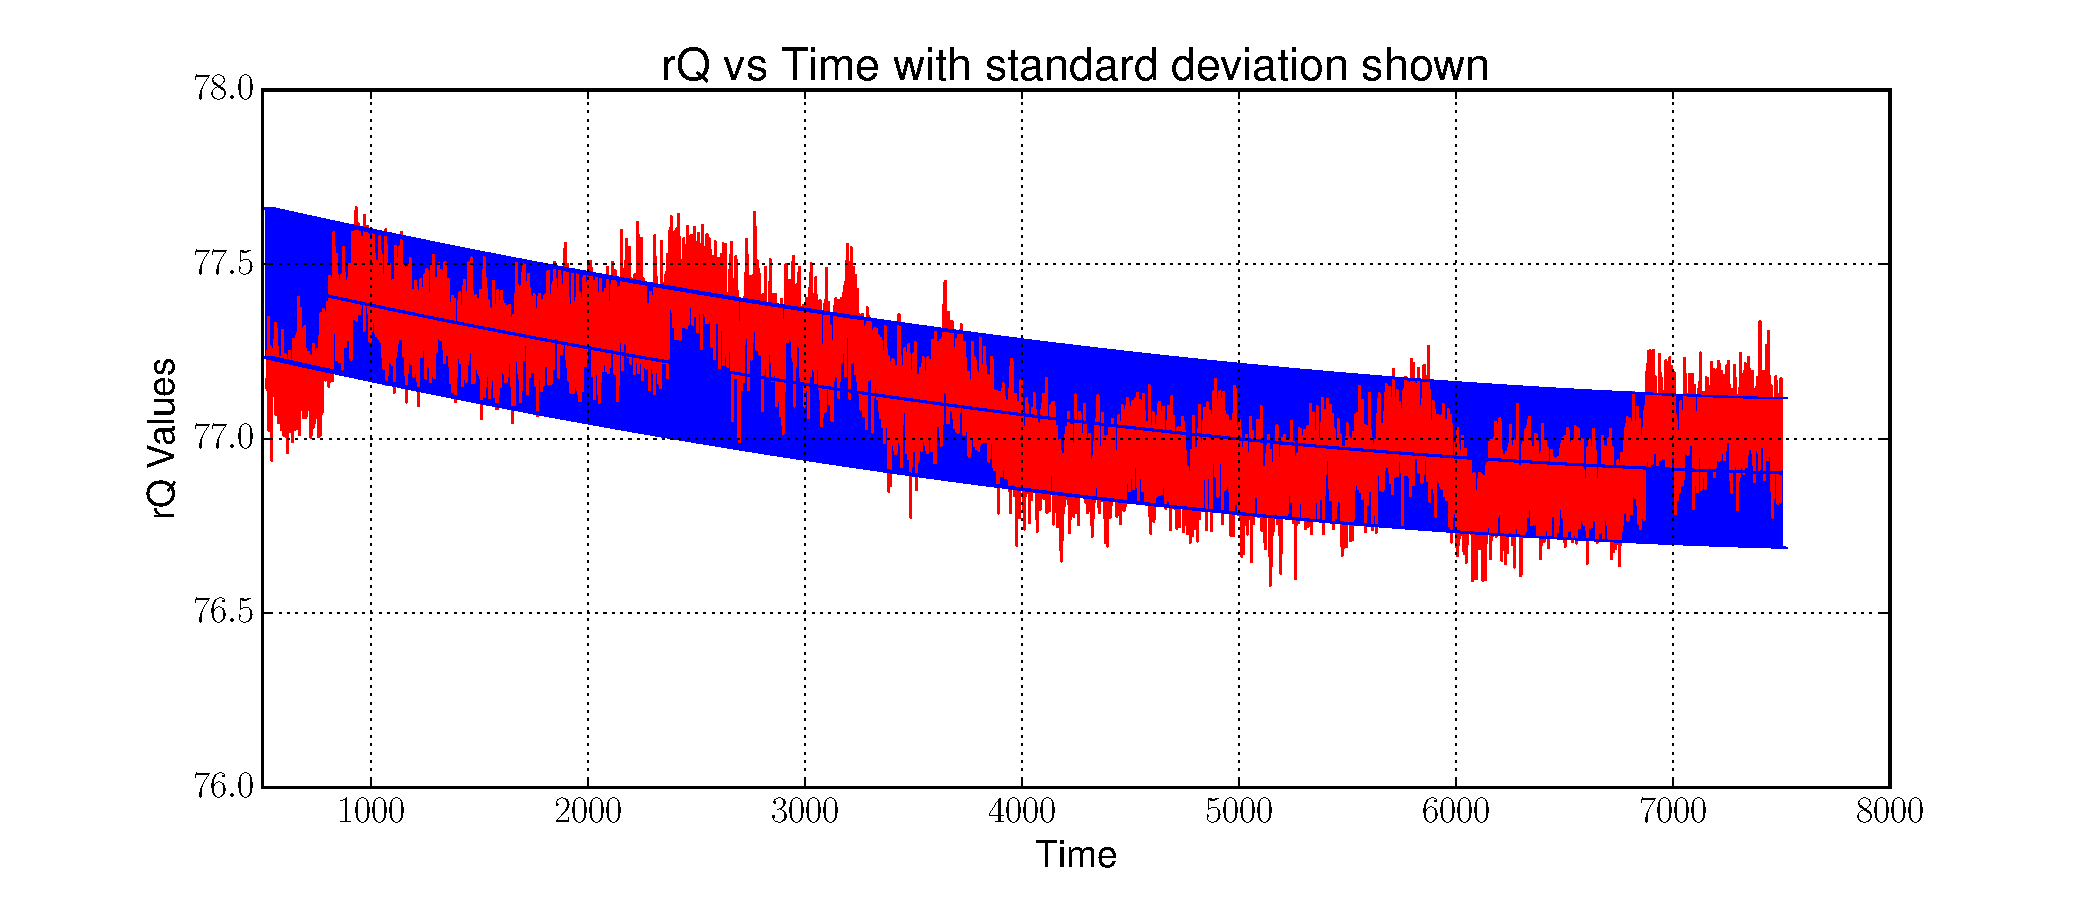
\includegraphics[width=\textwidth]{Experiments/Exp2/calib_vstime_stddev.pdf}
\isucaption{Graph of the calibrated total power with the standard deviation plotted.}
\label{Stability_calib}
\end{figure}

As it can be seen in figure \ref{Stability}, the amount of change over a period of one hour is quite small.  The standard deviation for this sample is 0.09 kelvin.  The $NE\Delta T$ calculated using 10 MHz for the bandwidth, an integration time of 2 seconds and with our sample at 77 Kelvin is calculated to be 0.10 Kelvin with a system temperature of 350 Kelvin.  Therefore, our system is behaving as we expect it to for this stability test.

Figure \ref{Stability_calib} shows a graph of the total readings but with the standard deviation now plotted.  This shows that the system is stable and is operating as expected within our expected $NE\Delta T$.

%---------------------------------------------------------------


Once the experimental data was obtained the next step is to analyze the data and format the data so that it is easy to read and comprehend.  The total power readings and the raw I/Q data generated from GNURadio is stored as a binary file stored in little-endian format.  Total power data is stored as a float values and I/Q data is stored as complex values.  Data from the square-law detector is stored as a comma delimited ASCII file.

Matlab is one tool we can use to process the information that is stored by GNURadio.  Appendix A contains the Matlab source that will read the total power file generated by GNURadio.  It then calculates information such as the NE$\Delta$T and the calibration points based on the user input.  We can also use Matalb to graph this information as well.

While Matlab is one tool, other tools can be used.  Python for example is also capable of reading in these files and when paired with NumPy and SciPy can be used to perform analysis on the data as well [\cite{Uengtrakul}].  In addition, the open source mathematical program Octave should also be able to read and work with these files.  For this thesis both Matlab and Python was used to provide analysis on the data.  

Most of the graphs generated in this thesis was generated using iPython notebooks.  IPython notebooks uses Python but allows it to be executed in a web browser either locally or on a server.  Using iPython notebooks however also allows us to add additional information using Markdown and basic HTML.  This allowed the author to paint a complete picture of the experimental results illustrating pictures of the setup and the code and steps used to analyze the data.  You can find these notebooks on the author's Github site and can use NBViewer to view them.  An example link is \href{http://nbviewer.ipython.org/github/matgyver/Radiometer-SDR-Thesis/blob/master/Experiments/Exp1/radiometer_experiment_1.ipynb}.

{\begin{figure}[h!tb] 
\centering
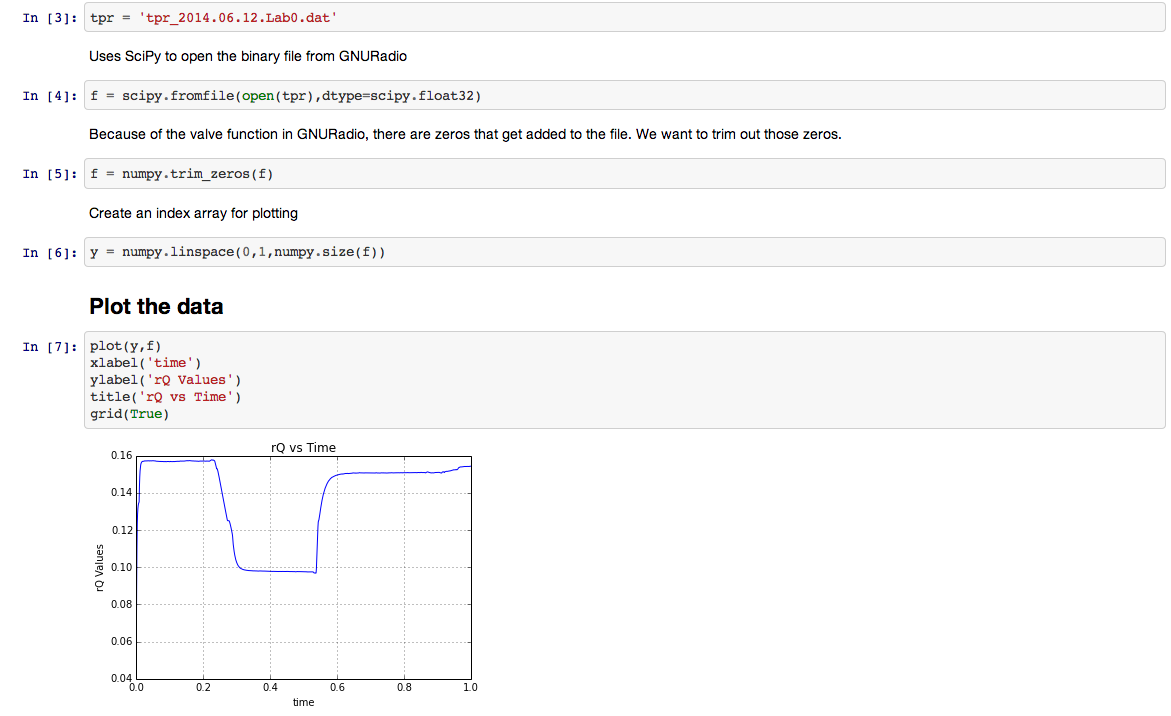
\includegraphics[width=17cm]{Images/python_gnuradio.png}
\isucaption{A screenshot showing the iPython notebook code and related graphs generated for parsing GNURadio data}
\label{matlab_display}
\end{figure}

\section{Benefits to Software Defined Radio Radiometer}
A study was conducted on what benefits a software defined radio radiometer would have over a more traditional radiometer.  This was focused on looking at three main areas; cost, weight and size, and the value a SDR radiometer can add over traditional radiometers.

\subsection{Cost Benefits}
Software defined radios have become more commonplace in recent years and this has generated a number of Commercial Off The Shelf (COTS) solutions.  A COTS solution is often a lower cost solution due to the mass manufacturing that takes place.  This has driven the cost of many SDRs to under one thousand dollars while still having excellent performance characteristics.  The N200 SDR purchased for this research cost fifteen hundred dollars and the daughter-board cost one hundred and fifty dollars approximately.  Other software defined radios however have come out on the market since then.  Ettus for example has some that are below one thousand dollars and the author has also obtained the HackRF One SDR that now sells for three hundred dollars.  The main difference with the different software defined radios on the market is with both the resolution, or how many bits the ADC is, and the bandwidth they are able to handle.

\begin{table}[h!tb] \centering
\isucaption{Cost Analysis}
\label{cost_table}
% Use: \begin{tabular{|lcc|} to put table in a box
\begin{tabular}{lcc} \hline
\textbf{Device} & \textbf{Quantity} & \textbf{Cost} \\ \hline
\textbf{SDR Solution}& & \\ \hline
N200 SDR & 1 & \$1515 \\
LNA at \$60 ea. & 3 & \$180 \\
DBSRX2 Daughter-board & 1 & \$152 \\
GNURadio & 1 & \$0 \\ \hline
Total & & \$1847 \\ \hline
\textbf{ISU Radiometer} \\ \hline
LNA, FPGA, ADC, Microcontroller and power supplies & 1 & \$10,000\tablefootnote{Purchase price in 2005} \\ \hline
\textbf{Commercial Off the Shelf Unit}\\ \hline
Spectracyber 1420 MHz Hydrogen Line Spectrometer & 1 & \$2,650 \\ \hline

\end{tabular}
\end{table}

As see in table \ref{cost_table}, even the higher cost Ettus research equipment is a lower cost option than the custom built ISU radiometer purchased from University of Michigan and even a comparable off the shelf radiometer.  It should be noted that the radiometer from the University of Michigan is also a dual polarization radiometer so there are two RF front ends and two ADCs that feed into a FPGA board.  It would be quite easy to add dual polarization to the Ettus N200 SDR as it does support two daughter-boards.  This would increase the cost to \$2,179 for the additional LNAs and daughter-board.

The largest cost benefit is that key components that you find in a radiometer, the filters and square-law detector can now be all done in software instead of needed additional equipment.  The system is also much more frequency agile, which means it can work on a broader range of frequencies than most traditional radiometers with very little change in hardware and in some cases may require no change in hardware.  Some of this does depend on the SDR hardware however.  The Ettus N200 for example uses daughter-boards to provide the RF interface.  While these boards provide a high quality in the RF signal, it does come at a cost and are usually designed for certain bands of frequencies.  Other low cost SDRs however are also very wide range in the frequencies they will work in.  The HackRF for example works from 10 MHz to 6 GHz, but does so at the cost of lower resolution, less gain in its front end and a lower bandwidth that it can handle.

\subsection{Weight and component size benefits}

A typical radiometer has many components that are involved in the design of the radiometer.  This includes filters, LNAs and the power detection or square-law detector used.  These components add both weight, size and costs to the radiometer.  A software defined radio however digitizes the signal and we are able to replace the filters and square-law detector with their software equivalent.  While a software defined radio does add both the ADC and usually a FPGA to do the processing on the signal, advances in semiconductor technology has continued to shrink these components.  These components are also lighter than the filters often used in radiometers.

\begin{table}[h!tb] \centering
\isucaption{Weight Analysis}
\label{weight_table}
% Use: \begin{tabular{|lcc|} to put table in a box
\begin{tabular}{lc} \hline
\textbf{Device} & \textbf{Mass} \\ \hline
\textbf{SDR Solution} & \\ \hline
N200 SDR & 1.2 kg \\
LNA at .03 kg ea & .09 kg \\
DBSRX2 Daughter-board & .1 kg \\ \hline
Total & 1.39 kg \\ \hline
\textbf{ISU Radiometer} \\ \hline
LNA, FPGA, ADC, Microcontroller and power supplies & 22.7 kg \\ \hline
\textbf{Commercial Off the Shelf Unit}\\ \hline
Spectracyber 1420 MHz Hydrogen Line Spectrometer & 6 kg\tablefootnote{Estimated, no data available} \\ \hline

\end{tabular}
\end{table}

Size is another benefit as since semiconductor technology has continued to shrink components.  Again, since items like the filters and square-law detector are removed and done in software this helps to reduce the overall size.  

\subsection{Value added benefits}

A software defined radio radiometer adds additional value for two reasons.  One, it is able to work with both frequency and magnitude where most radiometers do not.  This allows for additional analysis on the signal and can help identify issues such as an interfering signal that was demonstrated in this thesis.  

Second, we are able to have an agile system that is able to adapt to changing conditions with very little or no change to hardware.  Different types of radiometers can be implemented such as a Dicke radiometer, dual polarization radiometer or a radiometer that can perform Stokes parameters.  In addition, since we have both frequency and power information we can create a system that is able to adapt to changing conditions such as dealing with an interfering signal.  

\section{Disadvantages of a SDR Radiometer}
Although we have outlined a number of advantages of using a COTS SDR Radiometer and how a SDR can add additional value to the radiometer system, there are some disadvantages to a SDR Radiometer.

\subsection{Power Consumption}
One of the largest drawbacks to a SDR radiometer can be in the power consumption of the SDR.  With the move to perform functions such as power detection and filtering we now require additional computational power to perform these tasks.  With those computational cycles additional power is now required.  The use of FPGAs and SoC however can help to minimize these power concerns as they are more efficient than using a full scale x86 based processor and on board computer system.  

Power and CPU requirements also increase as we add additional functionality such as filtering an offending signal.  While these additions may not require additional hardware, it can require additional processor or computational requirements.  This will cause additional strain on the processor and also in the memory requirements for the SDR as well.

\subsection{Bandwidth constraints}
While SDR technology has advanced, bandwidth is still a constraint that affects SDRs and in turn a SDR Radiometer.  Bandwidth plays a critical role in the radiometer's sensitivity as explained in this thesis, therefore the fact that many SDRs are limited in bandwidth does create a disadvantage.  In many cases this bottleneck takes place in both the transport and processing of large bandwidth systems.  This also relates to the power consumption disadvantage since larger bandwidth also means requiring additional computational cycles as well.  

In contrast, a square-law detector usually has a very large bandwidth, as much as one gigahertz, and is why we usually need to filter to the frequency band of interest.  

\section{Results Summary}

%----------------------------------------------------------
% End of Chapter 6.  Anything below this is extra information

%The data collected was then graphed using Excel.  The graph shown in \ref{adl5902_linear} shows that the ADL5902 has a linear output and matches the expected value based on the input.  

%\begin{figure}[h!tb] \centering
%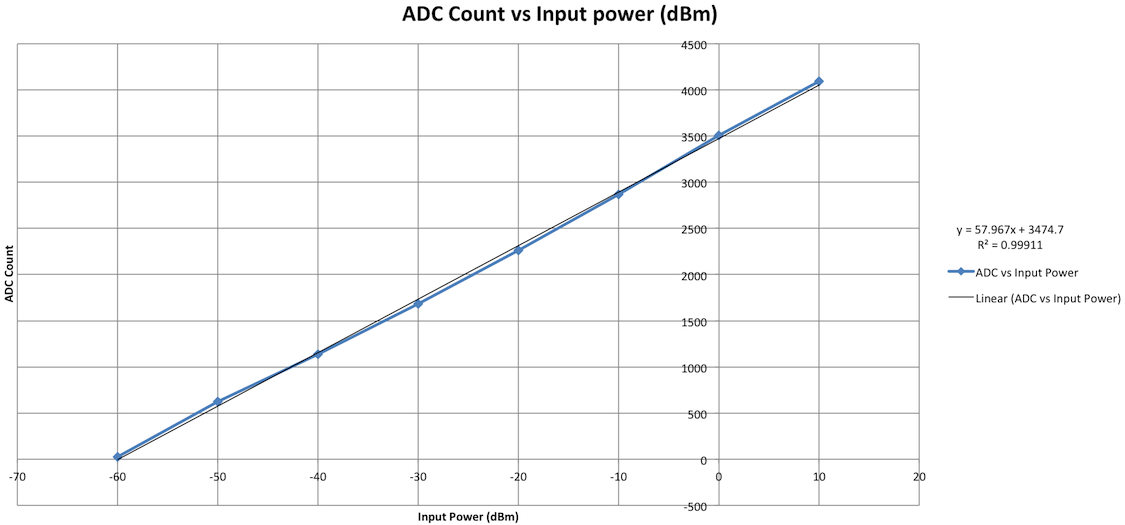
\includegraphics[width=\textwidth]{Images/Linearsquarelaw}
%\isucaption{Graph showing the linearity of the ADL5902}
%\label{adl5902_linear}
%\end{figure}

%Once it was confirmed the ADL5902 does in fact have a linear response, we then looked at ways to work with the ADL5902.  The graph above was generated using Analog Devices program that talked to the Blackfin processor on the daughter-board.  However, the information for talking to the Blackfin is proprietary.  Therefore, the daughter-board was removed for future tests and instead we used the USB-6009 data acquisition board to read the raw analog voltages from the ADL5902.  This information was then stored later for additional analysis.  


% Appendix1 file from standard thesis template
\appendixtitle
\appendix
\chapter{Source code}

The following is the source code to several programs that make the radiometer possible.  The first is the Python code used with the Ettus N200 software defined radio.  This python code should work on any platform that has the GNURadio libraries installed and also the USRP drivers for communicating with the N200.  This code can also be easily modified to communicate with any SDR that GNURadio can communicate with.  This code was generated using GNURadio Companion.  

The second code is the Matlab script that can be used to parse the output from GNURadio.  This code will plot the total power output as well as perform some other functions such as a NE$\delta$T calculation and also allows for calibration points to be entered as well.  This code can be used as a foundation for other programs.  

The third code supplied is Python code that can be used to read the data generated and plot it.  In many ways it mimics the functions of the Matlab script buy uses Python, NumPy and SciPy to perform the mathematical functions.  This may be a better option for those that wish to look at the data but do not have access to Matlab since Python is free to download.

Finally, this code has been included in this thesis as a point of reference.  It may be out of date and some other pieces of code was also used for the experimentation used in this thesis.  Copies of this thesis source \LaTeX code, and any other code used can be found on the author's GitHub repository, \url{https://github.com/matgyver/Radiometer-SDR-Thesis}.


\section*{Python code for total power radiometer}
\lstset{
  language=Python,
  showstringspaces=false,
  formfeed=\newpage,
  tabsize=4,
  commentstyle=\itshape,
  basicstyle=\ttfamily,
  breaklines=true,
  morekeywords={models, lambda, forms}
}

\newcommand{\code}[2]{
  \hrulefill
  \subsection*{#1}
  \lstinputlisting{#2}
  \vspace{2em}
}

\code{Total Power Radiometer}{Code/N200_TPR.py}
\newpage

\section*{Matlab code for reading and displaying data from GNURadio}
\lstset{
  language=Matlab,
  showstringspaces=false,
  formfeed=\newpage,
  tabsize=4,
  commentstyle=\itshape,
  basicstyle=\ttfamily,
  morekeywords={models, lambda, forms}
}

\newcommand{\matlabcode}[2]{
  \hrulefill
  \subsection*{#1}
  \lstinputlisting{#2}
  \vspace{2em}
}

\matlabcode{GNURadio Parsing Code}{Code/gnuradio_parse.m}
\newpage

\section*{Python code for analyzing data}
\lstset{
  language=Python,
  showstringspaces=false,
  formfeed=\newpage,
  tabsize=4,
  commentstyle=\itshape,
  basicstyle=\ttfamily,
  morekeywords={models, lambda, forms}
}

\newcommand{\pythoncode}[2]{
  \hrulefill
  \subsection*{#1}
  \lstinputlisting{#2}
  \vspace{2em}
}

\pythoncode{Total Power Radiometer}{Code/iPython/Radiometer_Parse.py}
\newpage
% An example second appendix from the example thesis thesis.tex.
\chapter{EE 518 Test Results}

\section*{E E 518 Lab Tests}

Further testing of the square-law detector was performed by using the radiometer in a real world event.  This test was exercised in conjunction with the Microwave Remote Sensing class (E E 518) under Dr. Brian Hornbuckle.  In the Spring of 2012 the radiometer was moved to the roof of agronomy and the EE 518 students conducted a number of tests using the N200 software defined radio to collect the data.


{\begin{figure}[h!tb] 
\centering
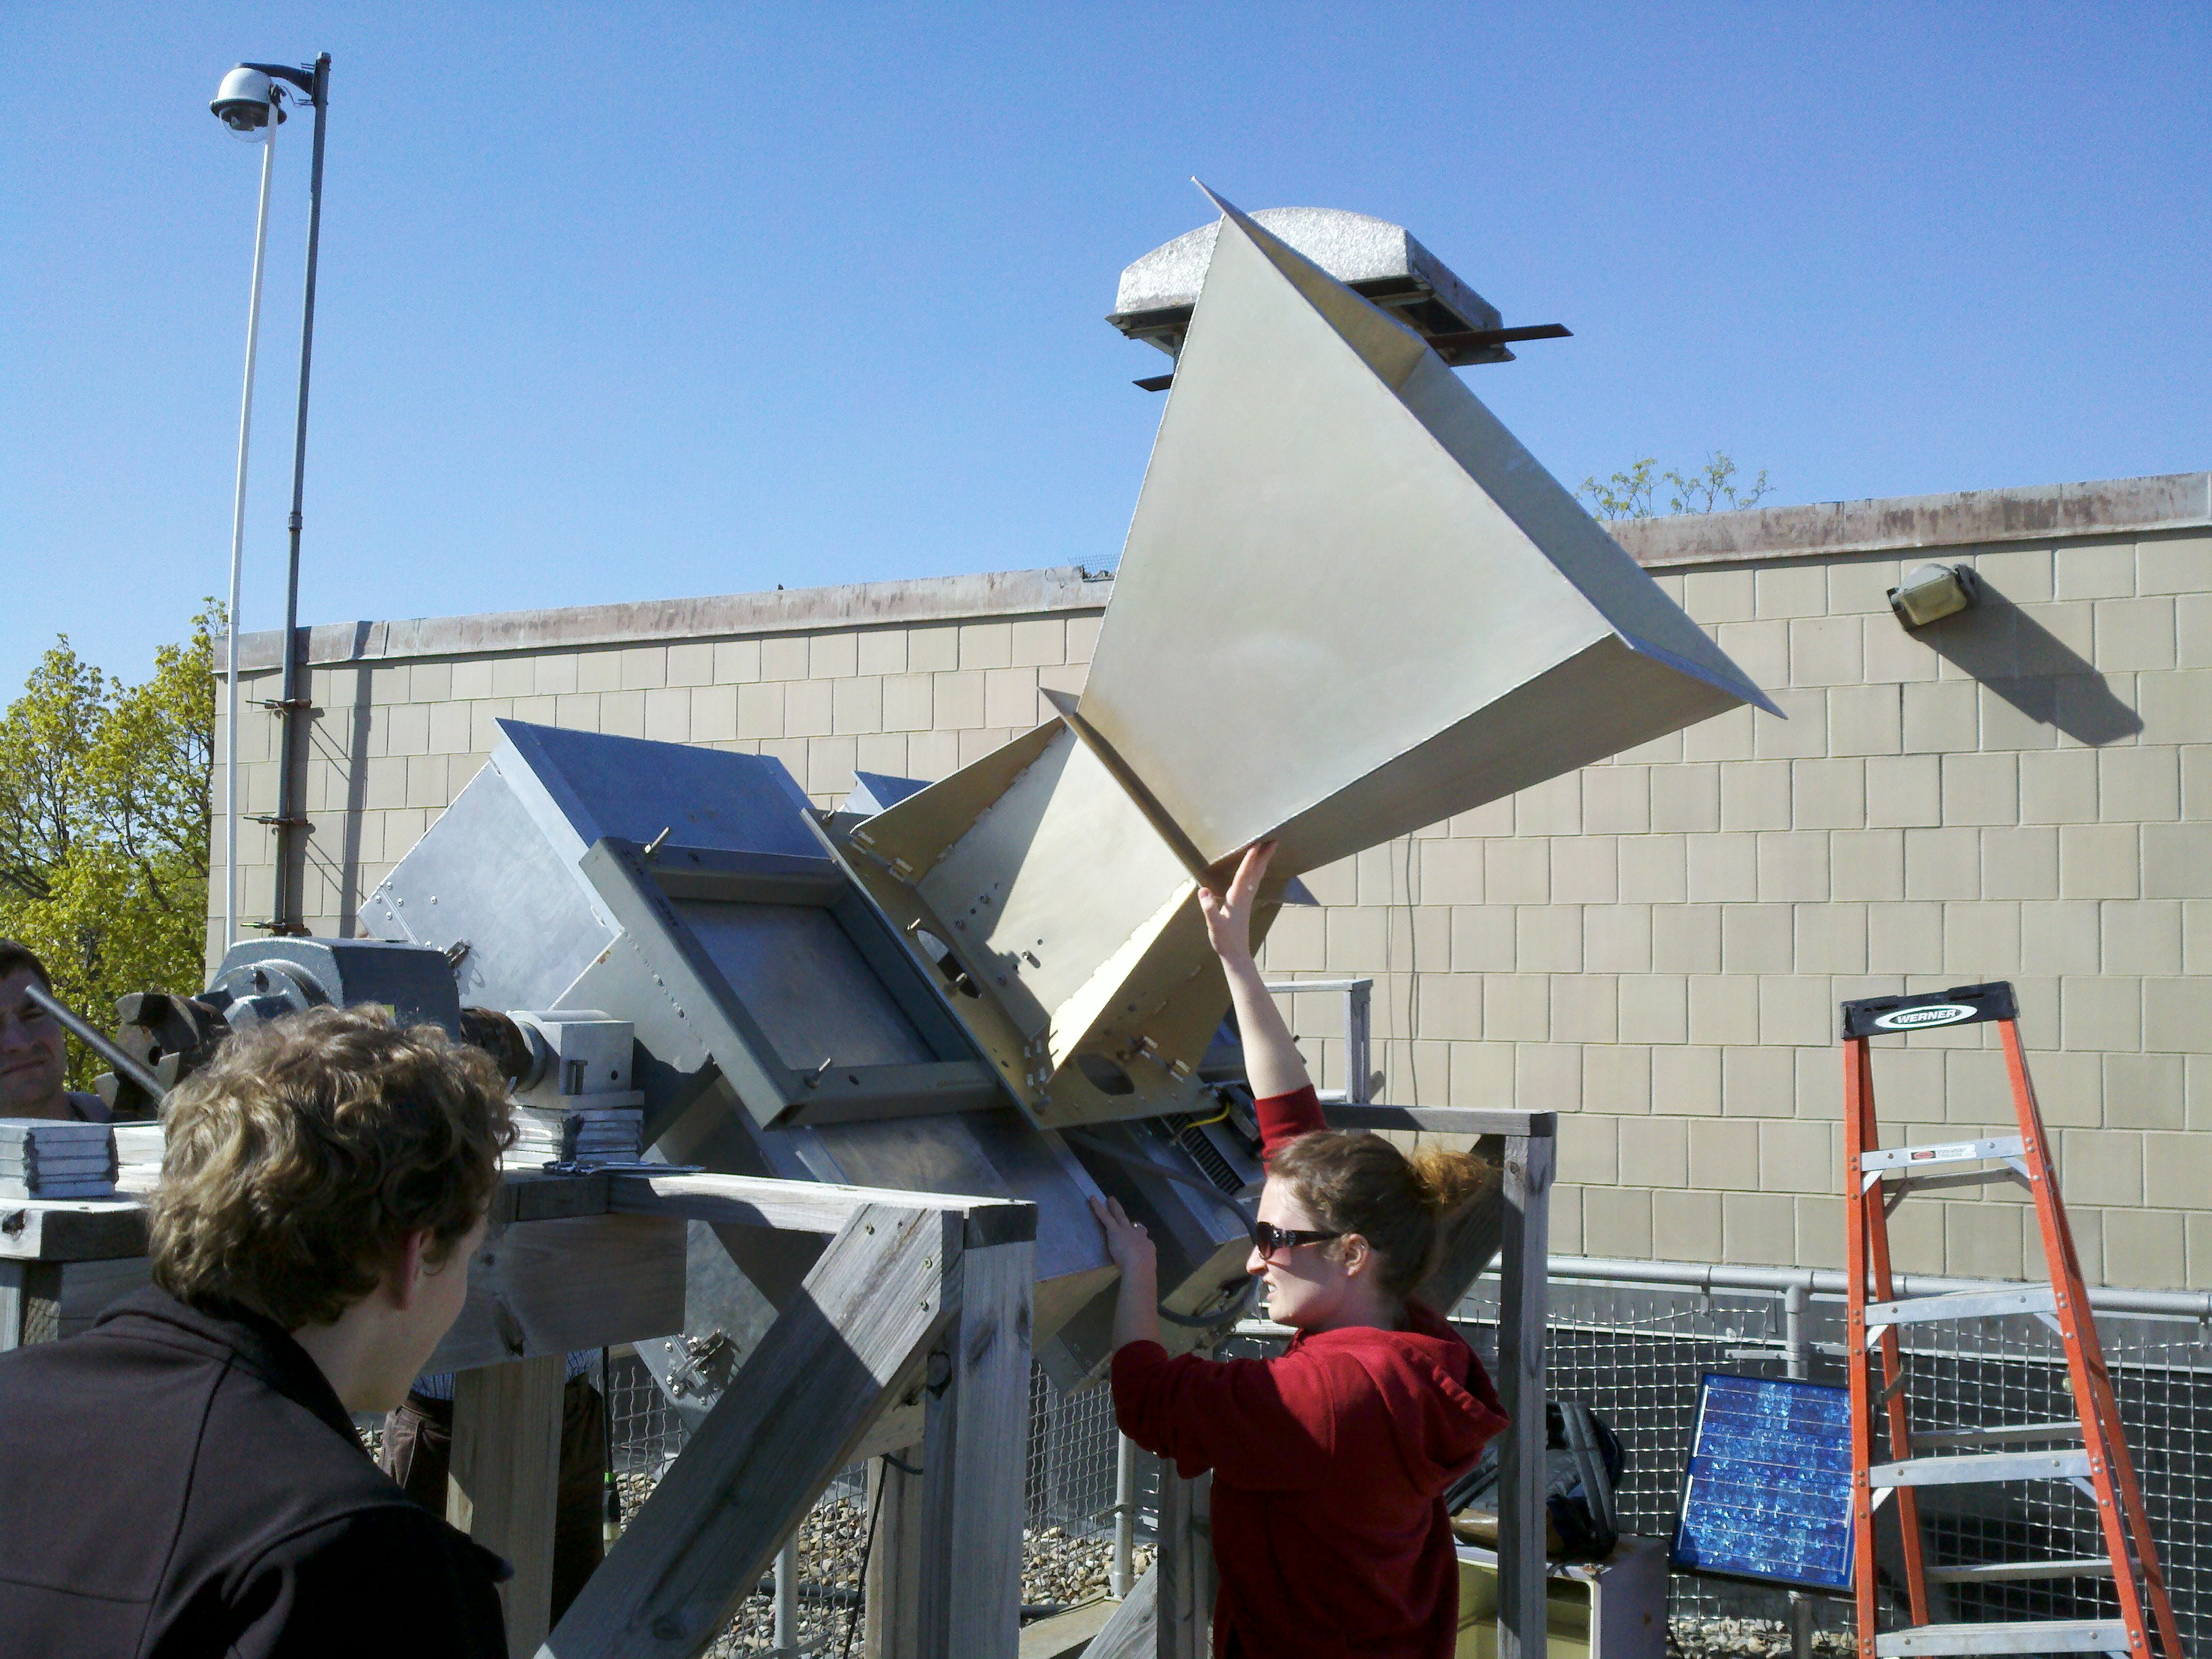
\includegraphics[width=\textwidth]{Images/radiometer_roof.jpg}
\isucaption{Students rotating the radiometer for an experiment on Agronomy Hall}
\label{radiometer_roof}
\end{figure}
}

The E E 518 test however showed that there were additional problems with the radiometer.  While the test showed that the SDR could in fact read data, the data was skewed.  It was later found out that the radiometer was generating an interfering signal that caused the power readings to be elevated.  It was also found that the interfering signal was also flucatating and seemed to correspond somewhat to the physical position of the radiometer.  This was found as a result of having the SDR record the raw I/Q values and then was analyzed later.  Through this analysis, we found that a strong harmonic was developed and caused a spike in signal being recorded.  Although the exact reason for this has not been found, the problem has been isolated to something in the RF Front End of the ISU radiometer. 

In the Spring of 2014 the E E 518 class ran another experiment, but this time a different one.  This experiment mimicked the experiments that the author ran to calibrate and test the radiometer.  This allowed an outside source to validate the results that I was getting with running the radiometer.  Like my tests, the students submerged a matched load into liquid nitrogen and then in boiling water.  The liquid nitrogen was assumed to be at 77 K and the boiling water was measured to be at 99 C or 372 K.  The students were then given a mystery sample in which they had to determine the temperature of a water sample.  Since the students had to points, they could find the calibration line and determine the temperature.  The experiment was run twice as we expected the radiometer may have drifted between measurements.  

\subsection{Test setup}
For the E E 518 class, the setup was similar to experiments that was run to test the results in this thesis.  For the E E 518 however the students only used the N200 SDR for recording the total power readings.  The ISU Radiometer was used only to provide the RF front end as in other tests and the output from that RF front end was feed into the N200.  A matched load was attached to the input of the RF front end.  This matched load was then submersed into either the liquid nitrogen or water baths.  

\subsection{Lab Experiment}

Students conducted the experiment by submerging the matched load into Liquid Nitrogen, then boiling water, then an unknown sample.  The LN2 was believed to be at 77 K.  The boiling water was measured by the students and was recorded to be 99 C.  The mystery water was then measured by myself and recorded both before the students placed the match load in there and after to see if it changed temperature between the experiments.  During this time the GNURadio program that I wrote recorded the total power information to the hard drive.  This file was then given to the tests and an example Matlab script was also provided for them to use to read the data file.

\subsection{Lab Results}

Two labs were conducted, however the data from the first lab was more stable and had better results than the second lab.  Therefore the students only used the data set from the first lab experiment.  Students were then asked to write a lab report that calculated the temperature of the mystery water, write up what each component in the radiometer does, plot the raw rQ values, calculate and plot the calibration lines and finally calculate the NE$\delta$T for the system by doing a standard deviation on a section of the data that was at a stable temperature.  

The results of the lab experiments were mixed in the students reports.  Almost all of the students reported a temperature cooler than the actual recorded temperature.  After looking at the data and the student reports, there is a couple of reasons this may have happened.  First, it would appear that there may not have been enough time to allow the matched load to equalize.  The graph of the rQ values does not show a stable line as expected with the LN2 and hot water baths.  It appears that there was a dip in the rQ values and that the students picked that lowest point as the mystery water temperature.  It is uncertain what caused the dip.  Second, it is safe to say that the temperature of the mystery water changed due to the matched load being inserted in it.  There was nothing to keep the mystery water at a fixed temperature as it was simply water at room temperature.  These may have caused some of the odd readings and made it difficult for the sample to stabilize unless it was allowed to sit longer.

\subsection{Conclusion}
While the students were not able to get an accurate reading of the mystery water, the calibration points, and NE$\delta$T values were within what was expected of the system and matched fairly close to those calculated by the author.  Overall, this experiment proved to be a good exercise for the students as it allowed them to have a hands on exercise and see and operate a radiometer for themselves.   
% An example second appendix from the example thesis thesis.tex.
\chapter{Direct-Sampling Digital Correlation Radiometer}

\section*{Theory of Operation}

The original ISU Radiometer was constructed by the University of Michigan and was based on Dr. Mark Fischman's dissertation on a Direct-Sampling Digital Correlation Radiometer [\cite{Fischman2001}].  This type of radiometer amplifies the signal but then immediately digitizes the signal to be processed.  In many ways, this is how a software defined radio works, however in this case the ISU radiometer is under-sampled.  However, as explained by Dr. Fischman this is acceptable for a total power radiometer since the only information we need is power information.  The radiometer that Dr. Fischman proposes also correlates the signals, one from the vertical polarization and the other from the horizontal polarization from the antenna.  

\subsection{Implantation in the ISU Radiometer}
Insert how this was done in the ISU Radiometer

\renewcommand{\bibname}{\centerline{BIBLIOGRAPHY}}
\unappendixtitle
\newpage
\phantomsection
\addcontentsline{toc}{chapter}{BIBLIOGRAPHY}
\bibliography{mybib}
%% An example bibliography from the standard thesis template
\renewcommand{\bibname}{\centerline{BIBLIOGRAPHY}}
\unappendixtitle
\interlinepenalty=300
% For no page break use thebibnopage environment
\begin{thebibliography}{99}
\addcontentsline{toc}{chapter}{BIBLIOGRAPHY}

\bibitem[Allen, B.~S.~(1984)]{allen}
Allen, B.~S. (1984). System-assigned learning strategies and CBI.
\emph{Journal of Instructional Computing Research},
\emph{1}(1), 3--18.
\filbreak

\bibitem[Bruner, J.~(1960)]{bruner}
Bruner, J. (1960). \emph{The process of education}.
New York: Random House.
\filbreak

\bibitem[Cox, S.~R.~(1974)]{cox}
Cox, S.~R. (1974). Computer-assisted instruction and student performance
in macroeconomic principles.
\emph{The Journal of Economic Education},
\emph{6}(1), 29--37.
\filbreak

\end{thebibliography}

\end{document}
